
\documentclass[10pt,A4]{book}

\usepackage{url, palatino, color}
\usepackage[colorlinks, linkcolor=black, urlcolor=black]{hyperref}
\usepackage{graphicx}
\graphicspath{{images/}}


\newcommand{\figref}[1]{Figure~\ref{#1} on page~\pageref{#1}}
\newcommand{\tabref}[1]{Table~\ref{#1} on page~\pageref{#1}}
\newcommand{\secref}[1]{Section~\ref{#1} on page~\pageref{#1}}
\newcommand{\charef}[1]{Chapter~\ref{#1} starting at page~\pageref{#1}}
\newcommand{\appref}[1]{Appendix~\ref{#1} starting at page~\pageref{#1}}



\begin{document}



\author{Erik H\"ulsmann}
\title{\begin{Large}
Running your business with
\end{Large} \\
LedgerSMB 1.3 \\
 ~ \\
\texttt{DRAFT / WORK IN PROGRESS} }


\maketitle


\tableofcontents


% \includegraphics[width=\linewidth]{Openingschreen}

\chapter*{Preface}

\section*{Intended audience}
\section*{Conventions}
\section*{Organization of the book}
\section*{Comments and questions}
\section*{Acknowledgements}


\part{Overview}

\chapter{What is LedgerSMB}

\section{Introduction}
LedgerSMB is an open source, web based ERP system. This means it aspires to be
\textit{the} integrated administration system for your business.
The software is being developed by the LedgerSMB project.

The homepage of the project is hosted at \textit{http://ledgersmb.org/}.
However, the actual project activity can be witnessed at the SourceForge
project site hosted at \textit{http://sf.net/projects/ledger-smb/}.  The project
employs the Freenode.net IRC network's \#ledgersmb chat channel to discuss development
and to help out users.

Its open source nature allows you to download it and use it with any
infrastructure you like. So there's no room for vendor lock-in: you can
always take your data and set up your system with another hardware vendor
or set up your own hardware.

\section{Overview of modules}
\label{sec:ModuleOverview}
As with most ERPs LedgerSMB is built up from multiple modules.  Many modules are
available as part of the base application.  Newer modules aren't being integrated
into the base application immediately, but are kept separate for some time to allow
wide spread evaluation of the feature set.  This separation allows these modules
to have their own release schedule.  These separate modules are called \textit{add-on}s.

LedgerSMB 1.3 features the following integrated modules:

\begin{itemize}
\item General ledger
\item Payment and Accounts payable
\item Invoicing and Accounts receivable
\item Fixed asset accounting
\item Time registration and invoicing
\item Point of Sale
\item Quotation and Order management
\item Manufacturing
\item Inventory (warehousing) and shipping management
\item VAT reporting (cash based)
\item Controlling
\begin{itemize}
\item Project accounting
\item Department accounting
\item Budgeting (as an add-on)
\end{itemize}
\item Application administration
\end{itemize}

And add-ons:
\begin{itemize}
\item Enhanced AR and AP support
\item VAT reporting (accrual based)
\item Enhanced trial-balance report
\item Enhanced recurring transactions
\item Payroll (to be created - under discussion at the time of writing)
\end{itemize}

With this list of modules and add-ons LedgerSMB has succesfully been implemented
in shops, manufacturing companies and service oriented companies such as internet
service providers and self-employment situations.

\section{Feature comparison with alternatives}

Packages to compare to:

\begin{itemize}
\item GNUcash
\item OSfinancials
\item ERP5
\item OpenERP
\item xTuple
\end{itemize}

\section{Release history}

The project started out as a fork of SQL-Ledger - the open source ERP
developed by Dieter Simader - somewhere between SQL-Ledger versions 2.6
and 2.8.  A fork happens when a group of developers can't - for whatever
reason - continue to work as one group on a project.  At that time, the
project splits into two or more projects and the fork is in effect.

LedgerSMB split off from the SQL-Ledger project (i.e. forked) because
there was disagreement between developers about how to go forward both with
respect to handling of security vulnerability reports as well as the general
state of the code base.

After the fork, between versions 1.0 and 1.2 a lot of energy was spent on
making LedgerSMB more secure (i.e. less vulnerable).  In technical terms,
measures were taken to fend off (amongst other things):

\begin{itemize}
\item Cross site scripting attacks
\item Replay attacks
\item SQL injection attacks
\end{itemize}

Come version 1.3 the development directed toward improvement of the overall
quality of the code base as the old SQL-Ledger code was in very poor state:
looking very much like webscripts as they were written in 1998, the code had
grown largely outdated in style and was no longer maintainable by 2007.

The 1.3 effort focussed on bringing relief on that front by introducing
modern structure into the application.  With the new application structure
modern and important features were realized: separation of duties (for the
accounting part of the application) and authorizations to allow distinguishing
different roles in your company.

Unfortunately, by the beginning of 2011 the project looked mostly dead from
an outside perspective: the team had not brought forward any releases since
\#\#\#(since when?)\#\#\#, there were no signs of development activity and the
mailing lists (activity of which is a measure for community activity) were
completely silent.

Fortunately development activity was restarted in the first half year of 2011,
leading to the release of version 1.3 by September.  Between September and the
year end in total 10 small bug fixes were released, showing active commitment
of the developers to maintain the application.  New committers showed up, indicating
revived community interest.



\section{System requirements}

The INSTALL file which comes with every LedgerSMB software release should be
considered the authorative source of system requirements.  For the reader's
convenience, the system requirements for the 1.3.9 release have been included
below:

\begin{itemize}
\item Webserver; one of:
\begin{itemize}
\item Apache HTTPD ???(2.0?) or higher
\item LigHTTPd ???
\end{itemize}
\item Perl 5.10 or higher, with these modules:
\begin{itemize}
\item ??
\end{itemize}
\item PostgreSQL 8.4 or higher, with these contribs:
\begin{itemize}
\item tablefunc
\item 
\end{itemize}
\item \LaTeX or TeTeX (for PDF output)
\end{itemize}

Other system requirements such as required RAM and number of CPUs and their speed
largely depend on the expected system activity.

\section{License}

LedgerSMB is being made available under the terms of the
\textit{GNU Public License version 2}, or shorter \textit{GPLv2}.

The project attaches this meaning to the license:
The copyright holders grant you the right to copy and
redistribute the software.  In case you make any modifications to the sofware
you're obligated to make public those changes.  You are however, free to use
the APIs from your own software without being required to publish your own software.

The project considers the following to be APIs:
\begin{itemize}
\item Database tables
\item URLs with their input and output
\item Webservices of any kind
\item Function and object calls
\end{itemize}

The effect of this interpretation is that changes directly to the code base as
well as inheritance of classes defined in the software constitute 'making modifications'.


\chapter{Overview}

\section{Introduction}
This section of the book describes functionalities of the modules listed in section \ref{sec:ModuleOverview}.  The information provided should be enough to get a clear
understanding of what the application can do for you as well as being a sound basis
for parts \ref{part:Configuration} and \ref{part:Administration}.

For in-depth instruction for actual day to day use of LedgerSMB the reader is referred
to part \ref{part:Workflows}.

\section{Technical overview}


% Users: database vs company users
% Companies: companies as databases


The main technical building blocks of LedgerSMB are

\begin{description}
\item[Apache HTTPD] In a standard setup, the role of the http server is very limited. It
may be used to perform some security checks such as
\begin{itemize}
\item restrict the range of IP addresses from which connections are allowed
\item run the LedgerSMB application in an
suEXEC\footnote{http://en.wikipedia.org/wiki/suEXEC} restricted environment
\end{itemize}
\item[PostgreSQL] The database component has multiple functions:
\begin{itemize}
\item Authentication (checking user credentials)
\item Authorization (limiting user access in accordance with roles assigned)
\item Data storage and retrieval
\item Data consistency enforcement
\end{itemize}
This is achieved by creating databases with a large number of LedgerSMB specific
functions and roles.
\item[Intermediate layer] This layer contains the code to mediate between the web
and the database.  For one thing, it forwards authentication requests from the web
to the database.  Additionally, it interprets web requests, reading, updating and
writing to the database, generating the appropriate responses to be shown in the
user's browser.
\end{description}

Due to the architecture described above, where the authentication and authorization
are handed off to PostgreSQL, the development team is able to prevent writing their
own - error prone - authentication code, leveraging widely used and tested code instead.

\section{Layout of the distribution}


\begin{tabular}{|c|p{9cm}|}
\hline Directory &  Description \\
\hline
./ & The root project directory holding documentation files such as
  README, INSTALL and UPDATING  \\ 
LedgerSMB/ & Supporting Perl library code \\
bin/ & Inherited SQL-Ledger application code \\
scripts/ & Post-fork rewritten application code \\
UI/ & Post-fork HTML and CSV application templates with supporting Javascript code \\
templates/ & User templates, used for invoices, quotations, etc. \\
locale/ & Files holding translations for localized application output \\
sql/ & Files required for initialization of the database: chart of accounts,
 table structure, stored procedures, etc \\
\hline 
\end{tabular} 


\section{Functional overview}

One of the main things to remember when working in an ERP is that nearly everything is
linked to the ledger in one way or another.  This relation is much stronger in ERP
systems than others, where accounting information is much more often an after-thought,
if a subject at all.  Since an ERP includes accounting, being able to post to the
ledger is part of the design from the beginning.

% others?




\section{Technical components}

The intermediate layer itself consists of several parts and - as far as code written
after 2007 is concerned - is modelled after the Model-View-Controller design paradigm.
Most of the model has been implemented in the database and its stored procedures, meaning
that the intermediate layer itself implements the view and the controller.

The view - meaning the output as sent in response to the web requests - is generated
using templates.  These templates use the highly respected and often-used Perl templating
library Template Toolkit\footnote{http://template-toolkit.org}.

Code written before 2007 is to be replaced in due course and will follow the same
pattern.



% !TeX encoding = UTF-8
% !TeX spellcheck = en_US
% !TeX root = ledgersmb-book.tex


\part{Getting started}
\label{part-getting-started}

\chapter{Overview}
\label{cha-starting-overviev}

This part of the book will run the reader through the LedgerSMB using an example
startup company run by Jack: Example Inc, which starts its life as a computer parts
store for the business to business market.

\section{Introduction}
\label{sec-starting-introduction}

Jack just completed incorporation of Example and is ready to start doing business.
Before starting his operation Jack was looking for tooling to run his operation
efficiently. To that extent he'll be running LedgerSMB using the domain he acquired
for his business: \url{https://example.com/}.

The other chapters in this part of the book show you what steps Jack has to go through
to get LedgerSMB up and running for Example, as well as the steps he has to take to
keep LedgerSMB in good health.

Due to its success Example will grow, posing new challenges to LedgerSMB and we'll show
you how Jack can change the configuration to adapt to his growing business's needs.

Jack chooses to use a hosted LedgerSMB, so he doesn't need to concern himself with the
technical details of getting the application up and running. Instead he can start by setting
up the company database immediately.

In \charef{cha-company-creation} and \charef{cha-first-login} Jack goes through the
steps of setting up a basic company. The chapters after that may not apply to every
business. \charef{cha-building-up-stock}, \charef{cha-ramping-up-to-the-first-sale} and
\charef{cha-shipping-sales} apply to businesses dealing with physical goods: buying,
selling and shipping. \charef{cha-workflows-invoicing} discusses how to handle invoicing from LedgerSMB.
\charef{cha-starting-sales-customer-payments}, \charef{cha-starting-vendor-payments} and \charef{cha-starting-monitoring-arrears}
discuss how to manage accounts receivable and payable including arrears monitoring.

Not all chapters may be relevant to the reader, e.g. when he or she is starting up or
running a services company in which case the chapter ``Building up stock'' doesn't apply.
Chapters can be skipped based on relevance both to the type of business and its growth
phase.

@@@ more chapters??


\chapter{Creating a company database}
\label{cha-company-creation}

\section{Using setup.pl}
\label{sec-create-using-setup}

LedgerSMB comes with a tool called 'setup.pl'. It's the beginning of a web-based
\footnote{There's also a command line based setup tool called \texttt{ledgersmb-admin}; it's covered as part of the section \lq\hyperref[part-administration]{Administration}\rq}
database administration interface to LedgerSMB. This tool can be used to create
company databases as well as backups of existing ones.

Please note that while executing the steps described in this section, it may take a while
for the next screen to appear after clicking each button: Some buttons involve
a large amount of server processing before the next screen can be presented.

\subsection{Step 1: setup.pl login}
\label{subsec-create-setup-login}

Jack installed LedgerSMB using the default installation instructions, which means
the url for his setup.pl is \url{https://example.com/setup.pl}.
\figref{fig:setup-step1} shows the login screen for the tool.

\begin{quotation}
Please note that in version 1.7 and earlier you can't be logged into the administration tool
(setup.pl) and the webapp through the same browser at the same time due to limitations of the
implementation.
\end{quotation}

The login screen shows three fields: (a) a user, (b) a password and (c) a database name.

The user name you use with setup.pl needs to be a PostgreSQL user. The user needs at least the
right to create databases and other users; the \texttt{postgres} super user has these rights
and more, so it's generally convenient (but not very secure) to use it.

The password must be the same as that used to log in from the command line using the
``psql'' tool or the password you assigned on user creation using the ``createuser'' tool
\footnote{Most PostgreSQL deployments need configuration changes for this to work, if
you're installing LedgerSMB yourself. See \url{https://ledgersmb.org} for installation
instructions.}. Both ``psql'' and ``createuser'' are PostgreSQL tools (not LedgerSMB tools).

The third field is the name of the company database to be created. For practical reasons
it's best to use only lower case letters, numbers and the underscore (\_).

\begin{figure}[h]
\centering
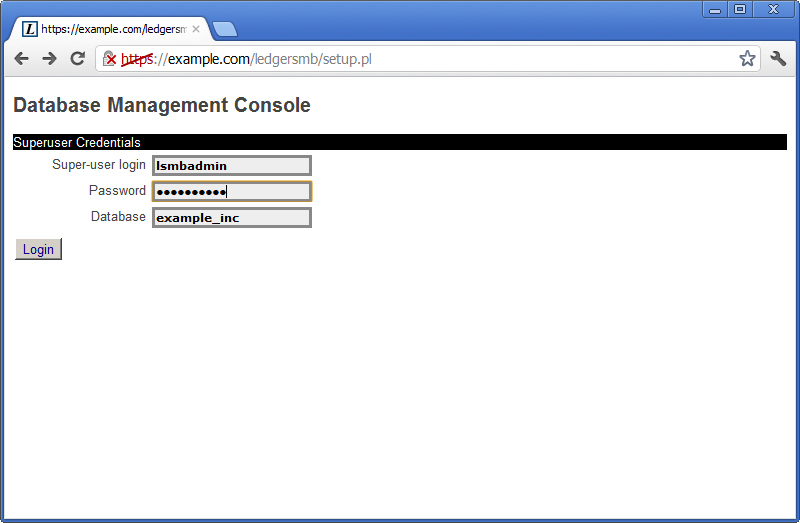
\includegraphics[width=0.8\textwidth]{dmc-create-step1.png}
\caption{setup.pl login screen}
\label{fig:setup-step1}
\end{figure}

\subsection{Step 2: Company creation}
\label{subsec-create-setup-create}

When creating a company database, there are a few things that are of importance:

\begin{itemize}
\item The name of the company database will be used at login time and hence
   will be used by all users - a choice of recognizable value is important
\item The value entered (and hence the company name) is case-sensitive
\item The name can't be more than 63 characters long
% \item ### others?
\end{itemize}

After choosing ``example\_inc'' as his company name, Jack clicks the Login button at which
time the screen from \figref{fig:setup-step2} shows up. The screen says the database doesn't yet exist and offers its creation.

\begin{figure}[h]
\centering
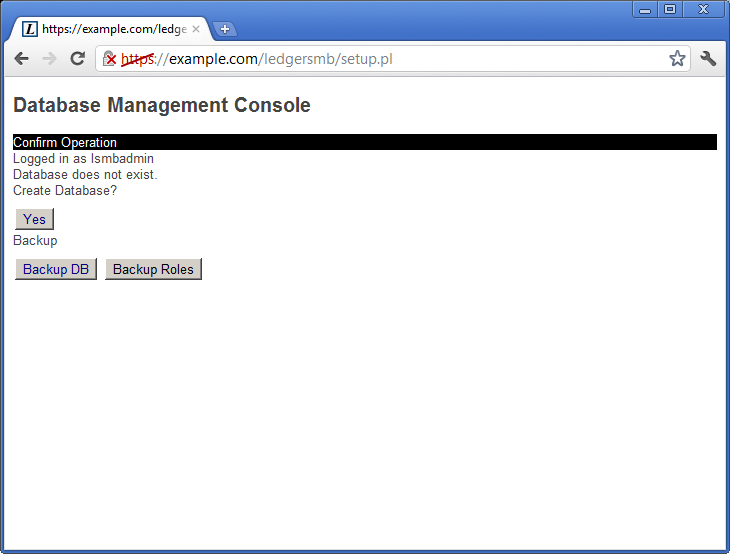
\includegraphics[width=7cm]{dmc-create-step2.png}
\caption{setup.pl company creation screen}
\label{fig:setup-step2}
\end{figure}

Jack clicks ``Yes'' to create the database and load it with LedgerSMB's database
schema, authorization rules and stored
procedures\footnote{Parts of the program inside the database.}. It may
take a while (30 seconds or more) for the next screen to appear\footnote{Note 
that during the creation of the database, logs are kept so that in case of
errors these can be reviewed either by the person running the installation or by
support personnel.  On Linux/Unix systems these are stored, by default, in
/tmp/ledgersmb/ and named dblog, dblog\_stderr and dblog\_stdout.}.

\subsection{Step 3: Selection of a Chart of Accounts}
\label{subsec-create-setup-select-coa}

LedgerSMB comes with numerous predefined charts of accounts\index{chart of accounts}. These have been grouped
per country making the selection of a chart a two-step procedure. setup.pl allows for
users wanting to define their own charts by offering a ``Skip'' button. This button
skips the process of loading a chart.

\begin{quote}
Note that you need to define a chart of accounts before you can meaningfully do anything
inside LedgerSMB. If you don't load a pre-defined one you'll need to create or upload
your own from inside the application once setup has completed.
\end{quote}

\figref{fig:setup-step3} shows the first screen in the \acrshort{CoA} selection procedure.
Here you select the country for which you want to use the \acrshort{CoA}. Note
that charts of accounts are highly country dependent and you may want to consult
an accountant if no default chart of accounts is included for your country.

As Jack runs his company in the United States, that's what he selects.

\begin{figure}[h]
\centering
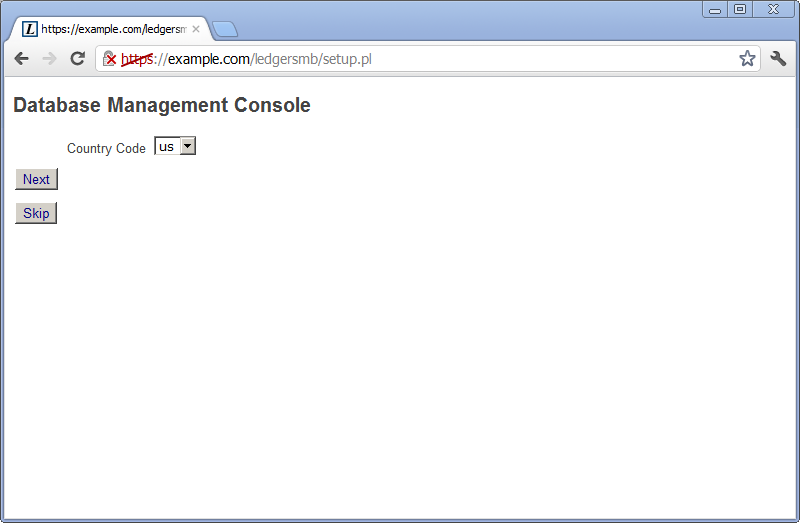
\includegraphics[width=7cm]{dmc-create-step3.png}
\caption{Chart of accounts - Country selection}
\label{fig:setup-step3}
\end{figure}

\figref{fig:setup-step4} shows the second screen in the chart of accounts selection procedure.
The drop down contains a list of all charts of accounts defined for the selected country.

Jack selects the \texttt{GeneralHierarchical.xml} chart of accounts: that will
leave him enough room to specialize the setup later if he has to, but for the time
being offers a broadly usable setup.

\begin{figure}[h]
\centering
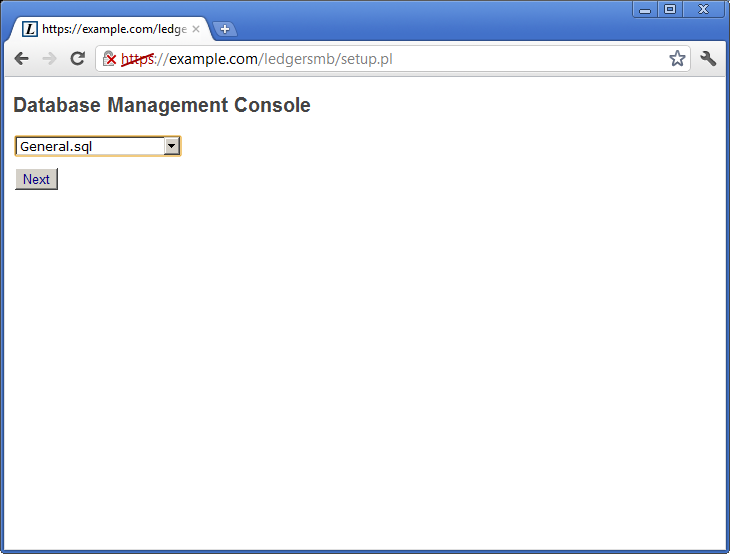
\includegraphics[width=7cm]{dmc-create-step4.png}
\caption{Chart of accounts - Chart selection}
\label{fig:setup-step4}
\end{figure}

\subsection{Step 4: Load template}
\label{subsec-create-setup-load-template}

LedgerSMB comes with a set of default reporting templates\index{templates}. 
These control the formatting of documents like invoices, checks, balance sheet, purchase orders, income statement, etc. 
Jack is now presented with the screen to load templates. LedgerSMB \ledgerSMBversion comes with a single choice\footnote{Administrators may define extra sets for users to be selected upon company creation; see \ref{sec-customization-company-creation-templates}}:
\begin{itemize}
        \item  \texttt{demo} -- Example template set for various output formats including PDF, HTML and Excel
\end{itemize}

\subsection{Step 5: Initial user}
\label{subsec-create-setup-initial-user}

In the previous step, the technical part of the company creation procedure
was completed. However, it's not possible to log in to the company yet. 
\figref{fig:setup-step5} shows the next step in the setup process:
 the user creation screen. The fields shown have
the same meaning as those discussed as part of user management in \secref{sec-user-creation}.

\begin{figure}[h]
\centering
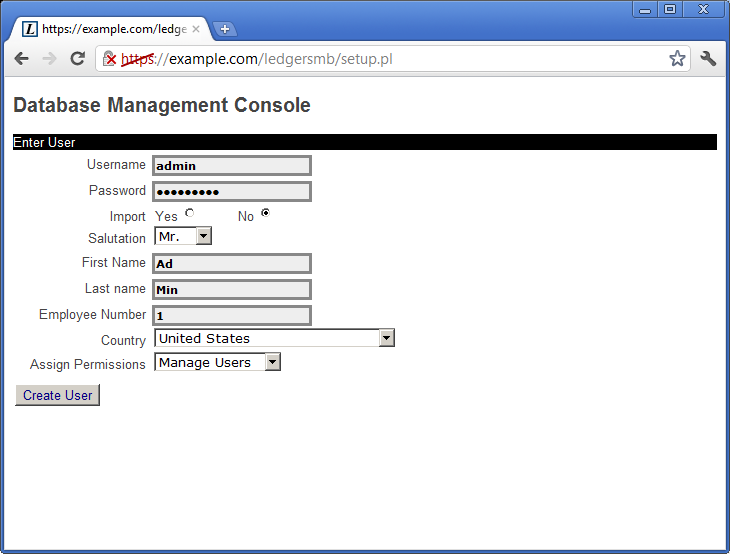
\includegraphics[width=7cm]{dmc-create-step5.png}
\caption{setup.pl initial user creation screen}
\label{fig:setup-step5}
\end{figure}

Jack chooses to create an administrative user called \texttt{admin} who will be authorized
to do everything in the application. Later on he will also create a user \texttt{jack}
who will be authorized to do everything but changing the configuration and doing application administration.
He'll use the latter user to log in for day to day operations. This will help him prevent changing settings by accident.

Note that none of the fields in this screen are optional. If the name of the user being created
isn't already used with other companies, leave the \texttt{Import} option set to \texttt{No},
otherwise please read the chapter on user creation mentioned above.

\begin{quotation}
Note: The password you enter here is a temporary one which will remain in effect
\textbf{for 24 hours only}. Be sure to execute the steps in \secref{sec-first-login-ramp-up} before
these 24 hours elapse, because the user will be disabled after that.
\end{quotation}

Jack proceeds to enter the values as follows:
\begin{longtable}{ llp{6cm} }
        Field & Value & Description \\ \hline
        \endhead
        User Name & \texttt{admin} & The login user name\\
        Password & \texttt{asdfg} & The password to use for your first login\\
        Create New User & \texttt{Checked} & \\
        Import Existing User & \texttt{Unchecked} & Only used when the user exists in another database\\
        Salutation & \texttt{Mr.} & \\
        First Name &  \texttt{Ad} & Used in combination with Last Name to identify the user \\
        Last Name & \texttt{Min} & \\
        Employee Number & \texttt{1} & \\
        Date of Birth & \texttt{1/1/2000} & not used by the application \\
        Tax ID/SSN & \texttt{0} & Tax or \acrshort{SSN}; not used by the application \\
        Country & \texttt{United States} & \\
        Assign Permissions & \texttt{Full Permissions} & \\
        \\
        \caption{Create first user entry data}
        \label{tbl:setupp-step5-user-entry-data}
\end{longtable}

@@@TODO: Replace figure below: it looks different these days (missing statistics section)
\begin{figure}[h]
\centering
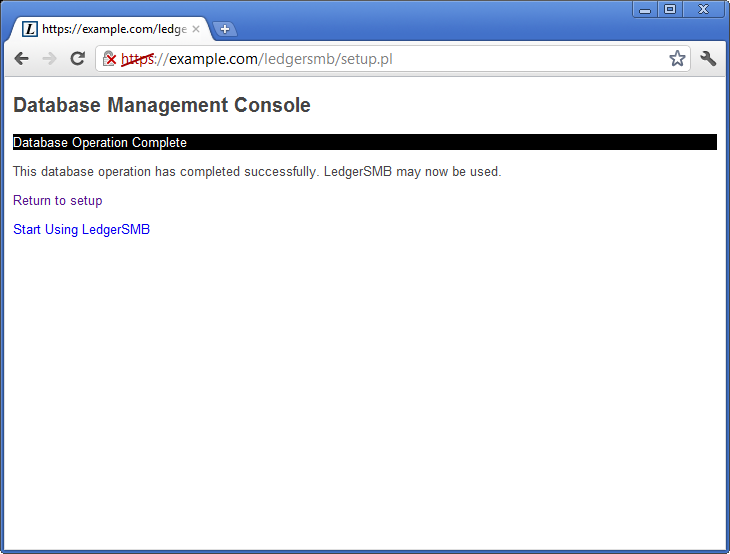
\includegraphics[width=7cm]{dmc-create-step6.png}
\caption{setup.pl successful completion screen}
\label{fig:setup-step6}
\end{figure}

Jack has created his company database and now sees the
 ``Database Management Console"  screen as shown in \figref{fig:setup-step6}.

By selection \texttt{Start using LedgerSMB} in the ``Database Operation Complete" section of the screen his story continues in
the next chapter ``The first login''.

\chapter{The first login}
\label{cha-first-login}

\section{Introduction}
\label{sec-first-login-introduction}

After the company database has been created by executing the procedure described in the last
chapter it is still an empty shell which needs to be populated. The correct data
needs to be entered for things like bank accounts and company contact data to be used
on invoices.

These steps have to be completed before LedgerSMB can be used meaningfully: these
settings have to be present for many workflows. A major reason is that with LedgerSMB
- as most \gls{erp} - financial
consequences of events in many workflows are directly reflected in the company's books.
Some accounting related settings have to be completed before LedgerSMB can do so.

This chapter documents the steps to create a basic usable configuration for Example Inc. 
It assumes that
one of the default chart of accounts was selected as shown in \charef{cha-company-creation} or 
that a custom chart of accounts was imported using the instructions in \secref{subsubsec-coa-importing}. 
Whatever method was chosen, this chapter assumes that a chart of accounts is available.

\section{Steps to the first login}
\label{sec-first-login-ramp-up}

Jack is ready for his first login and should see the screen as shown in \figref{fig:login-screen}.

If this screen is not shown then Jack navigates to 
\url{https://example.com/ledgersmb/login.pl} to access the login screen.

\subsection{Login screen}
\label{subsec-first-login-screen}

\begin{figure}[h]
\centering
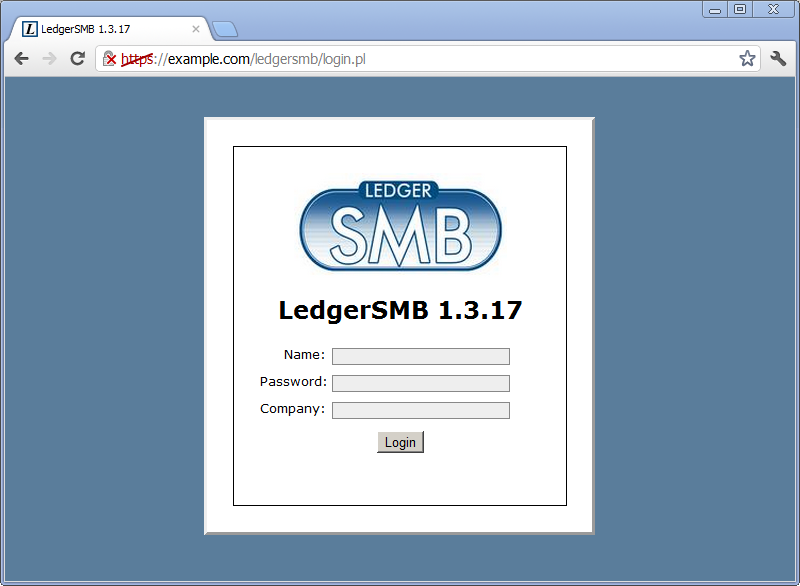
\includegraphics[width=7cm]{dmc-create-final.png}
\caption{login.pl opening screen}
\label{fig:login-screen}
\end{figure}

The login screen shows three fields which Jack proceeds to fill in as follows:

\begin{longtable}{ llp{6cm} }
        Field & Value & Description \\ \hline
        \endhead
        Name & \texttt{admin} & The login user name\\
        Password & \texttt{asdfg} & The password to use for your first login\\
        Company & \texttt{example\_inc} & The name of the company database \\
\end{longtable}

% \begin{description}
% \item[Name] The user name created during database setup; Jack uses \texttt{admin}
% \item[Password] The password - in this case for Jack's \texttt{admin} user
% \item[Company] The name of the database created; Jack uses \texttt{example\_inc}
% \end{description}

After entering all of the information and tapping the \texttt{Login} button Jack will see an alert letting
him know that his password will expire today.  Jack clicks \texttt{OK} to dismiss the alert.

\subsection{Selecting a password}
\label{subsec-first-login-password}

After successful login, the system shows the Welcome to LedgerSMB  screen as depicted in
\figref{fig:login-welcome-screen}.

\begin{figure}[h]
        \centering
        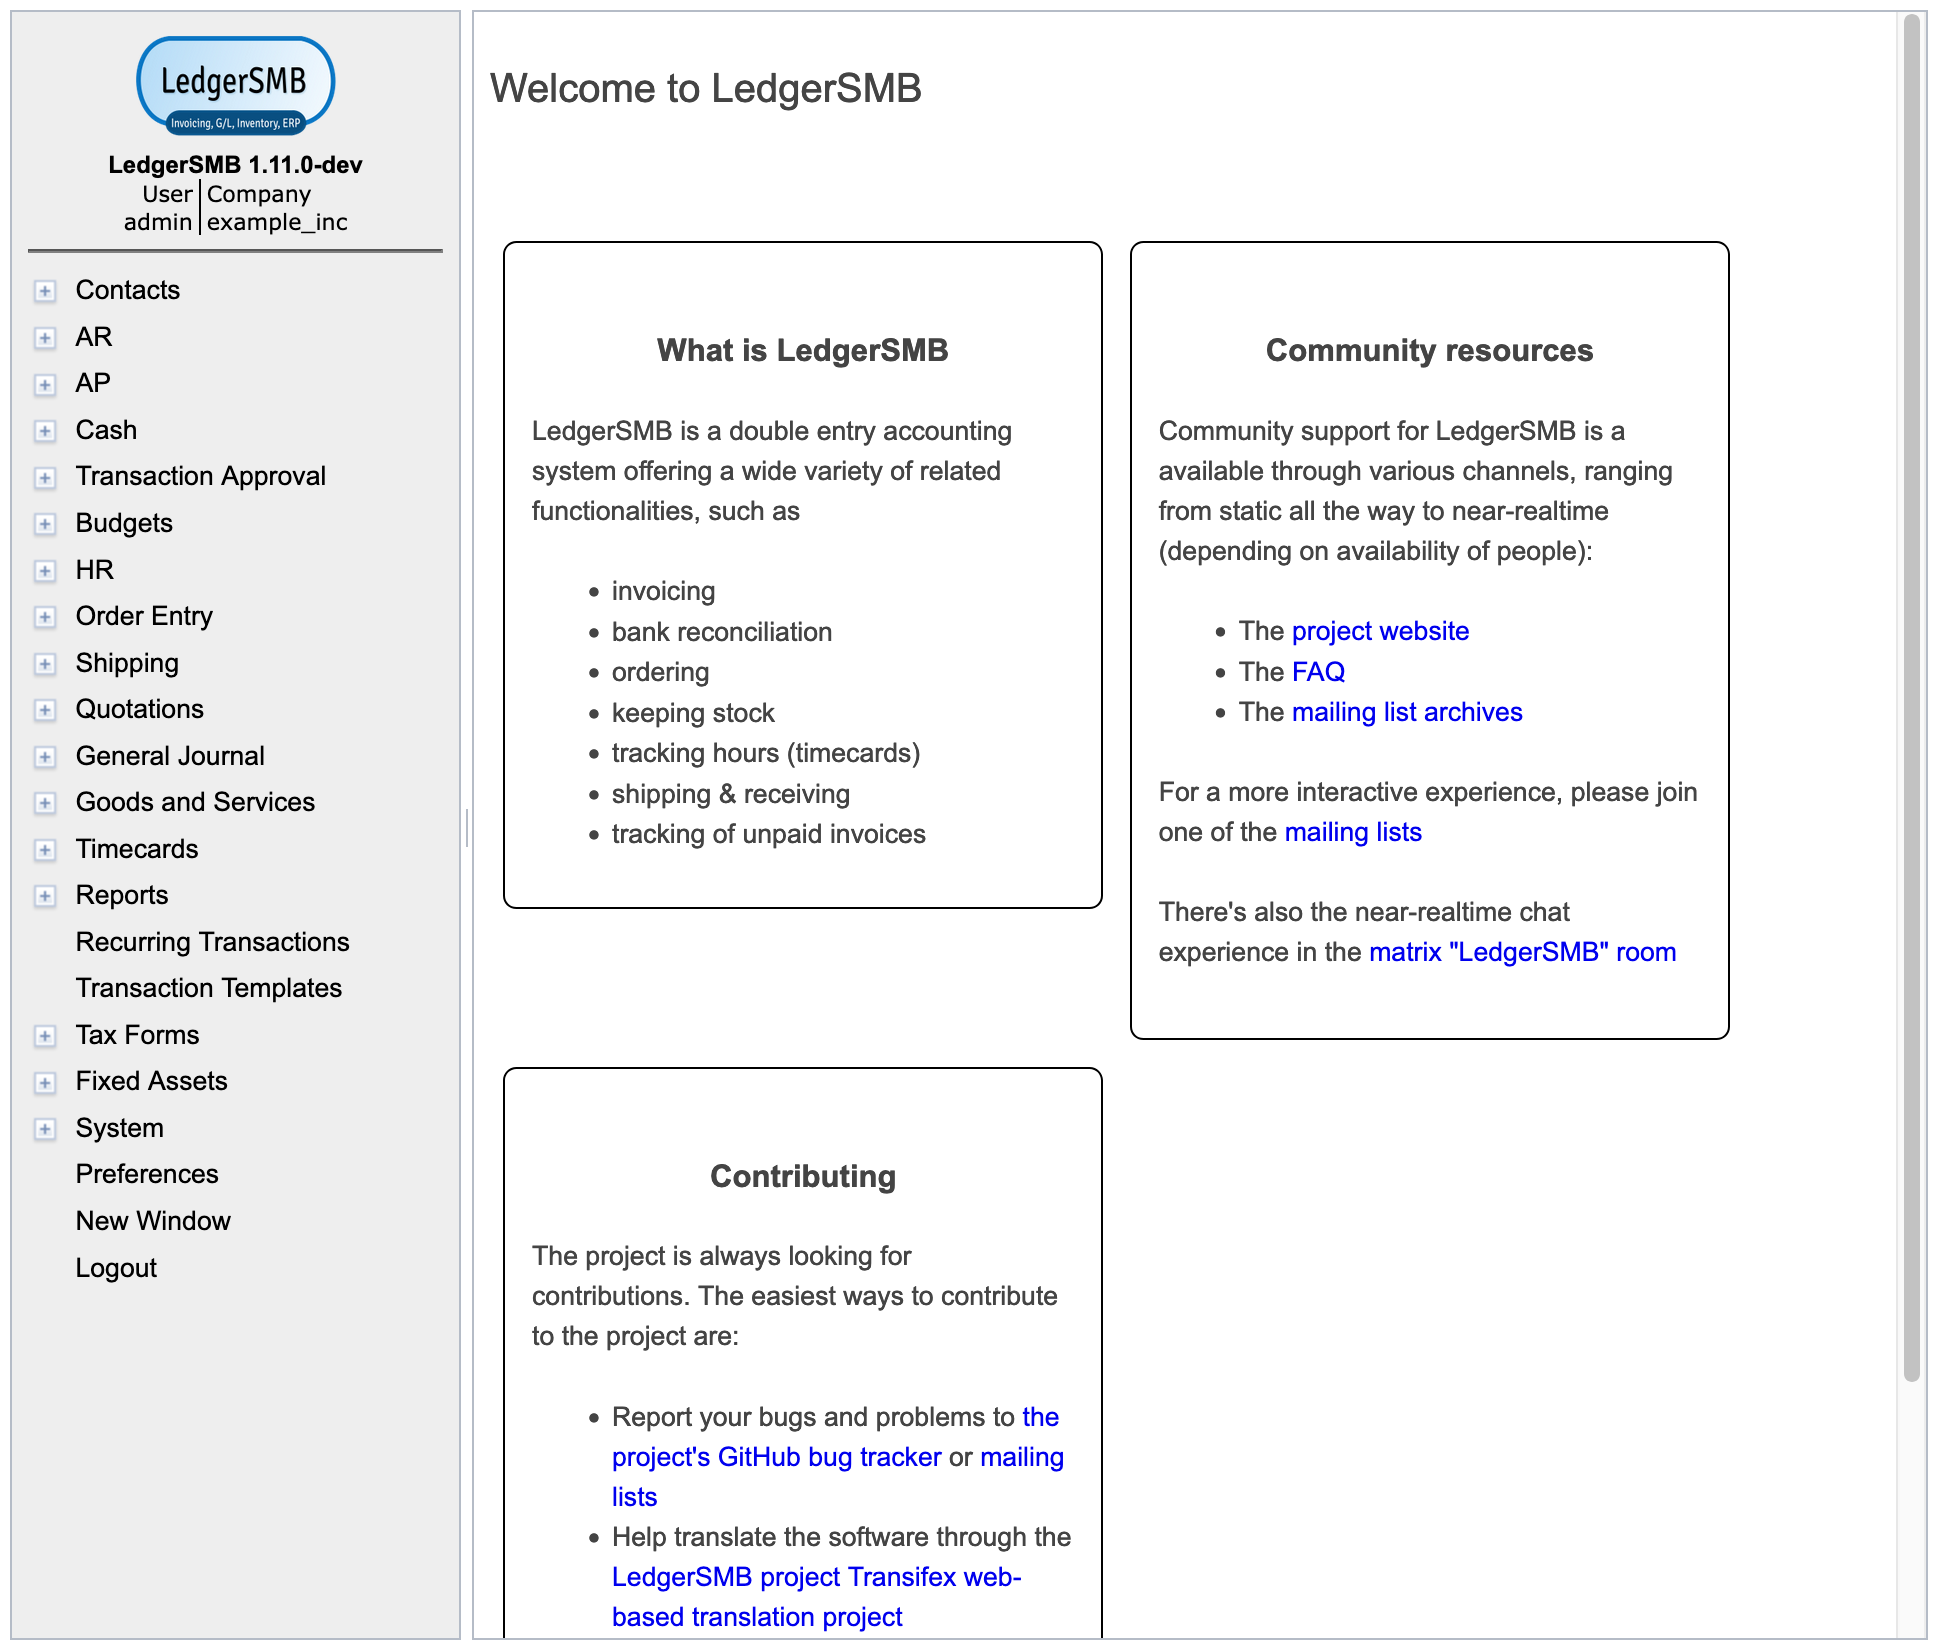
\includegraphics[width=7cm]{welcome.png}
        \caption{login.pl welcome screen}
        \label{fig:login-welcome-screen}
\end{figure}

The
initial password has a 24-hour validity limit to prevent unused user accounts from posing
a security risk.  

To set a new password Jack navigates to \menupath{Preferences \ma Password} and sees the 
screen as depicted in \figref{fig:first-user-password}.

The new password that Jack chooses will be different than any password used before and 
different than the temporary password set by the administrator.
Not clicking the \texttt{Save} button means the password remains unchanged and the
24-hour limit remains in effect.

\begin{figure}[H]
\centering
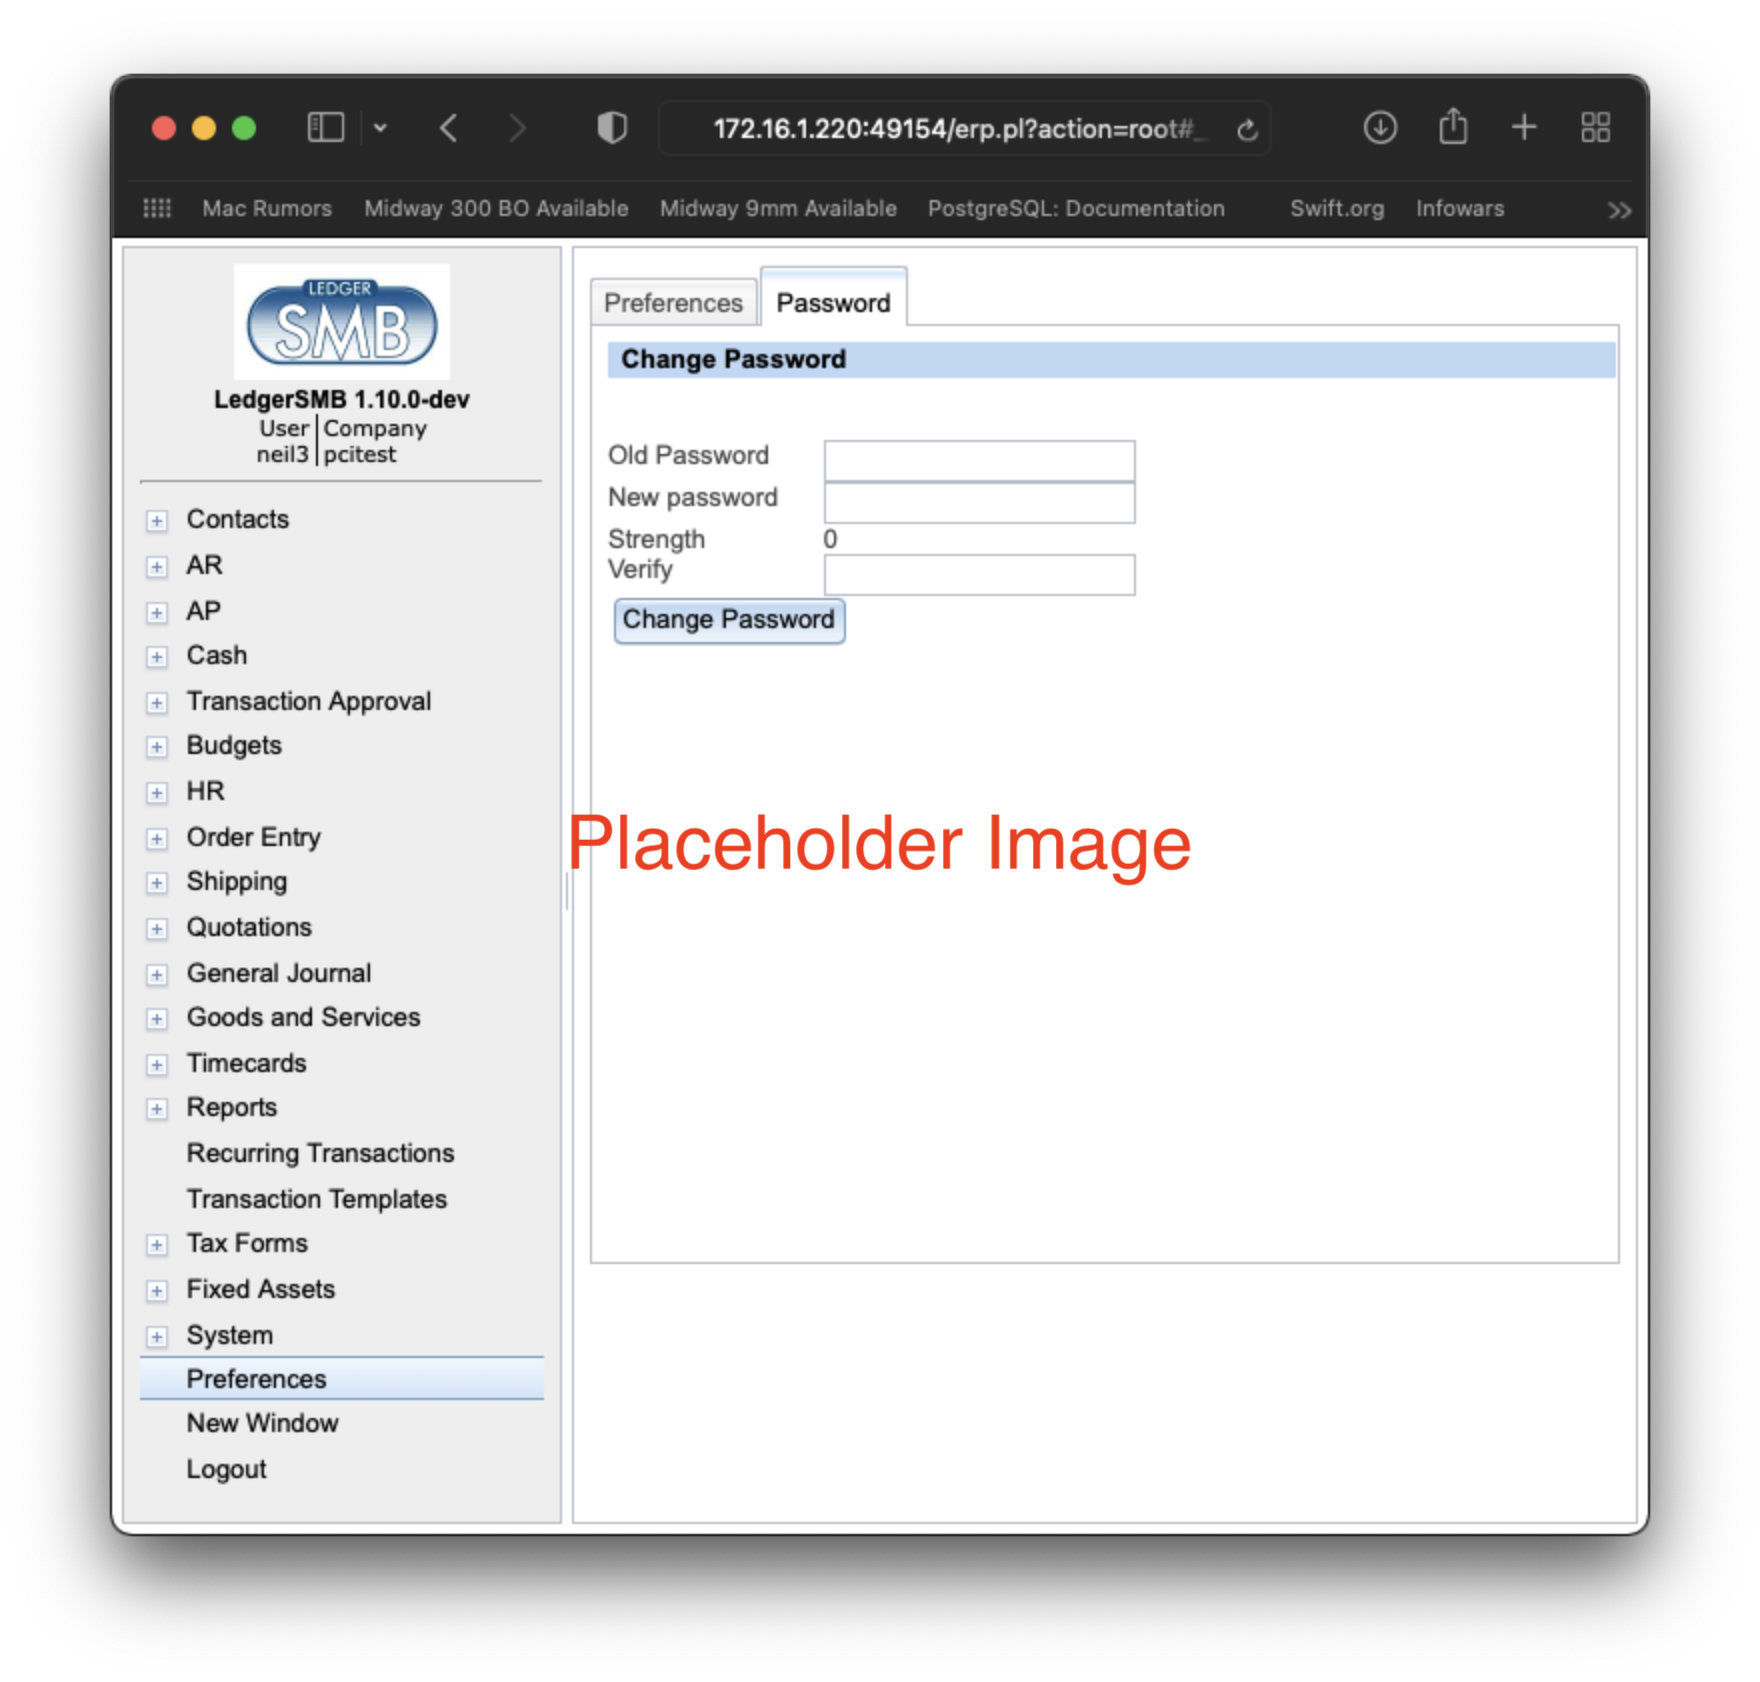
\includegraphics[width=7cm]{user-password.png}
\caption{Password change screen}
\label{fig:first-user-password}
\end{figure}

Jack enters the information in the Change Password screen as follows:
\begin{longtable}{ llp{6cm} }
        Field & Value & Description \\ \hline
        \endhead
        Old Password & \texttt{asdfg} & The old password set by the administrator using setup.pl\\
        New Password & \texttt{lkjhg} & The new password that Jack wants to use for admin\\
        Verify & \texttt{lkjhg} &  Repeats the new password that Jack wants to use for admin\\
        \\
        \caption{First Login - Change initial password data}
        \label{fig:first-user-change-initial-password}
\end{longtable}

%\begin{description}
%       \item[Old Password] The old password originally set by the administrator using \texttt{setup.pl}
%       \item[New Password] The new password for Jack's account.
%       \item[Verify] The new password for Jack's account.
%\end{description}

Jack then clicks the \texttt{Change Password} button.

The new password has a validity of determined by the \texttt{Password Duration} setting
from the \menupath{System \ma Defaults} screen. User management is discussed is detail in \charef{cha-user-management}.

Login will be denied to users with expired passwords; they can request
password resets through user admins.

\subsection{Setting user preferences}
\label{subsec-setting-user-preferences}

Jack clicks on the tab \texttt{Preferences} and the system shows the Preferences screen 
as depicted in \figref{fig:user-preferences}

\begin{figure}[H]
        \centering
        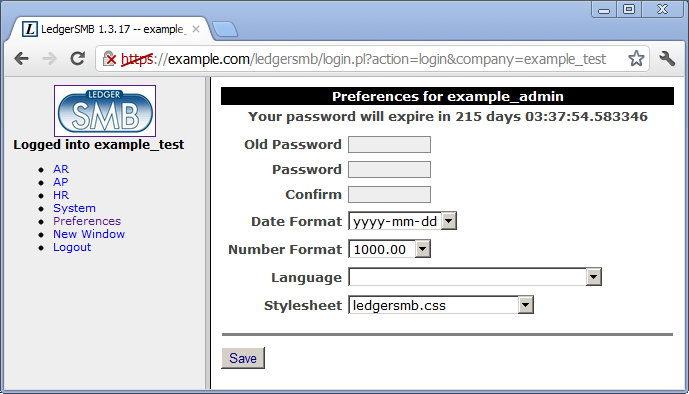
\includegraphics[width=7cm]{user-preferences.png}
        \caption{User preferences}
        \label{fig:first-user-preferences}
\end{figure}

Jack selects his language, in this case \texttt{American English} and clicks \texttt{Save}.

\subsection{Setting system defaults}
\label{subsec-setting-system-defaults}

Out of the box, LedgerSMB contains reasonable system defaults, but Jack needs to add some specific company information.
In order to do so, Jack navigates to \menupath{System \ma Defaults} and sees the screen depicted in \figref{fig:first-user-system-defaults}.
 
\begin{figure}[H]
        \centering
        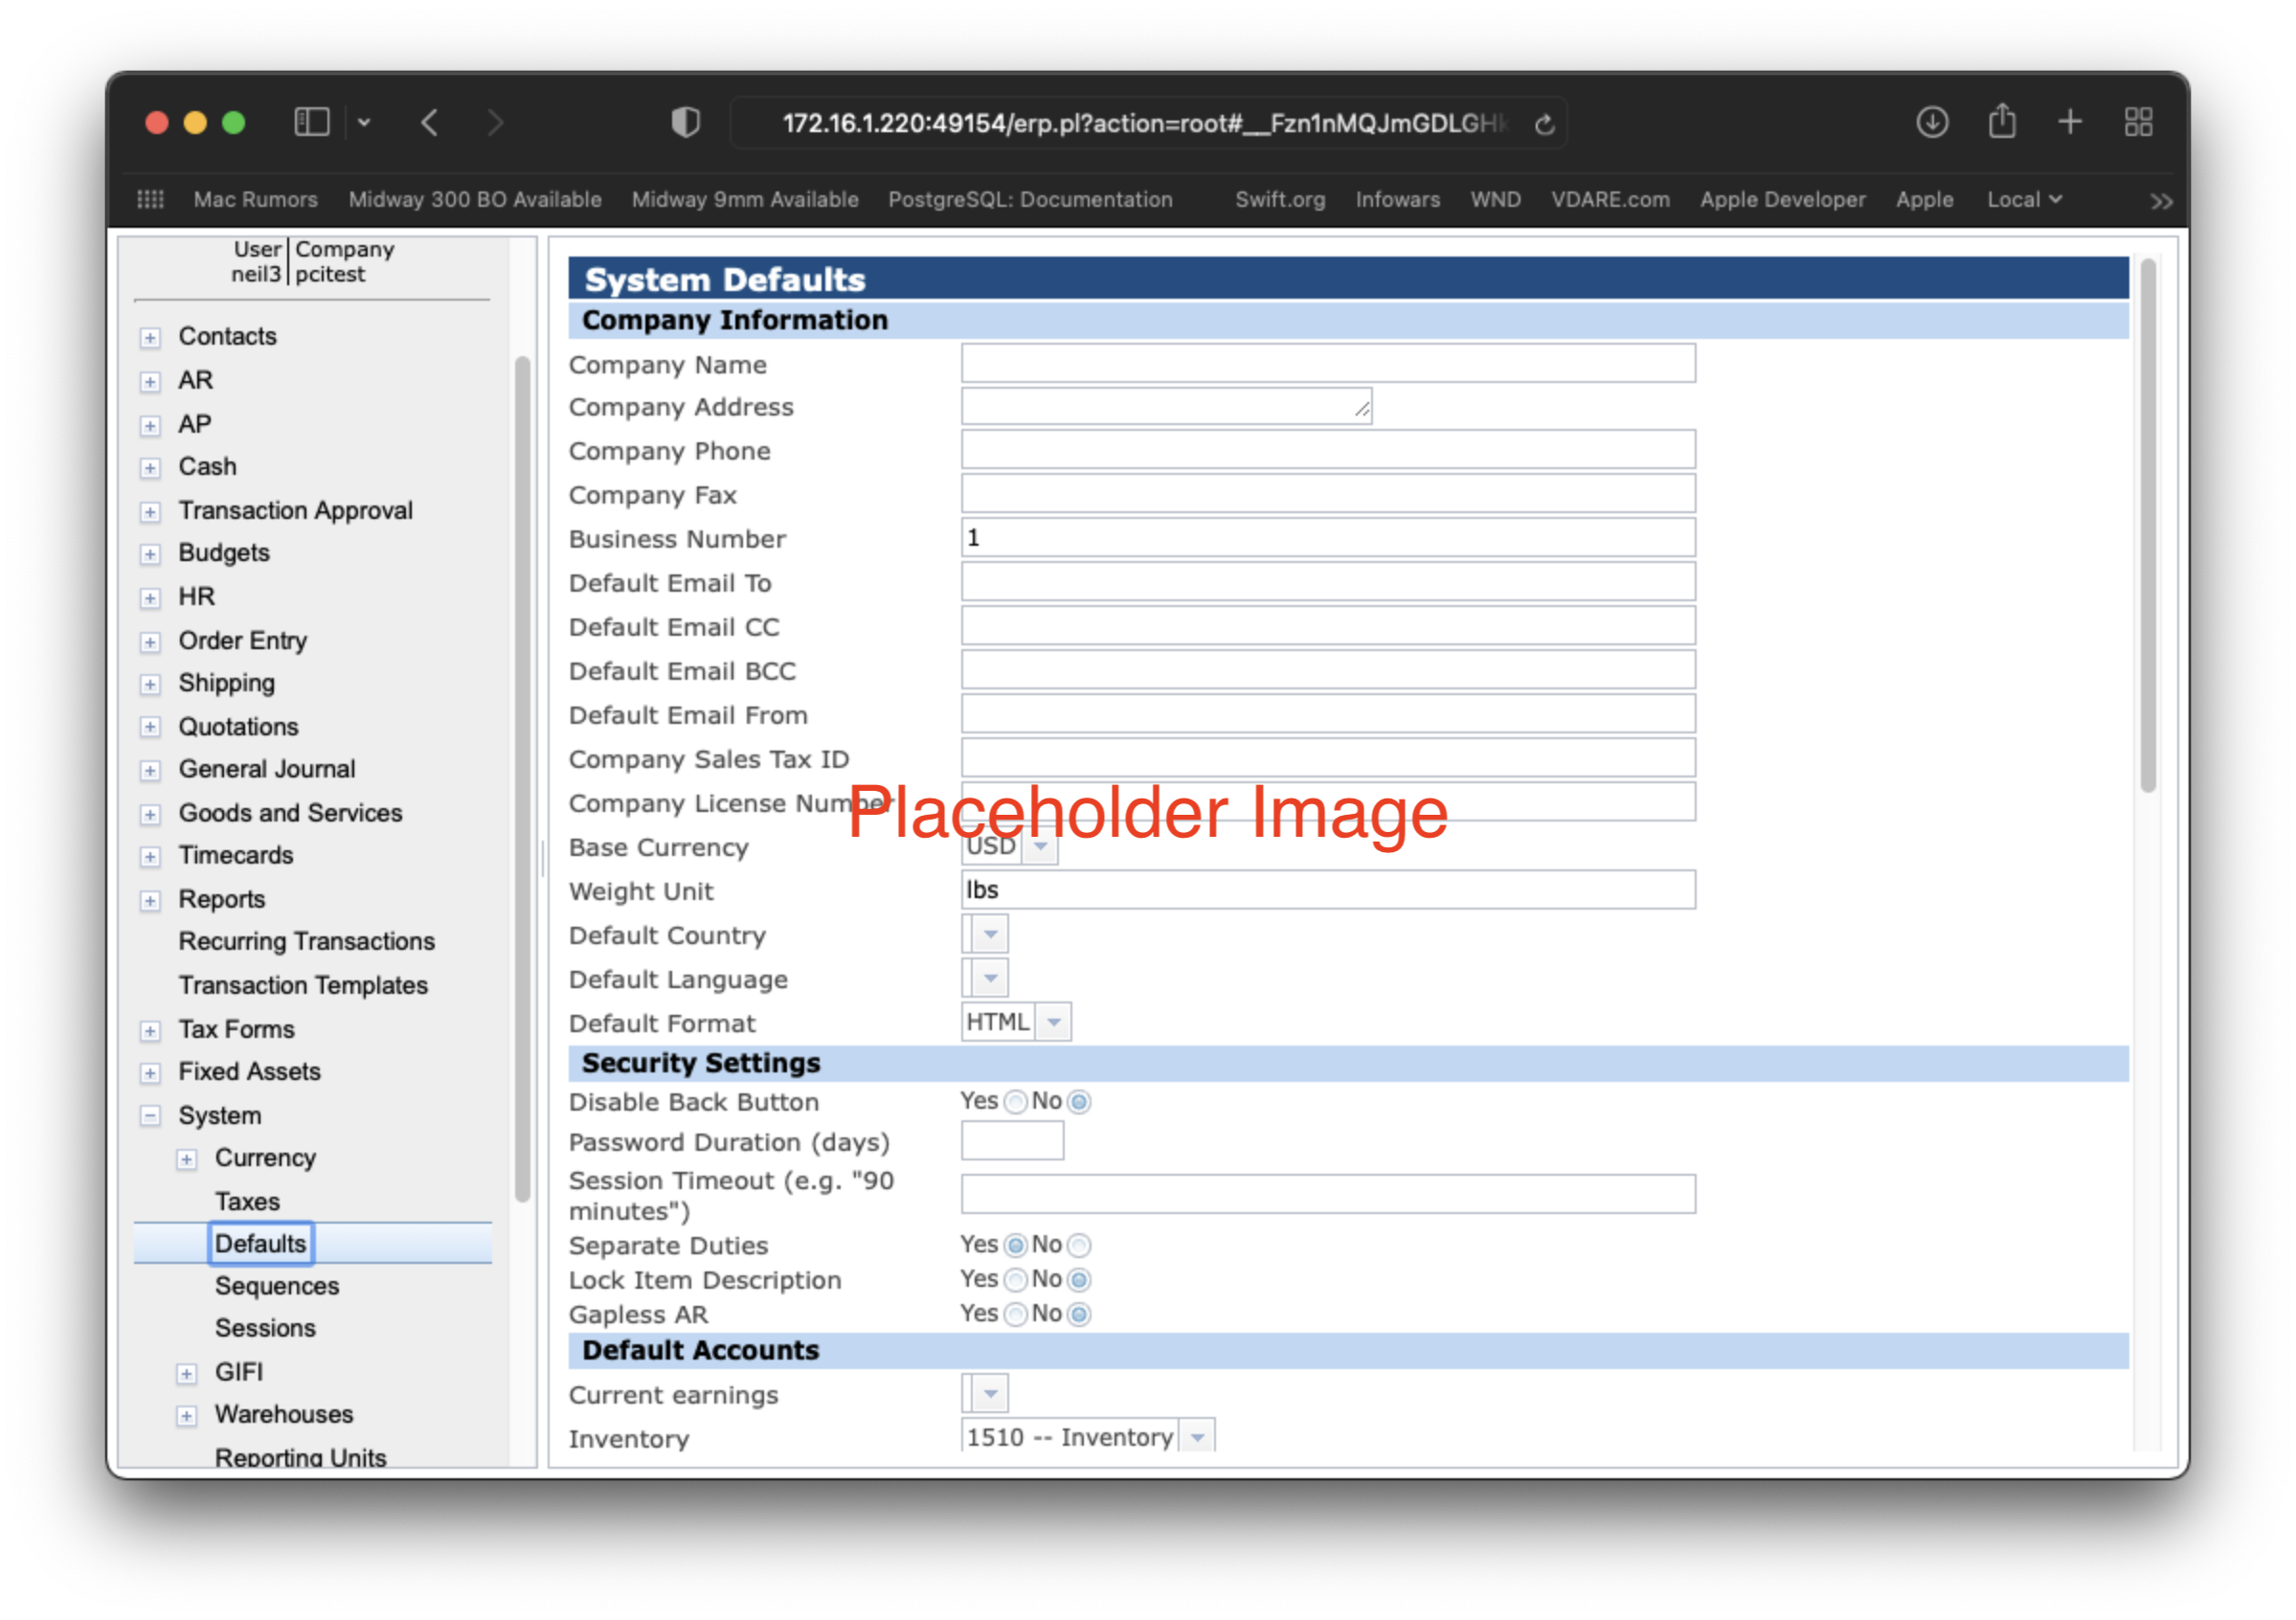
\includegraphics[width=7cm]{system-defaults.png}
        \caption{System defaults}
        \label{fig:first-user-system-defaults}
\end{figure}

Jack sets the following defaults:
\begin{longtable}{ llp{6cm} }
        Field & Value & Description \\ \hline
        \endhead
        Company Name & \texttt{Example Inc.} & \\
        Company Address &  \makecell[l]{\texttt{215 Example St} \\  \texttt{Any City, CA}} & Note the use of the new line\\
        Company Phone &  \texttt{555 836 2255} & \\
        Business Number &  \texttt{12345} & e.g. Chamber of commerce number\\
        Default Email From & \texttt{info@example.com} & \\
        Default Country & \texttt{United States}  & \\
        Default Language &  \texttt{English (US)} & \\
        Password Duration &  \texttt{180} & Days\\
        \\
\caption{First Login - Change user defaults data}
\label{fig:first-user-user-default-data}
\end{longtable}

%\begin{itemize}
%       \item \textbf{Company Name} to \texttt{Example Inc.}
%       \item \textbf{Company Address} to  \texttt{215 Example street, Any City, CA}
%       \item \textbf{Company Phone} to \texttt{555 836 2255}
%       \item \textbf{Business Number} (e.g. Chamber of commerce number) to \texttt{12345}
%       \item \textbf{Default Email From} to \texttt{info@example.com}
%       \item \textbf{Default Country} to \texttt{United States} 
%       \item \textbf{Default Language} to \texttt{English (US)}
%       \item \textbf{Password Duration} to \texttt{180}
%\end{itemize}

A more elaborate description of the parameters in this screen is provided in subsection
\ref{subsec-company-config-defaults}.

\section{Setting up a bank account or credit card}
\label{sec-first-login-setup-bank-account}

As part of the start up activities of his company, Jack comes to an agreement with the
bank for three products:

\begin{itemize}
\item A current account with number ``C54769''
\item Deposit account with number ``D54990''
\item Credit card with a number ending with ``.7734''
\end{itemize}

Most accounting systems - LedgerSMB included - use separate GL accounts to represent
each bank account. This allows easy reconciliation of the ending balance on the bank
account with the balance in the books.

Knowing this, Jack looks up the example bank account from his preconfigured US chart of
accounts using the \menupath{General Journal \ma Chart of Accounts} menu as
shown in \figref{fig:bank-setup1}.

\begin{figure}[h]
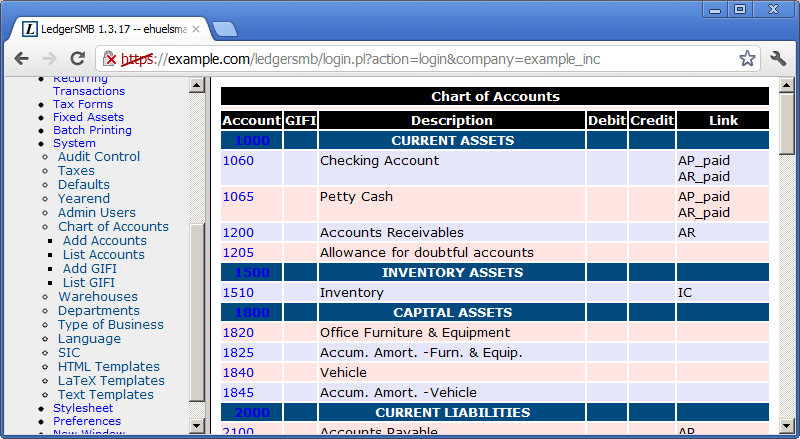
\includegraphics[width=\linewidth]{setup-bank-account1.png}
\caption{Bank account setup - menu items}
\label{fig:bank-setup1}
\end{figure}

Jack adds the new bank accounts by doing the following:

\begin{enumerate}
\item Click on ``1060''
\item The screen appears as shown in \figref{fig:bank-setup2} appears 
\item Change the Description ``Checking Account'' to ``Checking Account C54769''
\item Click ``Save''
\item In the same screen change the Account Number to ``1061''
\item Change the Description to ``Cash Deposit Account D54990''
\item Click ``Save as new''
\item In the same screen change the Account Number to ``1062""
\item Change the description to ``Credit Card xxxx.xxxx.7734''
\item Click ``Save as new''
\end{enumerate}

\secref{sec-coa-account-options} discusses the options in detail - for now using the
settings as configured for the sample checking account will do.

\begin{figure}[h]
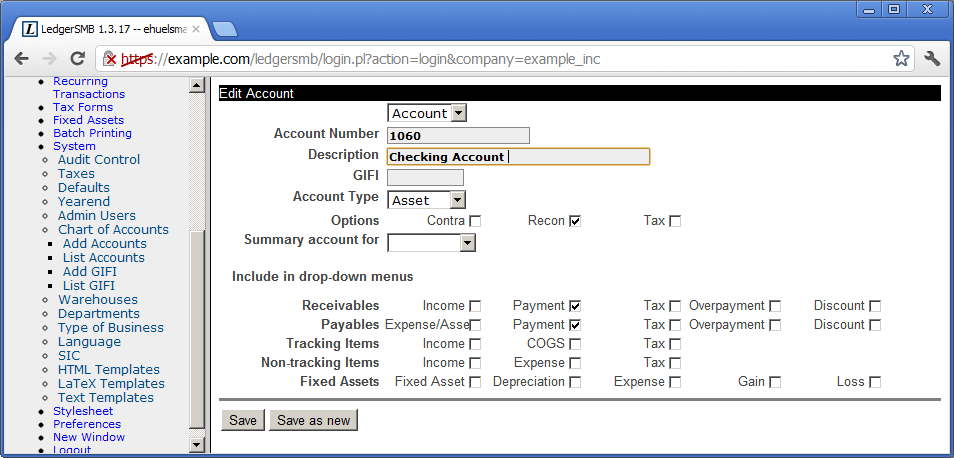
\includegraphics[width=\linewidth]{setup-bank-account2.png}
\caption{Bank account setup - account setup screen}
\label{fig:bank-setup2}
\end{figure}


\section{Checking and adjusting the chart of accounts}
\label{sec-first-login-coa-check}

First and foremost the chart of accounts serves to register income, expenses,
assets and liabilities in categories which support financial decision making or
regulatory requirements. When checking his chart of accounts, this is the first
thing Jack checks for.

Many business events in LedgerSMB trigger the creation of financial transactions.
If the configuration required for these transactions to be created isn't in place,
users won't be able to complete their workflows. 

\subsection{Accounts list}
\label{subsec-first-login-accounts-list}

Jack wants to make sure his chart of accounts fits his purposes. To perform these
checks Jack goes into the \menupath{General Journal \ma Chart of Accounts} page. For now, he finds
the ledger to be in order. Although the single Sales account stands out a bit against
the numerous expense accounts, it turns out that there is also a single Purchases
account on which all the expenses for parts purchases are going to be booked.

He decides that if this isn't enough, he can add accounts later.
\footnote{Note that Jack will discover in \secref{sec-stock-defining-vendors} that
he does indeed need to create additional accounts to support sales and
purchase discounts.}


\section{Checking sales tax rates}
\label{sec-first-login-checking-tax-rates}

First off, Jack asserts that a sales tax\footnote{Sales tax may be called \gls{VAT}
in some jurisdictions.} account has been provisioned. He finds it
in the Current Liabilities section of his \gls{CoA}. In his jurisdiction there
is only one sales tax rate applicable at any one time, which means this single account
will suit his needs just fine. If he had been in a jurisdiction with multiple tax rates
applicable, e.g. different rates for different types of goods, he would have been
required to create more accounts.

The procedure to create more sales tax accounts is the same as the one used in
\secref{sec-first-login-setup-bank-account}, with the notable difference that this time the base account
to be used is the sales tax account.

With the accounts in place, the tax rates have to be checked and possibly adjusted.
To do so, Jack navigates to the \menupath{System \ma Taxes} page as shown in \figref{fig:setup-tax-rates}.

\begin{figure}[h]
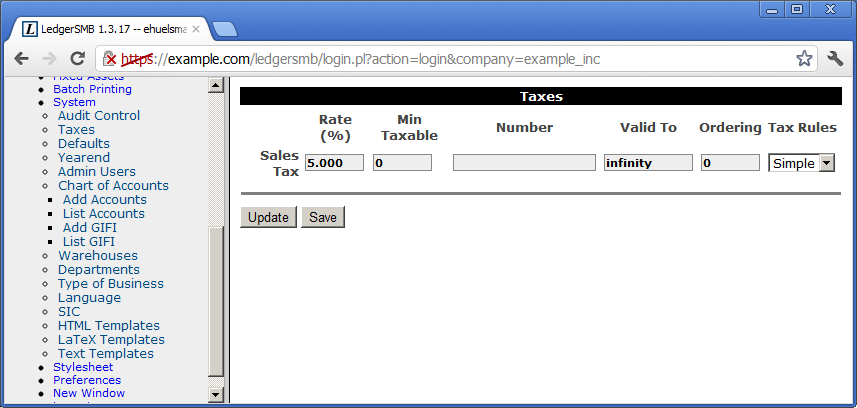
\includegraphics[width=\linewidth]{setup-tax-rates.png}
\caption{Tax rate adjustment screen}
\label{fig:setup-tax-rates}
\end{figure}

The rate shown (5\%) is exactly what Jack needs. The procedure to set rates is a bit
long to describe and hence has its own chapter. Please refer to \charef{cha-taxes} for
details on how to change taxes.

\chapter{Building up stock}
\label{cha-building-up-stock}

\section{Overview}
\label{sec-stock-overview}

In this chapter Jack goes through the process of setting up LedgerSMB for his
trade activities in computer parts, which includes deciding which parts he wants to
resell. From there on he goes to contact a vendor to request a quotation, convert that
to an order and receive goods into inventory and invoices into accounts payable.

To prepare LedgerSMB for his parts sales and purchases, Jack needs to configure Parts.
The system records inventory for parts and assemblies. Jack won't use them for his
business. There's more on assemblies in \secref{subsec-assemblies-definition}.

Once set up, Jack is ready to execute the ordering process. Even though the process
is described here from a purchasing perspective, sales work the same way with the roles
reversed (Jack will act as a vendor in the sales process).

To start his purchase, Jack creates a \gls{rfq} document which
he sends one or multiple vendors to let them know he's interested in their products.

The vendor responds to Jack's request by issuing a Quotation. From a legal perspective
a quotation is a document which promises to deliver the requested goods or services at a
certain rate - subject to conditions specifically mentioned. If Jack accepts the quotation
and meets the conditions, the vendor is obligated to deliver.

In response to the quotation, Jack will place an order with the vendor to indicate
acceptance of the quotation (or he can let the
it expire). When he places the order, that legally means he agrees to the terms
and conditions in the quotation. If the vendor delivers the goods or services as per the
order, Jack has accepted the legal obligation to pay.

The vendor responds to the order by shipping the goods and services as well
as sending an invoice. The invoice legally means the vendor considers to have a claim on the assets
of Jack's company. Jack creates a vendor invoice in his system to record the claim on his
company by the vendor and the vendor creates a sales invoice in their system to do the same.

As a result of the above it's considered bad practice to delete or change invoices once
created. The accepted process to adjust invoices is to generate a debit invoice (for purchases)
or a credit invoice (for sales) to ``undo'' the effects of the invoice and letting the other party
know about it. Then a new invoice can be generated with the appropriate content. However,
when the order process is correctly followed from order to invoice chances of sending the wrong
invoice are greatly reduced.

\section{Defining parts}
\label{sec-stock-parts}

Jack needs to enter a large number of items he'll be offering in his new shop. He starts out
with the easy ones: the ones which will be sold as single items.

\subsection{Single items}
\label{subsec-stock-parts-single-item}

Jack chooses a 5TB hard drive by Samsung to be entered into the system as the first item.
To do so, he goes to the \menupath{ Goods and Services \ma Add part} page from the menu
as shown in \figref{fig:setup-add-part}.

\begin{figure}[h]
        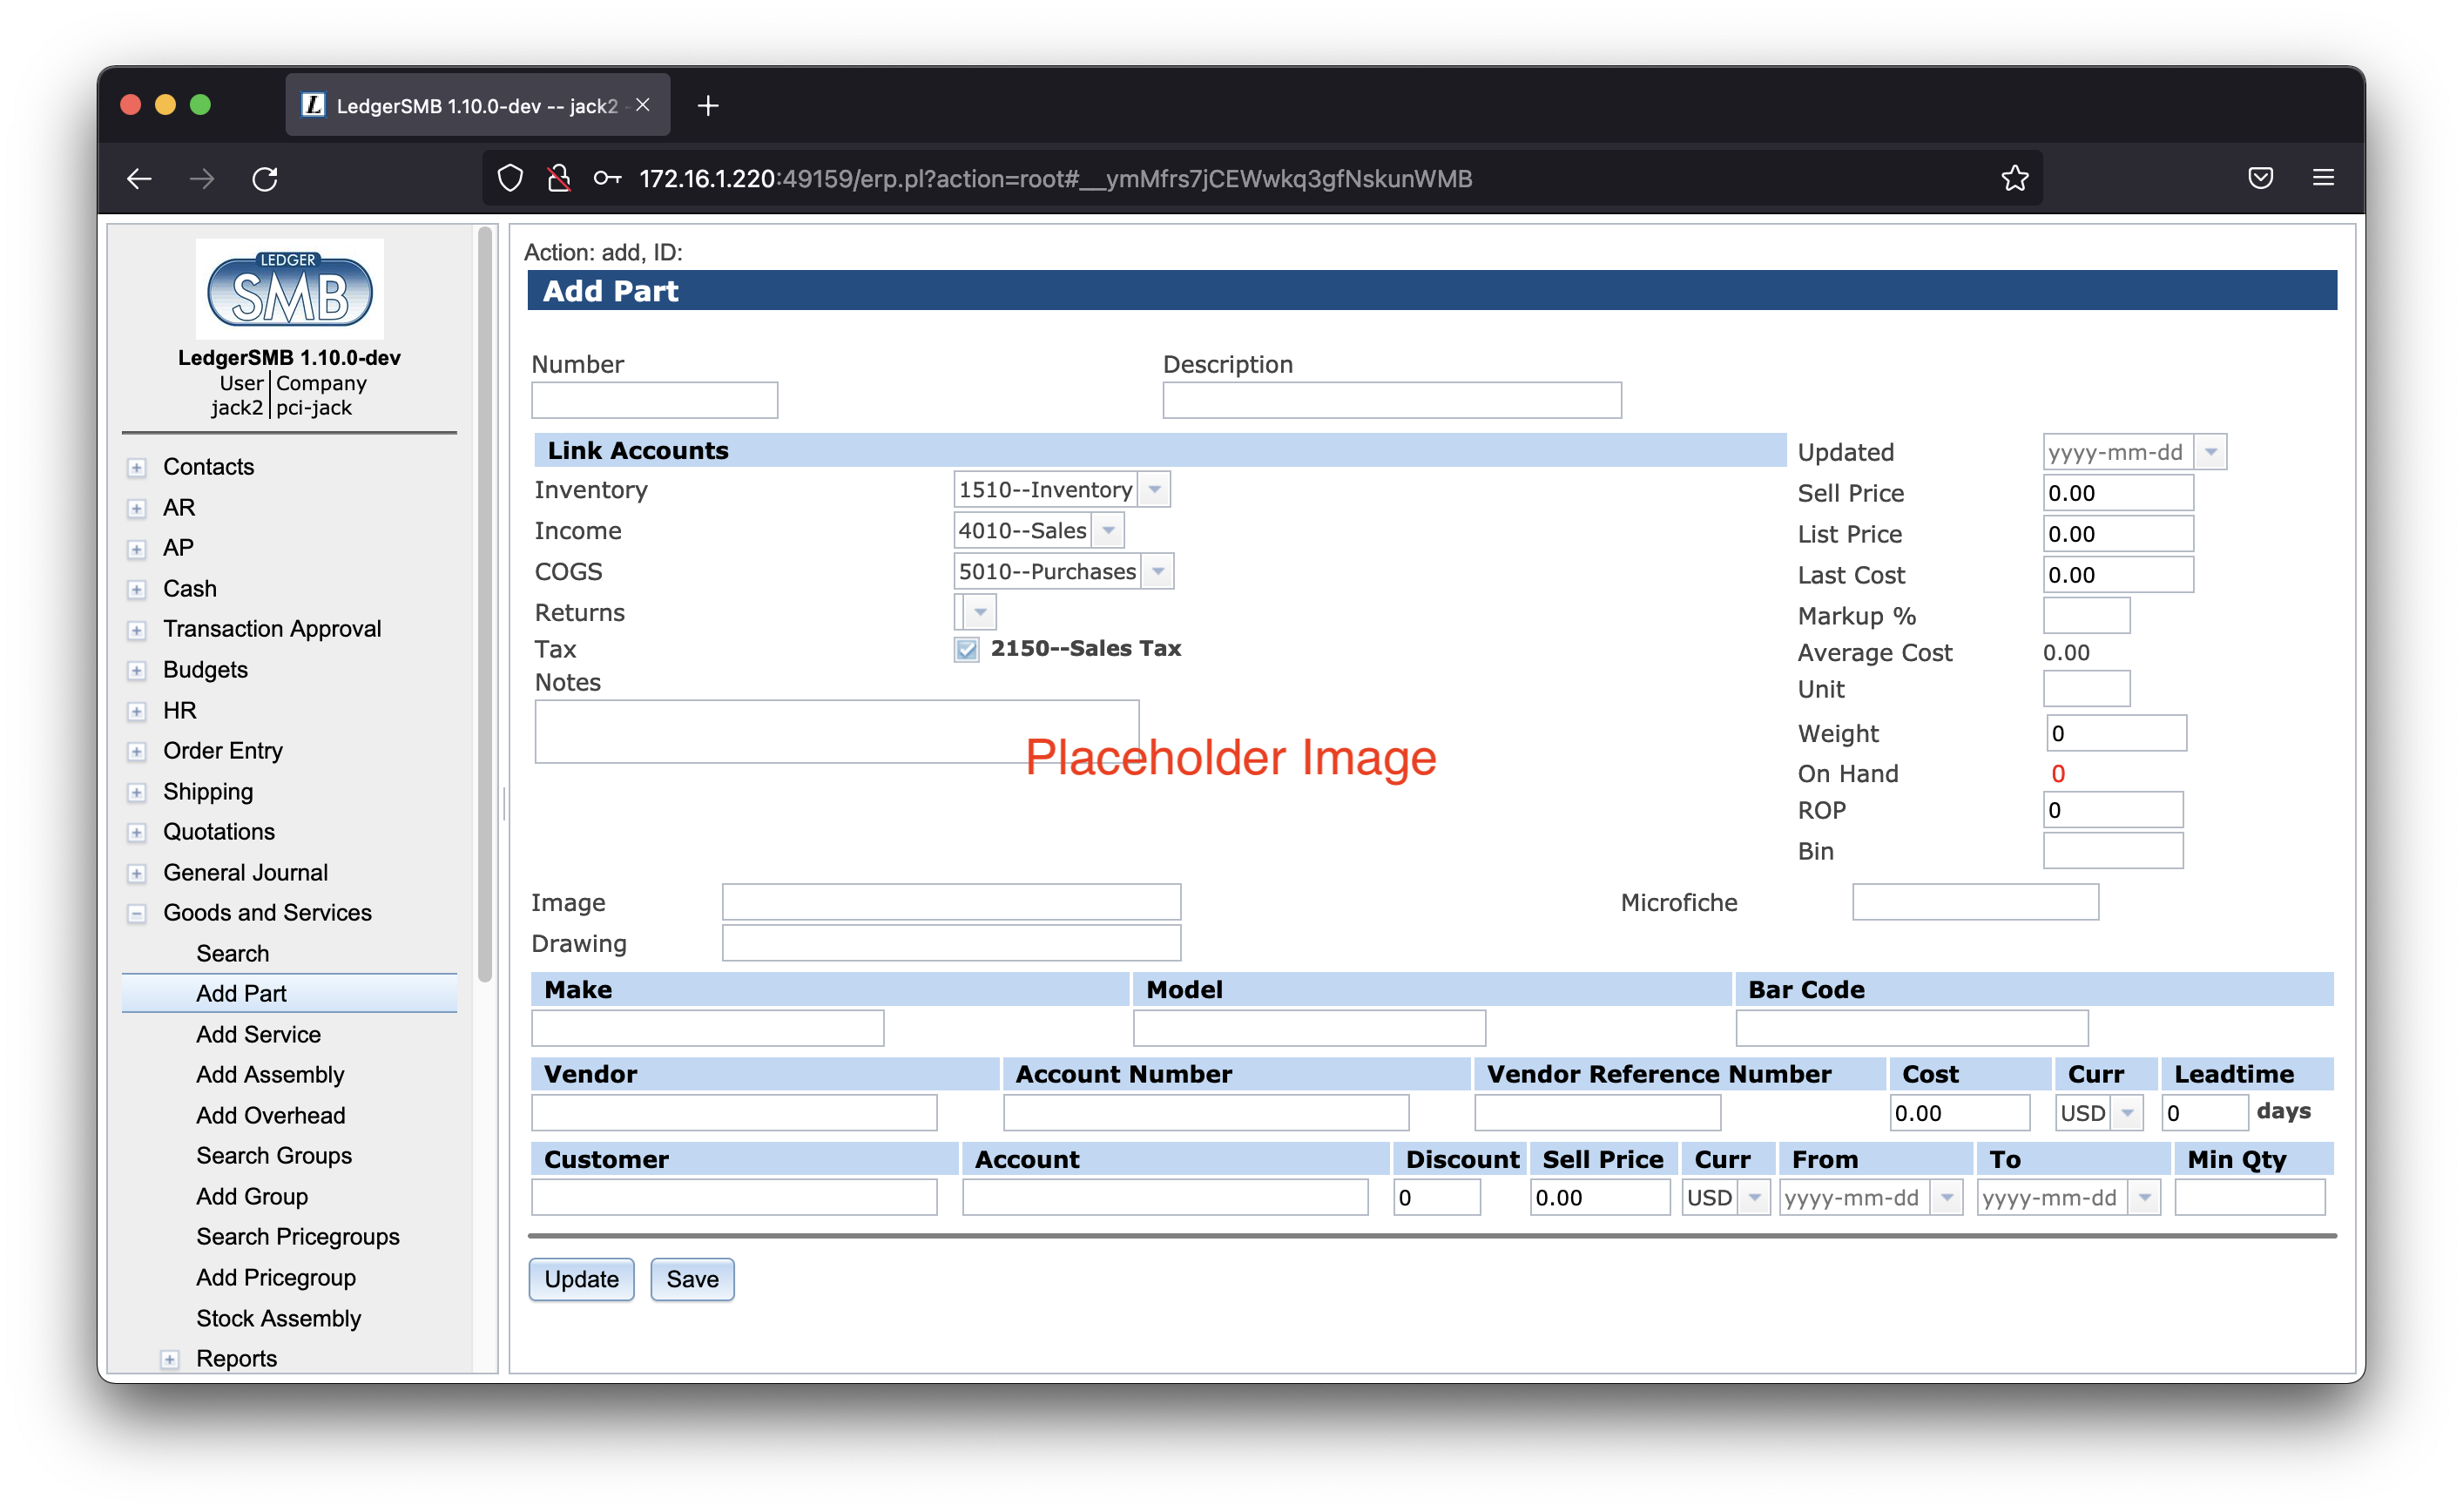
\includegraphics[width=\linewidth]{setup-add-part.png}
        \caption{Add first part}
        \label{fig:setup-add-part}
\end{figure}

Based on his reading from \secref{subsec-products-parts-definition}, Jack decides to enter the hard
drive with the following data:

\begin{tabular}{ll}
Field & Value\\ \hline
Number & \texttt{SAM1TB}\\
Description & \texttt{SAMSUNG 980 PRO 1TB PCIe NVMe Gen4 SSD} \\
Inventory account &  \texttt{1510 - Inventory}\\
Income account &  \texttt{4010 - Sales}\\
COGS account &  \texttt{5010 - Purchases}\\
Sell price &  \texttt{175.00}\\
\\
\end{tabular}

After entering the data Jack clicks \texttt{Save}.

He decides not to include make/model information, drawings or images yet and since
he hasn't entered vendors or customers in his system yet, he decides to leave
those sections blank as well.

\subsection{Combining single-item and ``multi-item pre-packaged'' sales}
\label{subsec-stock-parts-mulit-item}

After having finished setting up the solid state drive, Jack now wants to enter
the memory modules he's going to sell. The problem is that they usually go in pairs,
since that's what the systems consuming them need. However, he expects them to be sold
as single items as well and he wants to be able to set a separate price for those occasions.

From his reading of \secref{subsec-parts-versus-assemblies}, it should be
possible to support this scenario with a small work around\footnote{It's planned to directly
support this use-case in some version higher than 1.3}. From the two solutions available,
he chooses option (b): to create a part and an assembly and regularly restock the assembly
to 0 (zero) in order to remove the stock from the single item.

\section{Defining part groups}
\label{sec-stock-part-groups}

As Jack continues to enter more parts into the system, he wonders how he's going to
look up the parts efficiently later on. Returning his reading to \secref{subsec-products-parts-definition},
he understands that 'part groups' are the solution to that problem. 

He decides to create
the part groups by navigating to:
\begin{quote}
\menupath{Goods and Services \ma Add Group}.
\end{quote}
For each group in the list below Jack enters the group name and clicks \texttt{Save} after each one:

\begin{tabular}{ll}
Field & Value \\ \hline
Group & \texttt{Storage}\\
Group & \texttt{Monitors}\\
Group & \texttt{Input devices}\\
Group & \texttt{Printers}\\
\\
\end{tabular}

After creating these part groups, the ``Group'' drop down appears on the parts entry screen,
allowing him to assign each of his parts to one of these groups.

Since he doesn't expect to be running more than one or two types of CPUs, he decides
not to create a separate group for those and leaves these two parts unassigned.

\section{Defining vendors}
\label{sec-stock-defining-vendors}

Jack selects ``ABC Parts'' to purchase the inventory he needs to run his company. In
order to start buying inventory, ABC Parts needs to be entered as a Vendor to LedgerSMB.

Using the work flow detailed in \secref{sec-workflows-creating-customers-and-vendors} Jack starts to do so by going through the menu \menupath{Contacts \ma Add Contact \ma Company}.
He fills out the Company creation form by clicking the {\tt Generate control code}
button and adding the data as shown in \figref{fig:vendor-create-1}.

\begin{figure}[h]
\centering
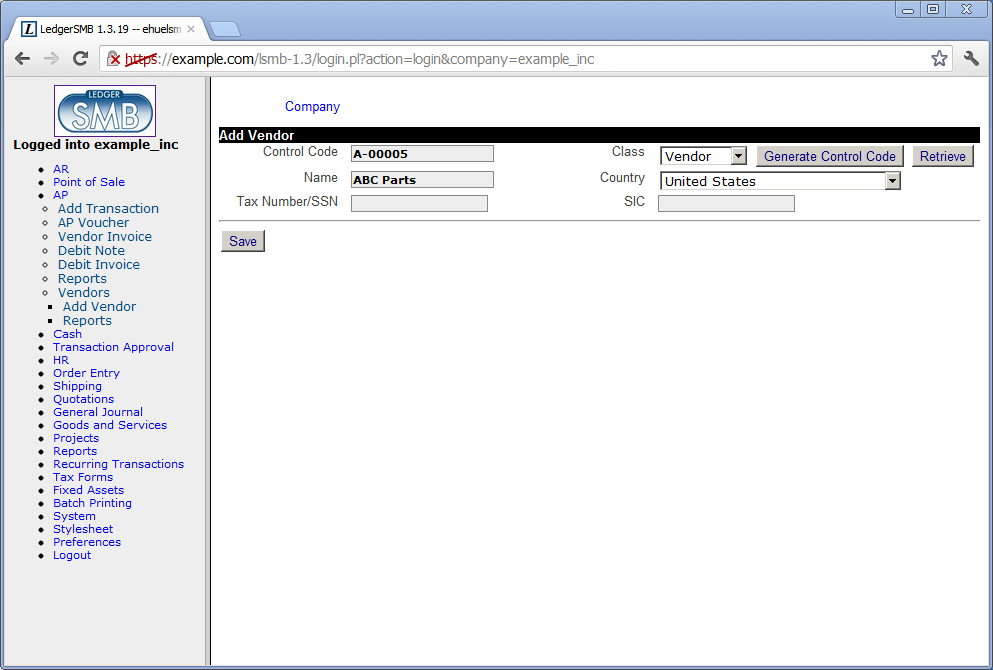
\includegraphics[width=7cm]{bus-vendor-create-2.png}
\caption{Company entry screen}
\label{fig:vendor-create-1}
\end{figure}

After saving the company data, Jack is presented the account data screen which he fills out
as shown in \figref{fig:vendor-create-2}.

\begin{figure}[h]
\centering
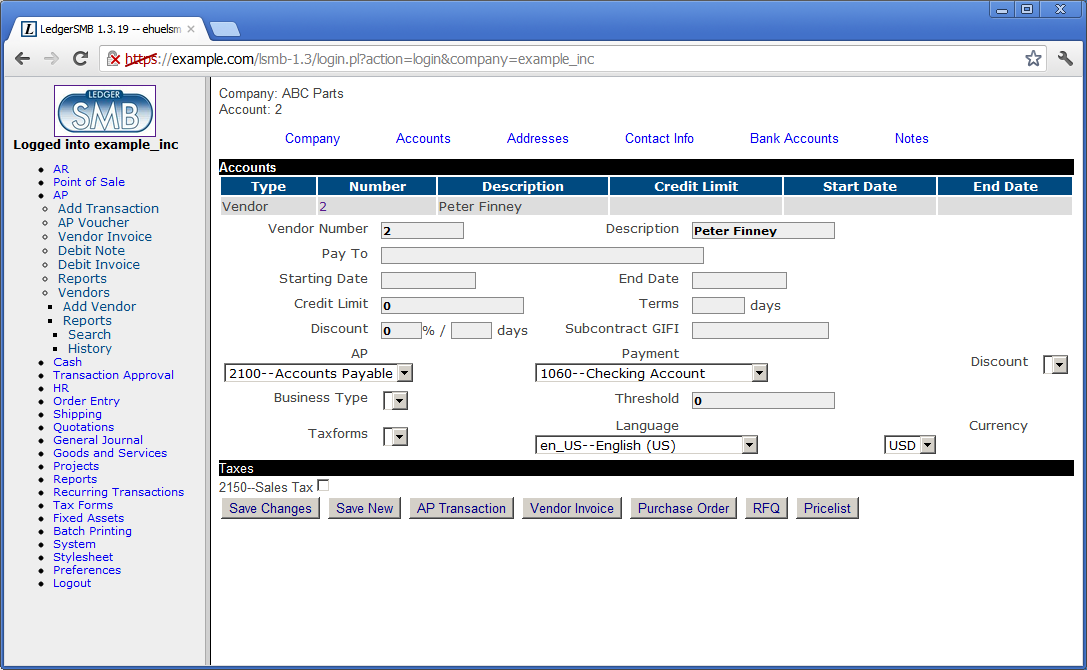
\includegraphics[width=7cm]{bus-vendor-create-3.png}
\caption{Vendor account screen}
\label{fig:vendor-create-2}
\end{figure}

When he's done filling out and saving the form,
he notices the empty ``Discount'' drop down. Reading more about account configuration
check marks in \secref{subsubsec-coa-AR-AP-checkmarks} and going back to the checks on his
chart of accounts (\secref{sec-first-login-coa-check}), he finds he's missing the purchase and
sales discount accounts. He adds two accounts as follows:

\begin{itemize}
\item [4020] Sales discount
\item [5020] Purchase discount
\end{itemize}

After which the page looks like \figref{fig:vendor-create-3}.

\begin{figure}[h]
\centering
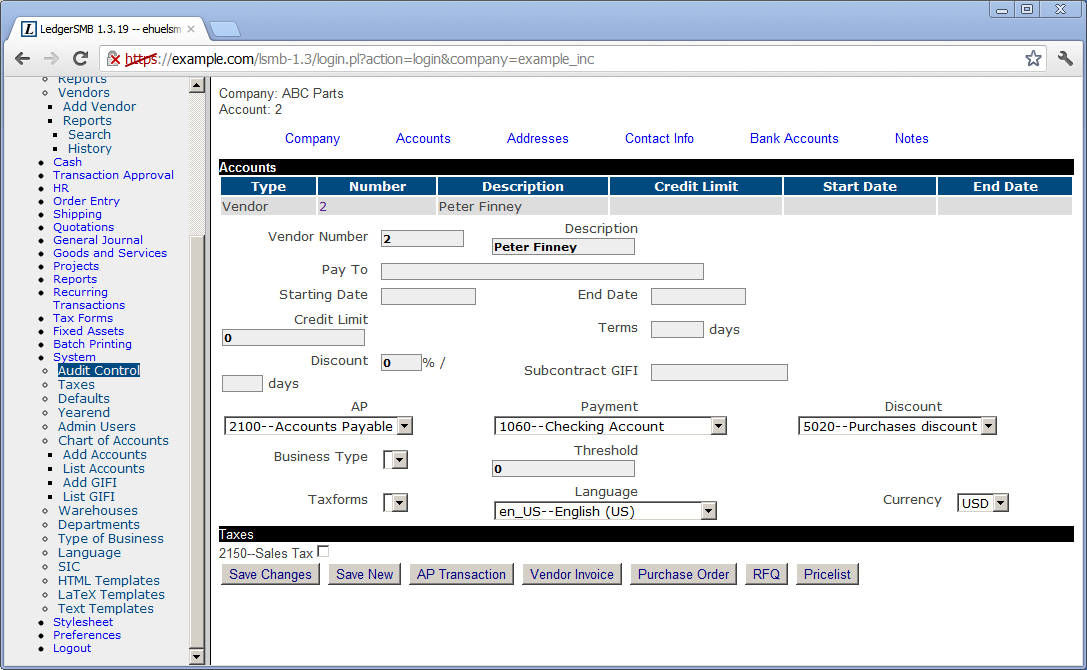
\includegraphics[width=7cm]{bus-vendor-create-4.png}
\caption{Vendor account screen - with purchase discount account}
\label{fig:vendor-create-3}
\end{figure}

Note the top-left corner stating ``Company: ABC Parts'' and ``Account: 2''. The information
entered on the ``Addresses'', ``Contact Info'' and ``Bank Accounts'' tabs will be attached
to the account listed, i.e. account number 2 in this case.

The reader is referred to \secref{sec-workflows-creating-customers-and-vendors} for a more in-depth
description of the vendor data screens.

\section{Requesting quotations}
\label{sec-stock-request-quotation}

After Jack finishes setting up the parts and vendor information, he decides to use LedgerSMB to draw
up a list of items he wants to order from this company. To do so he follows the menu path
\menupath{Quotations \ma RFQ} which opens up a screen (shown
in \figref{fig:rfq-entry-screen}) for entering a new \gls{rfq} .

\begin{figure}[h]
\centering
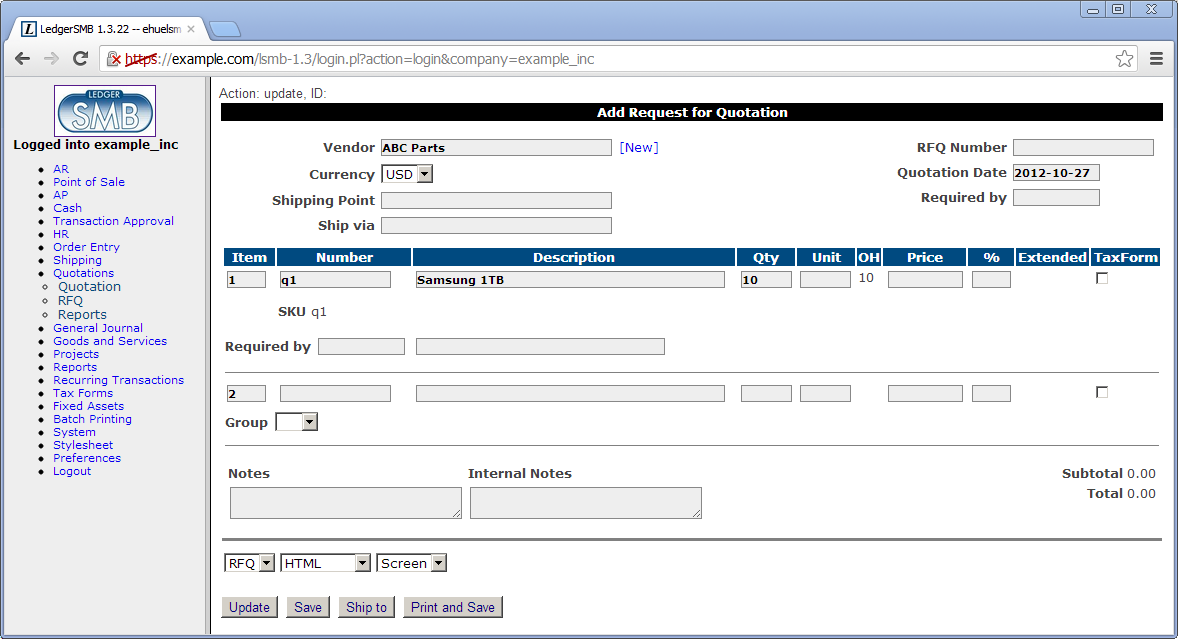
\includegraphics[width=7cm]{rfq-entry-screen.png}
\caption{RFQ entry screen}
\label{fig:bus-rfq-entry-screen}
\end{figure}

\begin{quotation}
\textbf{Remark} Note that the \gls{rfq} entry screen contains prices; this is misleading
at least: the printed output to be sent to the vendor does not. The fact that this screen
allows entry of prices could be considered a bug.
\end{quotation}

After filling out the form in accordance with the description in \secref{sec-workflows-quotations-creation},
Jack expedites his \gls{rfq} to his vendor through e-mail by clicking the ``E-mail'' button. He finds
himself in the screen shown in \figref{fig:rfq-email-screen}.

The From field of the e-mail to be sent out will be filled using the ``Default From'' setting documented
in \secref{subsec-company-config-defaults}. The other address fields can be entered by the user and may be readily
populated if the customer account has the right contact info items attached: if there are Email, Cc and/or
Bcc contact items set up, those will be used to fill these fields.

At the bottom there are three selection lists. The first allows selection of the format used to send the
\gls{rfq}. Available options are HTML, CSV, Postscript (PS) and PDF. The last two require Postscript and PDF
support to be correctly set up. The last selection list selects the language to be used for the
\gls{rfq}. If no value is selected the system default language is used.

\begin{figure}[h]
\centering
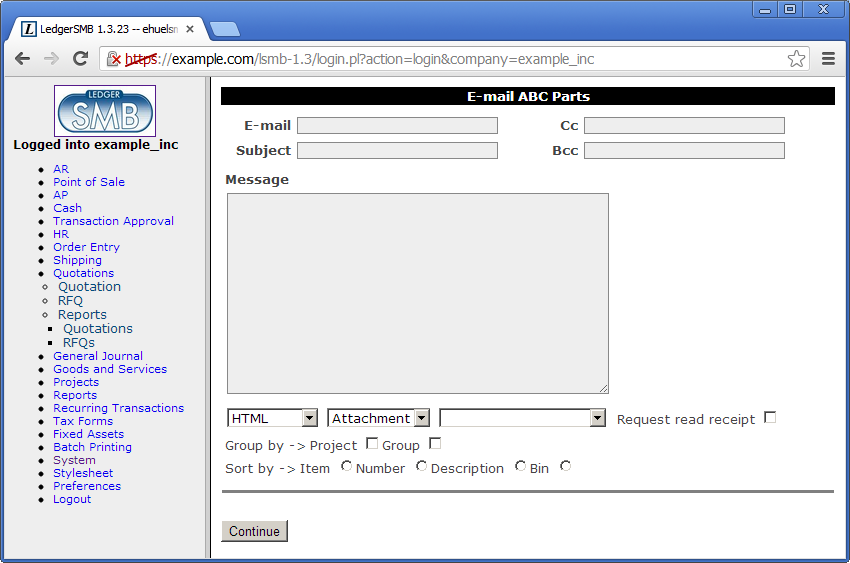
\includegraphics[width=7cm]{rfq-email-screen.png}
\caption{RFQ e-mail screen}
\label{fig:rfq-email-screen}
\end{figure}

For more detail, the reader is referred to \secref{subsec-workflow-quotations-sending-email}.


\section{Following up on a quotation}
\label{sec-stock-quotation-followup}

Jack's vendor (ABC Parts) sends him a quotation in response to his \gls{rfq}. Jack and his vendor
can go back and forth a few times until Jack likes the offer he's getting, but for the sake of
argument let's assume this is the final quotation.

Since Jack likes the offer, he wants to place an order with his vendor. To do so he looks up the
\gls{rfq} he sent to the vendor using the menu path \menupath{Quotations \ma Reports \ma Search}.
The screen shows additional buttons now that it shows a saved RFQ.


\begin{figure}[h]
\centering
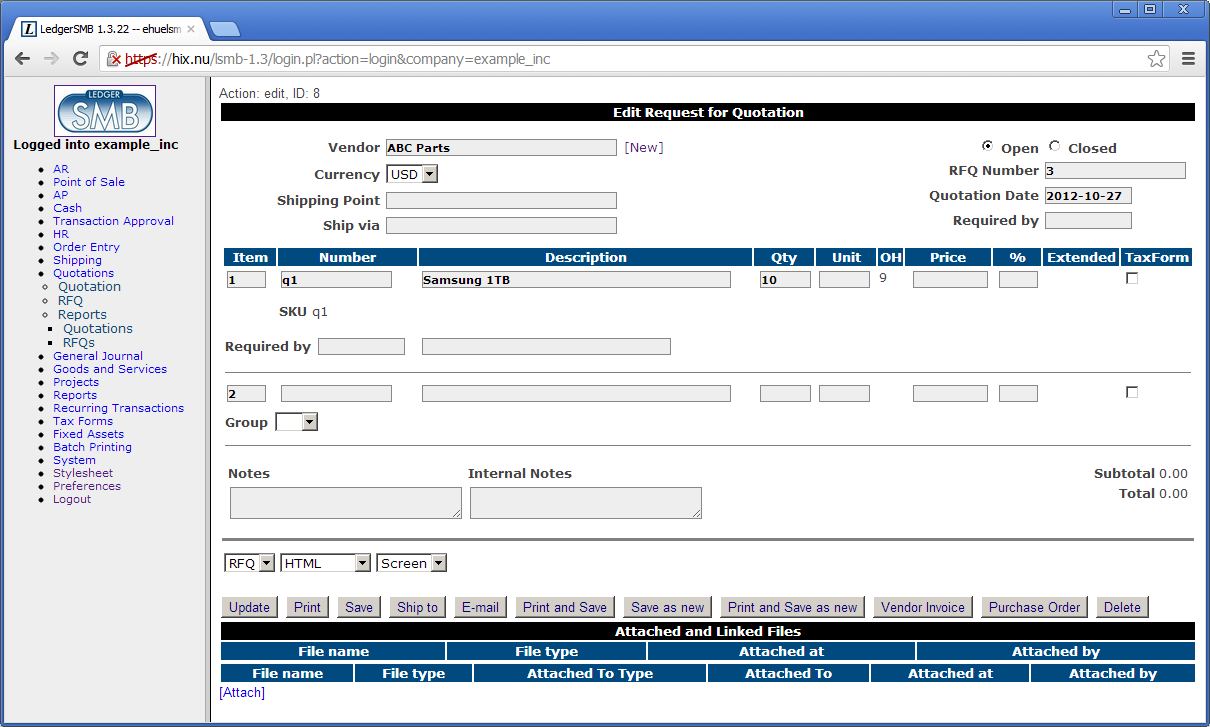
\includegraphics[width=7cm]{rfq-edit-screen.png}
\caption{RFQ entry screen}
\label{fig:bus-rfq-edit-screen}
\end{figure}

Jack clicks the ``Purchase Order'' button which creates a new order from the data in the RFQ.
He completes it
by entering the prices his vendor has quoted and by modifying it to be in accordance with the
quotation. See \secref{sec-workflows-orders-creation-from-quotations} for more
detail on the order entry screen. When finished he saves the order and mails it to
ABC Parts just like he mailed the \gls{rfq} in the previous section.

\figref{fig:purchase-order-screen} shows the screen of a saved purchase order.

\section{Receiving ordered items}
\label{sec-stock-receiving}

Having ordered his inventory, the vendor starts shipping. There's too much to ship at once
so the vendor ships the goods in batches: every week he ships what's available at the end
of that week - he needed to order some of the products with the manufacturer.

LedgerSMB helps Jack keep track to see if he has received everything he has ordered and
that he's not receiving too much. Jack goes through the menus \menupath{Shipping \ma Receive}.
In the search screen, he fills the vendor name (ABC Parts) and clicks ``Continue'' to be listed
all open orders from ABC Parts. By clicking on the order number, the ``Receive Merchandise'' screen
opens as presented in \figref{fig:order-receive-screen}. This allows Jack to handle the incoming
shipment. LedgerSMB will automatically update inventory based on the amounts entered as received
\footnote{To resolve problems in the inventory tracking parts of LedgerSMB (inherited from
before the fork), a significant change has been implemented in 1.3.31: inventory changes won't
be recorded until invoices have been posted.
}.

\begin{figure}[h]
\centering
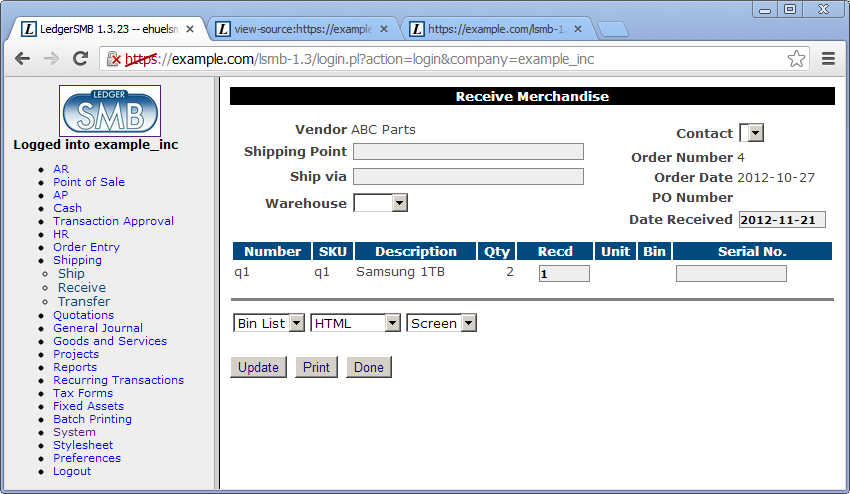
\includegraphics[width=7cm]{order-receive-screen.png}
\caption{Order receipt entry screen}
\label{fig:order-receive-screen}
\end{figure}

\section{Receiving an invoice}
\label{sec-stock-invoice}

\section{Paying an invoice}
\label{sec-stock-payment}



\chapter{Ramping up to the first sale}
\label{cha-ramping-up-to-the-first-sale}

\section{Sending out a quote} 
\label{sec-sending-a-quote}

\section{Sending out a sales order}
\label{sec-sending-a-sales-order}



\chapter{Shipping sales}
\label{cha-shipping-sales}



\chapter{Invoicing}
\label{cha-starting-invoicing}

\section{Handling sales taxes}
\label{sec-invoicing-sales-tax}

\subsection{Invoices with taxes included}
\label{subsec-sales-tax-included}

\subsection{Invoices with explicit tax amounts}
\label{subsec-sales-tax-explicit-amount}

\section{Invoice Editing}
\label{sec-invoicing-editing}

Posted invoices only have 2 fields that can be edited:
\begin{enumerate}
\item Internal notes field
\item Sales person - The Sales Person drop-down is only shown if there are sales people. Sales People are created through Employees and checking the Sales check-mark.
\end{enumerate}
After editing, click the  \texttt{Save Info} button to save the changes.

\chapter{Collecting sales invoice payments}
\label{cha-starting-sales-customer-payments}

\section{Customer payments}
\label{sec-starting-sales-customer-payments}

\section{Customer payment mismatch}
\label{sec-starting-sales-payment-mismatch}

\subsection{Choosing between pardoning and registering underpayment}
\label{subsec-sales-payment-mismatch}

\subsection{Large ones, as in partial payments or largish under/over payments}
\label{subsec-sales-payment-partial}

\subsection{Pardoning small mismatches}
\label{subsec-sales-payment-pardoning}



\chapter{Paying vendor invoices}
\label{cha-starting-vendor-payments}

\section{Handling vendors who match amounts to exact invoices}
\label{sec-vendor-invoice-exact-match}

\section{Handling vendors with running balances}
\label{sec-vendor-invoice-running-balance}

\section{Handling bounced checks}
\label{sec-vendor-invoice-bounced-checks}

\subsection{Voiding checks to undo payments of vendor invoices
 relating to bounced checks}



\chapter{Monitoring arrears}
\label{cha-starting-monitoring-arrears}

\section{Handling interest on arrears}
\label{sec-monitoring-interest-on-arrears}



\chapter{Branching out: services}
\label{cha-starting-branch-to-services}

\section{Creation / assignment to different accounts}
\label{sec-starting-services-assignment}

\section{Recording service hours}
\label{sec-starting-services-writing-hours}

\section{Customer approval on service hours}
\label{sec-starting-services-hours-customer-approval}

\section{Invoicing services}
\label{sec-starting-services-invoicing}

\chapter{Branching out II: service subscriptions}
\label{cha-starting-services-subscriptions}


% !TeX encoding = UTF-8
% !TeX spellcheck = en_US
% !TeX root = ledgersmb-book.tex

\part{Configuration}
\label{part-configuration}


\chapter{Overview}
\label{cha-configuration-overview}

\section{Introduction}
\label{sec-config-overview-introduction}
This section of the book describes how to set up LedgerSMB and its components.
Configuration \index{configuration} is assumed to be mostly one-off and rather technical in nature.  To find
out which tasks might need to be performed in order to keep the application in good
health the reader is referred to the 'Administration Introduction', \secref{sec-administration-introduction}.

\chapter{Global configuration}
\label{cha-global-configuration}

\section{Apache}
\label{sec-global-config-apache}

Section about installing on \index{apache} Apache 2+

items to be discussed:

\begin{description}[style=nextline]
\item [Forwarding of authentication] @@@TODO
\item [PSGI configuration] @@@TODO
\item [performance] cgiD configuration: don't (yet) [but will be supported once all legacy code is gone] @@@TODO
\item [security] suEXEC environment @@@TODO
\end{description}

\subsection{Differences between Apache 1.3 and 2+}
\label{subsec-global-config-apache-13-vs-2}

Explain how to use lsmb with 1.3 instead of 2+.

\section{PostgreSQL}
\label{sec-global-config-postgresql}

\begin{description}[style=nextline]
\item [pg\_hba.conf] authentication @@@TODO \index{pg\_hba.conf}
\item [security] local vs IP connections @@@TODO 
\index{Postgres} \index{Postgres Security}
\end{description}


\section{LedgerSMB version numbers}
\label{sec-global-config-ledgersmb-version-numbers}

LedgerSMB version numbers \index{version number} are in the form of Major.Minor.Patch-Optional Tag. So for example, the current 1.9 development release is \texttt{1.9.28-dev} and the production release is \texttt{1.9.27}

\begin{description}[style=nextline]
\item [Major] An increment in the major release number \index{release number} can mean significant architectural, \gls{API}, functional, or usage changes. It is expected that an upgrade to a new Major version is  going to be planned and tested by the user organization before upgrading.
\item [Minor] An increment in the minor release number may indicate changes to \glspl{API} \index{API}, interfaces, user instructions, etc.  But these changes are not expected to have major impact and should require minor planning and testing. Often small impact enhancements are back-patched to previous Minor versions as patches.
\item [Patch] Increments in the Patch number represent bug fixes, security improvements, or enhancements that do not break existing functionality, usage, or \glspl{API}.  These changes are expected to be applied to an installation as soon as possible.
\item [Optional Tag] Common values include dev, beta, or alpha. Typically, these are only used internally by the LedgerSMB developers.
\end{description}

\section{LedgerSMB Configuration}
\label{sec-global-config-ledgersmb}

LedgerSMB configuration using \texttt{ledgersmb.conf} \index{ledgersmb.conf} is deprecated as of 1 Jan 2023. New functionality may only available when using \texttt{ledgersmb.yaml} \index{ledgersmb.yaml} configuration file.

For the time being there is a conversion step that converts the old 'ledgersmb.conf' to `ledgersmb.yaml`, but the old conf file does not support new functionality.

\subsection{ledgersmb.yaml}
\label{subsec-global-config-ledgersmb-yaml}

For an example of the default, non debug \texttt{ledgersmb.yaml} \index{ledgersmb.yaml} see  \url{https://github.com/ledgersmb/LedgerSMB/blob/master/doc/conf/ledgersmb.yaml}

\subsubsection{\texttt{cookie}}
 @@@TODO

\subsubsection{\texttt{db}}
 @@@TODO

\subsubsection{\texttt{default\_locale}}
@@@TODO

\subsubsection{\texttt{environment\_variables}}
 @@@TODO

\subsubsection{\texttt{extra\_middleware}}
@@@TODO

\subsubsection{\texttt{logging}}
@@@TODO

\subsubsection{\texttt{login\_settings}}
@@@TODO

\subsubsection{\texttt{mail}}

Email \index{mail} can be configured by selecting which of the three available transports to use. The default \texttt{ledgersmb.yaml} file contains examples for the first two.

\begin{description}
    
    \item{\texttt{Email::Sender::Transport::Sendmail}} – Emails are sent using the local server's \texttt{sendmail} \index{sendmail} binary. The configuration parameters are:
    \begin{description}
        \item{\texttt{transport:\$class}} – \texttt{Email::Sender::Transport::Sendmail}
        \item{\texttt{transport:path}} – optionally provide a path to the directory that contains the 'sendmail' binary.
    \end{description}
    
    \item{\texttt{LedgerSMB::Mailer::TransportSMTP}} - Emails \index{email} are sent using a remote SMTP \index{SMTP} server.  The configuration parameters are:
    \begin{description}
        \item{\texttt{transport:\$class}} – \texttt{LedgerSMB::Mailer::TransportSMTP}
        \item {\texttt{transport:host}} – The required host name of the smtp \index{ SMTP} server.
        \item {\texttt{transport:port}} – The required port number of the smtp server. Note this might vary depending on whether TLS or SSL is used.
        \item {\texttt{sasl\_username:\$class}} – The required smtp server authentication method. The values can be `Authen::SASL` or `Authen::SASL::SCRAM`.
        \item {\texttt{sasl\_username:mechanism}} –  The available mechanism are defined at \url{https://metacpan.org/dist/Authen-SASL} or \url{ https://metacpan.org/dist/Authen-SASL-SCRAM} depending on the selected `\$class`.
        \item {\texttt{sasl\_username:callback:user}} – The required SMTP user name.   'the-user' in the default file is a place holder and must be replaced.
        \item {\texttt{sasl\_username:callback:pass}} – The required SMTP password.  'SECURITY-FIRST' in the default file is a place holder and must be replaced.
    \end{description}
    
    \item{\texttt{Email::Sender::Transport::DevNull}} -  Emails are sent to \texttt{/dev/null}, in other words emails are not sent anyplace. This prevents errors in the user interface, but throws away any mail.  There is only one configuration parameter.  This is not a recommended production configuration. It is usually used for testing.
    \begin{description}
        \item{\texttt{transport:\$class}} – \texttt{Email::Sender::Transport::DevNull}
    \end{description}

\end{description}

\subsubsection{\texttt{miscellaneous}}
@@@TODO

\subsubsection{\texttt{output\_formatter}}
@@@TODO  I really don't have a good way to format lists explanations.  See below at \texttt{paths:config:workflows} for an example. Guidance welcome.

\subsubsection{\texttt{paths}}

This section configures the various paths used by LedgerSMB. The configuration parameters are:

\begin{description}
    \item {\texttt{config:locale}} – Path to locale \index{locale path} files. Defaults to \texttt{locale/po}.
    \item {\texttt{config:sql}} – Path to the SQL schema \index{SQL schema path} definition files. 
    \item {\texttt{config:sql\_data}} – Path to the reference and initial SQL database load \index{database load path} files. For example, the names of the countries.
    \item {\texttt{config:templates}} – Path to the templates \index{template path} base directory. Typically set to \texttt{templates}.
    \item {\texttt{config:UI}} – Path to the UI HTML \index{HTML path} files. Defaults to \texttt{./UI/}
    \item {\texttt{config:UI\_cache}} – Path to the location of the UI template cache \index{template cache path}. These are cached after they have been parsed and translated. This improves performance.
    \item {\texttt{config:workflows}} – A list of the Directories where workflow files \index{workflow path} are stored. Contains the default and custom workflows.  Custom workflows are used to override behavior of the default workflows by providing actions, conditions, etc. with the same name and type or by providing workflows of the same type with additional states and actions. Default workflows defaults to \texttt{workflows}. Custom workflows defaults to \texttt{custom\_workflows}. Default workflow path must precede all the custom workflow paths. @@@TODO is the last statement correct?  Can there be more than 2 paths?
\end{description}

\subsubsection{\texttt{printers}}
This section contains a list of printers \index{printing} and their definition.

The default  \texttt{ledgersmb.yaml} file shows two printers \index{printer configuration} named 'Laser' and 'Epson' with the printers defined using the linux \texttt{lpr} command and its arguments. 

This default definition will provide for the selection of the printers named  'Laser' and 'Epson' in the LedgerSMB user interface.

For more information search the internet for 'linux lpr command' or use \texttt{man lpr} at the linux command line.

\subsubsection{\texttt{reconciliation\_importer}}
 @@@TODO

\subsubsection{\texttt{setup\_settings}}
@@@TODO

\subsubsection{\texttt{ui}}
@@@TODO

\subsubsection{\texttt{workflows}}
@@@TODO

\chapter{Per company configuration}
\label{cha-company-config}

\section{Matching your business processes}
\label{sec-company-config-matching-your-business}

By default, LedgerSMB operates such that all optional functionality is available and the user decides to use it or not based on which menu items they select, what fields they enter data into, and what buttons they click.

Removing application roles \index{application roles} (see \appref{app-role-listing}) can limit the visibility of  menu items, data fields, and buttons. This will simplify the users view of the system, reduce training, and better configure LedgerSMB to your business requirements.

Outside of application roles, the only other enforced business process configuration is whether the same person can both create and post transactions. It is called 'separation of duties' \index{separation of duties} and is defined in \secref{subsubsec-company-config-defaults-separation-of-duties}.

LedgerSMB is configured to adjust inventory \index{inventory} when a Sales or Purchase Invoice is posted. This closely matches retail business processes where the customer walks out of the establishment with the product and an invoice \index{invoice} (or receipt).  This functionality can also be used for wholesale shipping applications because LedgerSMB can also produce picking \index{picking} and \index{shipping} shipping documents, just remember that the inventory transaction happens when an invoice is posted.

LedgerSMB uses \gls{FIFO} \index{FIFO} for \gls{COGS} \index{COGS} and inventory calculations.  There are provisions for alternatives, but the code is not yet complete. See \secref{sec-accounting-valuation-inventory} for a detailed explanation of  \gls{FIFO} calculations.

In addition to the above, LedgerSMB has configurable Workflows \index{workflows}. These are not user configurable but your technical support staff should be able to create and edit them. See \charef{part-workflows}.

Contact the \href{https://ledgersmb.org}{development team} for other business process customizations.  In most cases the need for more flexible matching of LedgerSMB to your business processes is understood, but the project has not not yet had any customer requests or development volunteers.

\section{Administrative user}
\label{sec-company-config-admin-user}

\section{Chart of accounts}
\label{sec-company-config-coa}

@@@ Should refer to the 'administration' section???

\subsection{Special accounts}
\label{subsec-company-config-coa-special-accounts}

\begin{itemize}
\item AR/AP summary accounts
\item 5 other special purpose accounts, see ``Defaults'' screen discussion
\item sales tax accounts
\end{itemize}


\section{System menu settings}
\label{sec-company-config-system-menu}

This section enumerates the ``System'' menu's immediate children. In some cases the
functionality is too complex and is referred to a chapter of its own.

\subsection{Audit control}
\label{subsec-company-config-audit-control}

\subsubsection{Enforce transaction reversal for all dates}
\label{subsubsec-company-config-audit-control-reversals}


This is a Yes/No value which affects the actions which can be performed on posted financial transactions.
\begin{itemize}
\item No means transactions can be altered or deleted, even after posting them. Note that
if a transaction has been posted before the latest closing date, it can never be altered,
not even when this value is in effect.
\item Yes means transactions can't be altered after posting. This setting is highly preferred and considered the only correct approach to accounting as it assures visible
audit trails and thereby supports fraud detection.
\end{itemize}

\subsubsection{Close books up to}
\label{subsubsec-company-config-audit-control-close-books}


@@@ This item isn't a system setting; shouldn't it move to ``Transaction approval''?? That way system settings (config) and processes are separated.

@@@ My preference is to remove the setting entirely and rely on year-end 
workflow.  We might add an account checkpoint interface as well at some point
--Chris T

It's advisable to regularly close the books after review. This prevents user error changing
reviewed numbers: after closing the books, it's no longer possible to post in the closed
period.

There are also performance benefits to closing the books, because LedgerSMB uses the
fact that the figures are known-stable as a performance optimization when calculating
account balances.

\subsubsection{Activate audit trail}
\label{subsubsec-company-config-audit-control-audit-trail}

This is a Yes/No value which - when Yes - causes the system to install triggers to register
user actions (creation/adjustments/reversals/etc...) executed on financial transactions.


@@@ Once activated, where can we see it the audit trail??

@@@ This setting should go.  In 1.3 the audit trails are always enforced via
triggers so this setting does nothing.  --CT

\subsection{Taxes}
\label{subsec-company-config-taxes}


This page lists all accounts which have the ``Tax'' account option enabled as discussed in \secref{sec-coa-account-options}.

Each account is listed at least once, but can be listed many times, if it has had different
settings applied over different time periods. E.g. if one of the current VAT rates is 19\%,
today but it used to be 17.5\% until last month, there will be 2 rows for the applicable
VAT account. See \charef{cha-taxes} for further discussion of how taxes work in
LedgerSMB and the choices involved when being required to handle changes in tax rates.

Each row lists the following fields:

\begin{description}[style=nextline]
\item [Rate (\%)] The tax rate to be applied when calculating VAT to be posted on this account.
\item [Number] Account number
\item [Valid To] The ending date of the settings in this row. This can apply to the rate as well as the ordering or the tax rules (but usually applies to the rate).
\item [Ordering] This has to do with cumulative taxes.  For example if two taxes
exist and one has an ordering of 0 and one of 1, then the second tax will be
calculated on a basis that includes the first.  One place where this used to be
used was in Quebec, where GST was taxable under PST.
\item [Tax rules] LedgerSMB features a flexible structure to facilitate complex tax
calculations (see \secref{sec-tax-rule-plugins}). By default the ``Simple'' module
is the only one installed.
\end{description}

\subsection{Defaults}
\label{subsec-company-config-defaults}

\subsubsection{Business number}
\label{subsubsec-company-config-defaults-business-number}
   This is used to store an arbitrary identification number for the business.  It
could be used to store a business license number or anything similar.
   
\subsubsection{Weight unit}
\label{subsubsec-company-config-defaults-weight-unit}
   The unit of measurement for weights. @@@ why don't we have a unit of measurement for distance as well??? And maybe a unit of measurement for content?
   
\subsubsection{Separation of duties}
\label{subsubsec-company-config-defaults-separation-of-duties}

% For better or worse this is the spot for the canonical definition of separation of duties.

Separation of duties \index{separation of duties} is a method to help reduce fraud where one employee can't modify the
accounting ledger without another employee's approval.

Select "Yes" if you want to activate separation of duties or "No" if you don't
want to activate it.

In order for separation of duties to be enforced, user roles have to be set differently for each user. This is done by removing the \texttt{draft\_post} role from the users that cannot post and making sure that the users that can post have the role enabled.  See \secref{sec-user-management-authorization} for more details about changing and setting User Roles.

\subsubsection{Default accounts}
\label{subsubsec-company-config-defaults-accounts}

This setting will be used to preselect an account in
the listings of the three categories listed below:
\begin{itemize}
\item Inventory
\item Income
\item Expense
\end{itemize}


\subsubsection{Foreign exchange gain and loss accounts}
\label{subsubsec-company-config-defaults-fx-accounts}

When working with foreign currencies,
the system needs two special purpose accounts. One to post the gains onto which are
caused by foreign currencies increasing in value; the other to post the losses onto
which are caused by foreign currencies decreasing in value.


\subsubsection{Default country}
\label{subsubsec-company-config-defaults-country}

This setting indicates which country needs to be pre-selected
   in country selection lists.


\subsubsection{Default language}
\label{subsubsec-company-config-defaults-language}

The language to be used when no other language has been selected. Several parts of the
application require language selection, such as customer, vendor and employee entry screens.

\subsubsection{Templates directory}
\label{subsubsec-company-config-defaults-templates}

This setting indicates which set of templates - stored in the
   \texttt{templates/} directory - should be used. In a standard installation, the drop down
   lists two items:
\begin{description}[style=nextline]
   \item [demo] which contains templates based on \LaTeX, which is more commonly installed but has issues dealing with accented characters
   \end{description}


\subsubsection{List of currencies \& default currency}
\label{subsubsec-company-config-defaults-currencies}

Enter a list of all currencies you want
to use in your company, identified by their 3-letter codes separated by a colon; i.e.
``USD:EUR:CHF''. To ensure correct operation of the application, at least one currency
(the company default currency) must be listed. In case of multiple currencies the first
is used as the company default currency.

\subsubsection{Company data (name /address)}
\label{subsubsec-company-config-defaults-name-address}

The fields ``Company Name'', ``Company Address'',
``Company Phone'' and ``Company Fax'' will be used on printed/e-mailed invoices.

\subsubsection{Password duration}
\label{subsubsec-company-config-defaults-password-duration}

This is an integer value field measuring the validity period in days for passwords set through
the user's \texttt{Preferences} screen. If this field is empty, passwords set through that method
won't expire.

The user has to log into LedgerSMB after this field is changed and prior to the expiration of the previous setting in order for the new duration to take effect.

A user will receive password \index{password duration} expiration reminders upon logging starting a week before password
expiry. When not acted upon, starting two days before expiry an hourly popup will appear
requesting the user to change the password.

The application behaves this way because users with expired passwords won't be able to log in:
their password will need to be reset by a user admin.

\begin{quote}
Note that passwords set by admins for other users expire \index{password expiration} within 24 hours after setting them.
This value is hard coded and can't be overruled. This is a security measure taken to make
sure as few unused accounts as possible exist: Existence of such accounts could open up security
holes.
\end{quote}


\subsubsection{Default E-mail addresses}
\label{subsubsec-company-config-defaults-email}

These addresses will be used to send e-mails \index{email} from the system.
Note that the ``Default Email From'' address should be configured in order to make sure
e-mail doesn't look like it's coming from your webserver. The format to be used is \texttt{``Name'' <e-mail address>} where the e-mail address should be inserted between the
``$\langle$'' and ``$\rangle$''.

\subsubsection{Max per dropdown}
\label{subsubsec-company-config-defaults-max-dropdown}

Some elements in the screens may present a drop down. However, drop downs are
relatively unwieldy to work with when used to present a large number of values
to choose from.

This configuration option sets an upper limit on the number of records to be
presented as drop down.  When the number is exceeded, no drop down is used.  Instead,
a multi-step selection procedure will be used.

\subsubsection{Item numbering}
\label{subsubsec-company-config-defaults-item-numbers}

Many items in the system have sequence numbers: invoices, parts, etc.
These \index{sequence numbers} can be just a number (i.e. 1 or 37) or
they can also be both prefixed and suffixed. For example, INV0001 for invoices and EMP001 for employees or YOU-0001TOO, in which case the next item will be YOU-0002TOO. 

You can only issue every number in the sequence once, but you can issue Y21-001 and Y22-001 by changing the sequence number format at the beginning of the year.

The numbers shown in the input boxes will be used to generate the next number in the
numbering sequence.

\begin{description}[style=nextline]
\item [GL Reference number] The default reference number for the next GL transaction.
\item [Sales invoice/ AR Transaction number] This number is used to generate an invoice
number when none is being filled out by the user.
\item [Sales order number ] Same as Sales invoice number, except that it's used for sales orders @@@ layout issue: the label is too big to fit on the page
\item [Vendor invoice/ AP Transaction number] Same as Sales invoice, except that the number
is used for accounts payable transactions. @@@ layout issue: the label is too big to fit on the page 
\item [Sales quotation number] Same as sales order number, except that it's used for quotations.
\item [RFQ number] Request for quotation number is like the sales quotation number, except
that it is used to track which vendors have been asked for quotes.
\item [Part number] All parts, services and assemblies are identified by a unique number.
When an item is created and no number is entered by the user, a number is generated
from this sequence.
\item [Job/project number] Used when creating new projects.
\item [Employee number ] Same as the sales invoice number, used by new employee entry.
\item [Customer number] @@@ is this the control code number? or is this
meta\_number?? -- Meta-number (CT) 
\item [Vendor number] @@@ same question as customer number
\end{description}

\subsubsection{Check prefix}
\label{subsubsec-company-config-defaults-check-prefix}

 The prefix to use when printing checks. There's no check sequence number. That sequence number is requested from the check printing interface, because
checks can be created outside the application as well, meaning the numbers can
get out of sync.

\subsection{Year end}
\label{subsec-company-config-year-end}

@@@ Rename ``Yearend'' in menu interface to ``Year end''.


@@@ IMO this section doesn't belong here, because it's a process, not config, but does it belong in this menu then? IMO it doesn't...


\subsection{Admin users}
\label{subsec-company-config-admin-users}

@@@ Same as Year end; doesn't belong here...

\subsection{Chart of accounts}
\label{subsec-company-config-coa}

@@@ Chart of accounts isn't exactly a ``process'', but it doesn't feel like being pure
config either. At any rate it's a fact that the CoA discussion is a full chapter in and
of itself - so discussion here isn't necessary anymore.

\subsection{Warehouses}
\label{subsec-company-config-warehouses}

Warehouses are stocking locations. They don't have any properties (in the system)
other than that they have a name. Warehouses can be added, modified and deleted from
the \menupath{System \ma Warehouses} menu item.

\subsection{Departments}
\label{subsec-company-config-departments}

Departments can be used to divide a company in smaller pieces. LedgerSMB distinguishes two
types of departments:

\begin{description}[style=nextline]
\item [Profit centers] which can be associated with any type of transaction, including AR transactions.
\item [Cost centers] which can be associated with all types of transactions, except AR transactions.
\end{description}

Departments can be created (added), modified or deleted through the \menupath{System \ma Departments} menu item.

\subsection{Type of business}
\label{subsec-company-config-business-types}

Types of business are used in sales operations where customers can be assigned a type
of business. Based on the type of business assignment, quotations, sales orders and
invoices will automatically apply discount rates. For each type of business you enter a description and a discount rate to be applied.

\subsection{Languages}
\label{subsec-company-config-languages}

The language table is the table users can select languages from, both to present
the UI of the application as well as the setting for customers to be used to generate
documents.

This listing should correspond to the actual translations of the application being
available in the program installation directory.

Languages can be added, modified or deleted through the \menupath{System \ma Language} menu item.

\subsection{Standard Industry Code (SIC)}
\label{subsec-company-config-sic}

SI codes feature these three fields:

\begin{description}
\item [Code]
\item [Heading]
\item [Description]
\end{description}

When creating a company you can assign that it an SIC code, irrespective of its role (i.e. customer,
vendor, lead or anything else). An example of an SI code system is the
US's NAICS\footnote{\url{https://www.census.gov/naics/}} code.
Other countries have their own coding systems such
as ANZSIC\footnote{\url{https://www.abs.gov.au/statistics/classifications/australian-and-new-zealand-standard-industrial-classification-anzsic/latest-release}} for Australia and New Zealand
and NACE\footnote{\url{https://ec.europa.eu/competition/mergers/cases/index/nace\_all.html}} for Europe

The SIC field currently doesn't support a specific function in the application and is there
merely for informational purposes. However in the future its role could be extended to include
impact on reports, taxes or other functionalities where type of industry could matter.

\subsection {Templates}
\label{subsec-company-config-templates}

Templates are available to control the output format of many LedgerSMB outputs including Balance Sheet, Sales Orders, etc.

There are 3 types of templates: \LaTeX, HTML, and CSV.
Templates are accessed by navigating to \menupath{System \ma Templates}.
You should see the view shown in \figref{fig:system-templates}.

The template you want to change is selected in the "Template" drop-down. The template format you want to change is selected in the "Format" drop-down.

\begin{figure}[h]
        \centering
        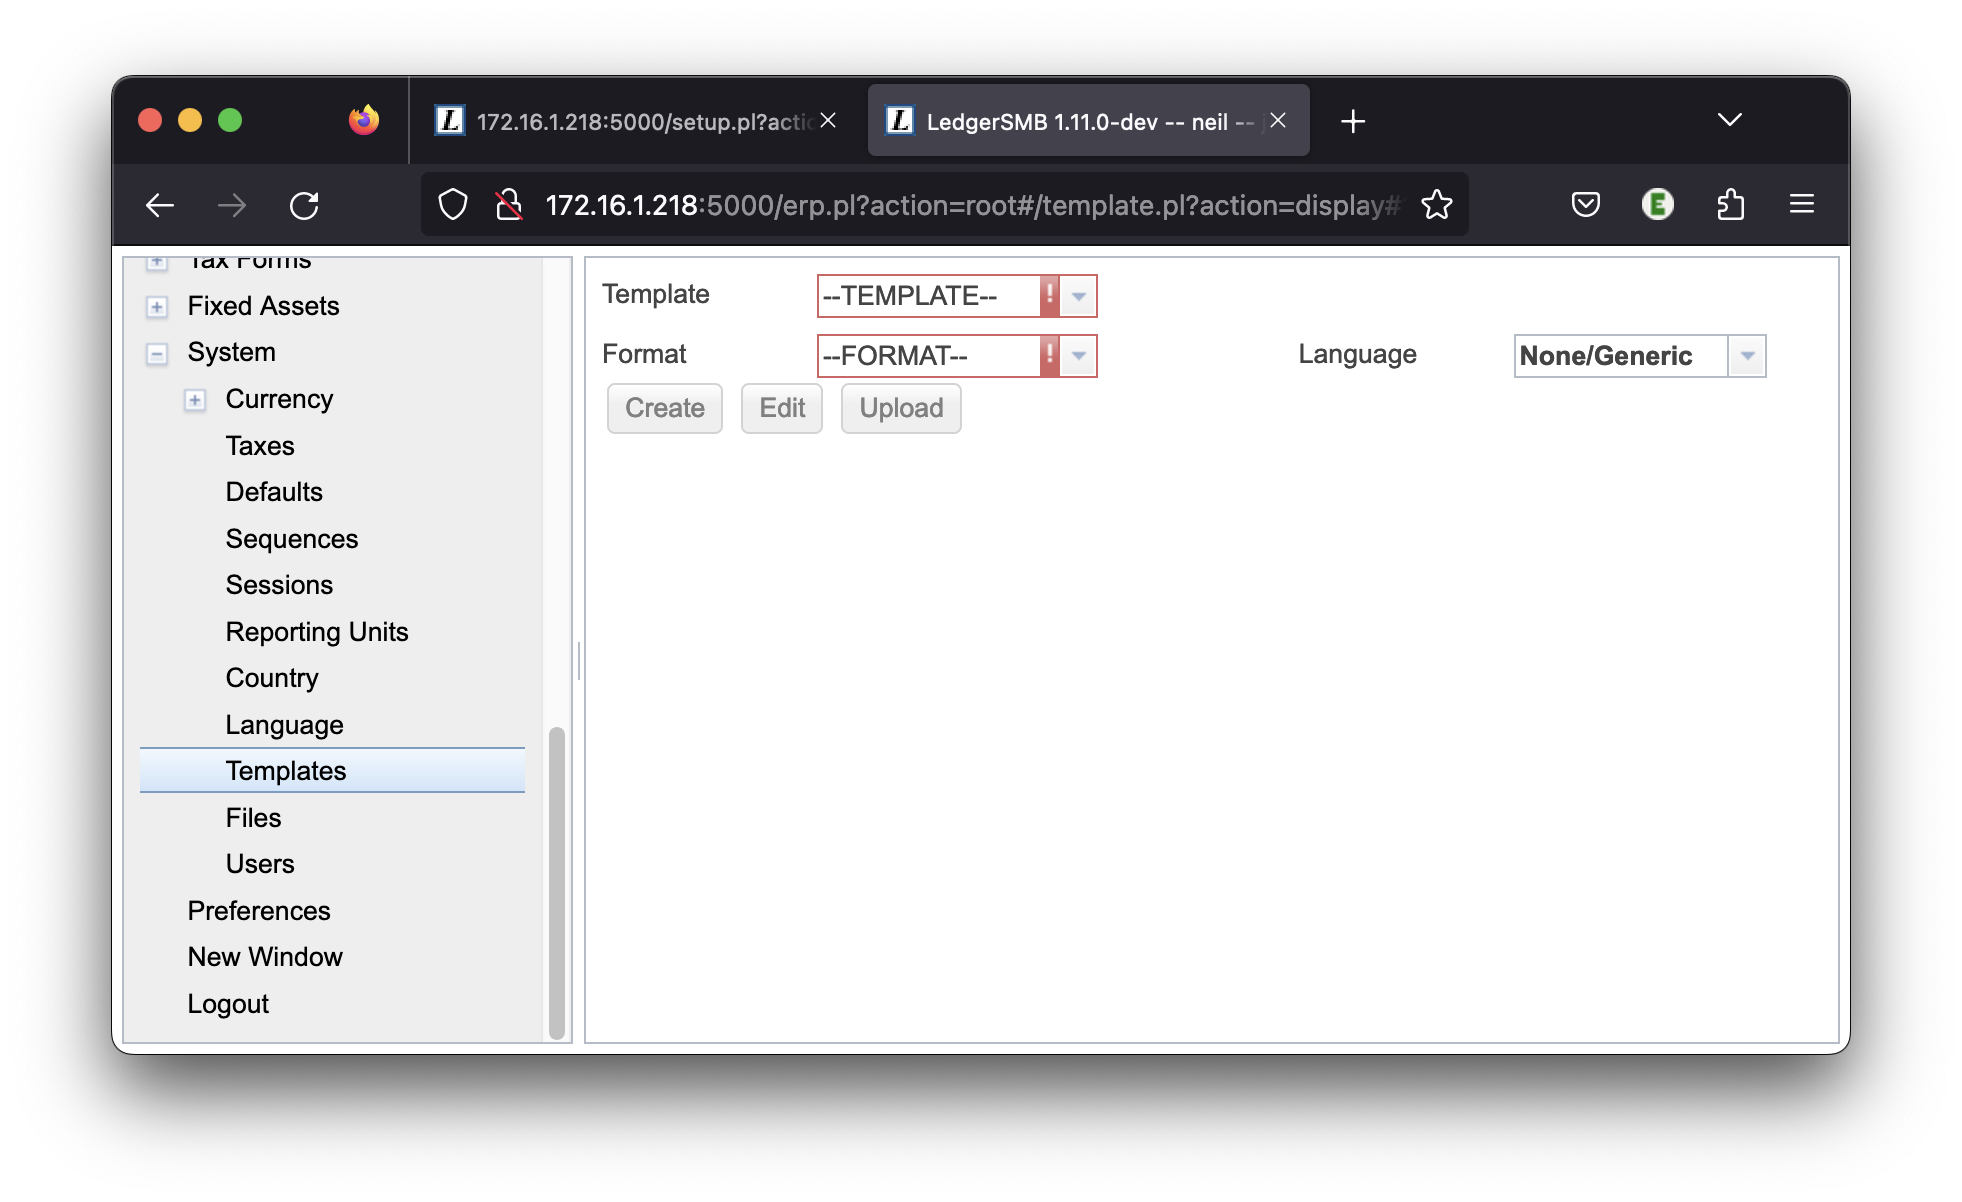
\includegraphics[width=\linewidth]{system-templates.png}
        \caption{System templates screen}
        \label{fig:system-templates}
\end{figure}

\subsubsection{\LaTeX{} templates}
\label{subsec-company-config-latex-templates}

To change a \LaTeX{} template navigate to \menupath{System \ma Templates}.
Select, for example, Template "Invoice" and Format "tex", you should see the view shown in \figref{fig:system-templates-edit-invoice}

\begin{figure}[h]
        \centering
        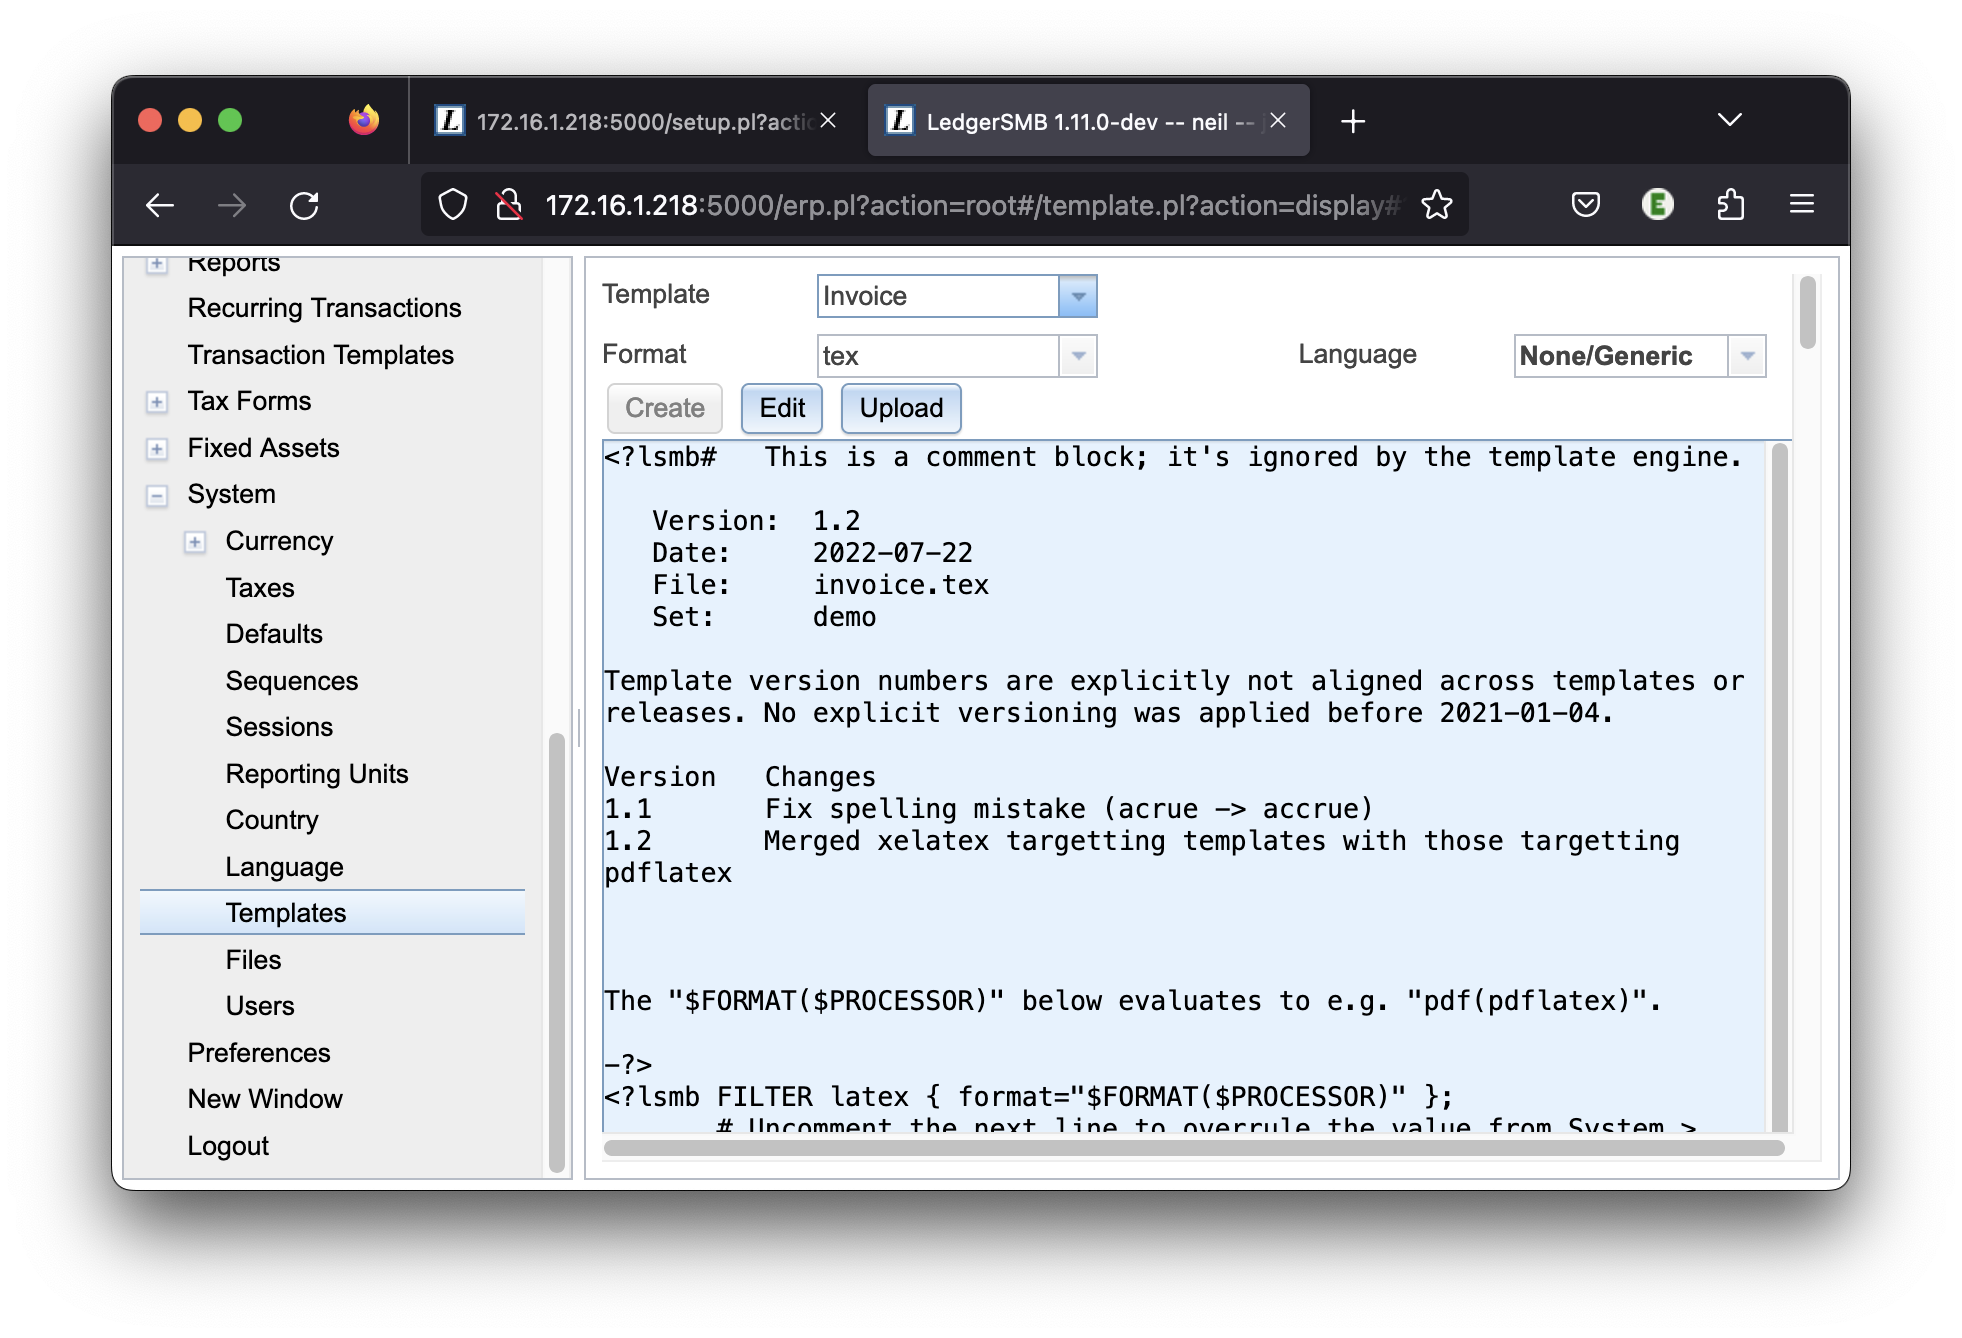
\includegraphics[width=\linewidth]{system-templates-edit-invoice.png}
        \caption{Templates edit invoice screen}
        \label{fig:system-templates-edit-invoice}
\end{figure}

To add a file to the latex template, first upload the image file to the database.  
This can be accomplished by navigating to \menupath{System \ma Files}.

To include this graphic file in your \LaTeX{} document, it needs to be retrieved from
the database and temporarily stored in a location accessible to the PDF
generator. Once the file is in the database, then the function \texttt{dbfile\_path} handles that.

For example, If the graphic file is named "FL\_Logo\_icon\_250x250.png", then add something like the following to the \LaTeX{} template using the \texttt{Edit} button.

\begin{verbatim}
\parbox[b]{.1\textwidth}{%
    \includegraphics[scale=0.7]{%
        <?lsmb dbfile_path("FL_Logo_icon_250x250.png")?>}
}
\end{verbatim}

After editing the template must be uploaded to the database using the \texttt{Upload} button.

\subsubsection{HTML templates}
\label{subsec-company-config-html-templates}

@@@TODO Add HTML specific template info.

\subsubsection{CSV templates}
\label{subsec-company-config-csv-templates}

@@@TODO Add CSV specific template information here.




\part{Administration}
\label{part:Administration}

%\section{Introduction}
%This section of the book describes which tasks and processes might need to be carried out
%on a regular basis in order to keep the application in good health and in line with
%end-users requirements.  As a result this part is more related to the functional rather
%than technical parts of the application.
%
%The fact that the tasks described in this part of the book may be recurring during the
%lifetime of the application does not exclude them from being part of the setup phase
%of LedgerSMB.  In other words: you're likely to have to dig into this section when
%creating a company as well as when maintaining it.

\chapter{Overview}
\label{cha:AdministrationOverview}

\section{Introduction}

This part of the book describes the tasks and processes that may need to be carried out
on a regular basis in order to keep the application in good health and in line with
requirements from end users.

Maintenance may require different types of system access for different types of tasks:

\begin{enumerate}
\item Within application tasks, such as user management, require an appropriately authorized
   normal application login
\item Database administration tasks, such as backups and application upgrades,
 require
   a database level login to be used with 'setup.pl'
\item Other system-level maintenance tasks, such as updating PostgreSQL or Apache, which
   require user accounts on the server hosting LedgerSMB
\end{enumerate}

% @@@ (Within-application tasks)

% @@@ (DBA tasks from setup.pl)

% @@@ (Outside-application tasks)

\chapter{User management}
\label{cha:user-management}

\section{User creation}
\label{sec:user-creation}

Users experienced with LedgerSMB 1.2 or before or SQL-Ledger (any version) are
referred to appendix \ref{sec:DifferencesUsers} to read about the differences
with version 1.3.

In order to create users, the current user must be sufficiently authorized. The user
created at application set up time is such a user.

Go to the System $\rightarrow$ Admin Users $\rightarrow$ Add User. You'll be presented the page as shown in figure \figref{fig:create-user-step1}.

\begin{figure}[h]
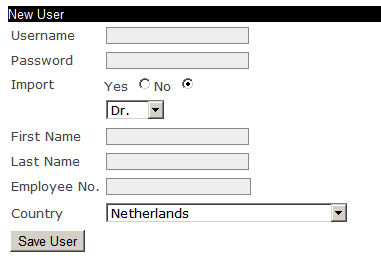
\includegraphics{create-user-step1.png}
\caption{Screen for user creation - step 1}
\end{figure}
\label{fig:create-user-step1}

The value entered in the 'Username' field will cause a database user by that name
to be created. Database users are a global resource, meaning that a collision will
occur if multiple people try to define the same user in multiple companies.
\secref{sec:UserImports} describes how to use the same user across multiple companies.

Enter the password to be used for this user into the ``Password'' field. If you're
importing a user, please leave the field empty -- that will prevent the password
from being changed.  Note that initial passwords (and password resets) are only 
valid for one day unless the user logs in and changes his/her password.

The ``Import'' field is discussed in \secref{sec:UserImports}. To create a new
user, leave the setting at ``No''.

All of the ``First Name'', ``Last Name'' and ``Employee No.'' fields are required.
However, when no employee number is specified, the system will generate one using
the sequence specified in the Defaults screen as documented in
\secref{sec:DefaultsItemNumbering}.

The ``Country'' field speaks for itself and is required as well.


\section{User authorization}


After filling out all the fields as described in the previous section and
clicking ``Save user'', you'll be presented
a second screen in the user creation process: the user authorization screen.
See \figref{fig:create-user-step2} for a screenshot of the top of that screen.

\begin{figure}[h]
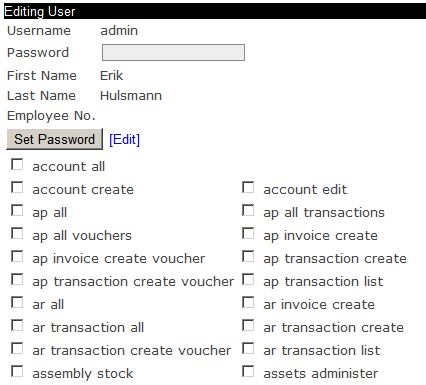
\includegraphics{create-user-step2.png}
\caption{Screen for user creation - step 2}
\label{fig:create-user-step2}
\end{figure}


The process of assigning user authorizations is the process by which the granted
access to specific parts of the application. One can imagine that - in a moderately
sized company - sales should not be editing accounting data and accountants should
not be editing sales data. Yet, in order to cooperate, both parties need to be
given access to the same application. This is where authorizations come in.

In aforementioned screen, which equals the ``Edit user'' screen, you have to assign the
newly created user his application rights. By default, the user doesn't have any
rights. Checking all check marks makes the user an application ``super user'', i.e.
gives the user all available application rights.

For a description of the roles a user can be assigned and their effects, the
reader is referred to \appref{cha:RolesListing}.


\section{Maintaining users}

\subsection{Editing user information and authorizations}

When the role of a user in the company changes, it may be necessary to assign
that user new roles and possibly revoke some other roles. This can be done through
user search: System $\rightarrow$ Admin Users $\rightarrow$ Search Users $\rightarrow$ Search $\rightarrow$ {[}edit] which brings you to the same screen as presented in
\figref{fig:create-user-step2}.

Similarly, there may be reasons to change the user information, such as a last name
(e.g. upon marriage).

Note that if you reset a password, the new password is valid for one day unless
changed.  The preferred workflow is for the individual with permissions to reset
the password, give the new password to the user, they then log in and
immediately change it.

\subsection{Changing user preferences}

Each user can change his preferences and password through the \texttt{Preferences}
top level menu. See \figref{fig:user-preferences}.

\begin{figure}[h]
\centering
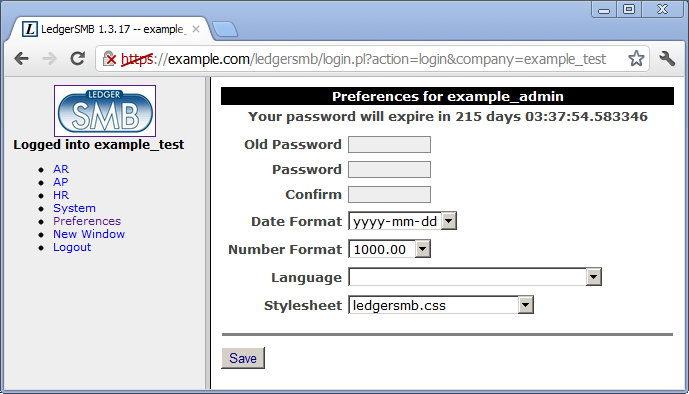
\includegraphics[width=7cm]{user-preferences.png}
\caption{User preferences screen}
\label{fig:user-preferences}
\end{figure}


\subsection{Deleting users}

From the ``User search'' result screen, users can be ``deleted'' from the company:
they have their access to the current company revoked.

@@@ Does the delete button delete the user from the cluster as well as from the application? % It looks like the API supports this but currently it is not told
             % to do so --Chris T


\section{User imports}
\label{sec:UserImports}

If a database user already exists, e.g. because this user was created to be used
with another LedgerSMB company, it can't be created a second time. In order to be
able to use that user with the current company, it needs to be ``imported'' instead.

The difference between creating a new user and importing one is that the ``Import''
radio button should be set to ``Yes'' and that you should not fill out a password.
If you do, the password of that user will be overwritten for all companies.

All other fields are still applicable: the data entered for other companies isn't
copied to the current company.


\section{setup.pl users}

Users created through the process documented above don't have enough rights to
execute actions through the setup.pl database administration tool. Note that this
is on purpose. You will need access to the server to create such users, or request
one from your application service provider (ASP) if you use a hosted solution.

During the set up process such a user is normally being created. This user can later
be used to manage the database from the database administration tool setup.pl.


\chapter{Definition of goods and services}
\label{cha:ProductsDefinition}


\section{Definition of goods}
Structure of products in the system.

\subsection{Definition of parts}
\label{sec:DefinitionOfParts}

The part entry screen consists of four parts:

\begin{enumerate}
\item Part information
\item Vendor information
\item Customer information
\item File attachments
\end{enumerate}


The paragraphs below discuss each of the four sections. The part definition section
contains both required and optional fields. The information in the remaining
three sections is entirely optional.

\subsubsection{Part information}

Every part requires the following fields to be entered:

\begin{itemize}
\item [Number] The (alphanumeric) code the company uses to identify the item
\item [Description] The (native language) description of the item, used as the default
	description on sales invoices
\item [Inventory account] The asset account used to maintain the monetary equivalent
	of the inventory amount
\item [Income account] The P\&L (income) account to post the sales revenues on
\item [COGS account] The P\&L (expense) Cost of Goods Sold (COGS) account to use
	to post cost of sold items on
\item [Sell price] The default selling price used on sales invoices
\end{itemize}

Right below the accounts selection section, there is the Tax section, which lists
all tax accounts with a check mark. Each account corresponds with a certain tax type
and rate. E.g. in the Netherlands, there's one VAT tax type (BTW) which has two rates,
one of which applies to every product. This setup requires two accounts. There's more
on the subject of sales taxes in \charef{cha:Taxes}.

The other fields in this section of the screen are optional:

\begin{itemize}
\item [List price] Informational; can be used for any (monetary) purpose
\item [Last cost] Last buying price, updated when a vendor invoice listing the current part
    is posted
\item [Markup percentage] Markup on Last cost to calculate the Sell price
\item [Image]
\item [Drawing]
\item [Microfiche]
\item [Unit] A five-character field shown on the invoice
\item [Weight] Informational; can be used by add-ons or customizations
\item [ROP] Reorder point - when the inventory drops below this number,
     the part will show up in ``Short parts'' reports
\item [Bin] The storage location in the warehouse
\end{itemize}


Apart from these fields, there are also the Make and Model paired fields. Every part
can have as many Make/Model lines as required. They are informational, but can be used
in customizations of the software.

The Average Cost and On Hand fields are output-only calculated fields. Average Cost is
calculated from the historic buying prices. On Hand is the current inventory, which is
updated when posting a vendor invoice (increased) or sales invoice (decreased).


\subsubsection{Vendor information}

This section of the screen lists one or more vendors from which the part can be
purchased, with purchasing information for the given vendor:

\begin{itemize}
\item [Vendor code] Code used by the vendor to identify the good
\item [Lead time] Lead time of the part from the vendor in days
\item [Last cost] Last price at which the good was purchased from the vendor
\item [Currency] The currency belonging to the Last cost field
\end{itemize}

\subsubsection{Customer information}

The customer information section specifies sell prices per customer or price group
where those are required to deviate from the default sell price. This mechanism exists
to support the marketing principle of categorizing customers.

\begin{itemize}
\item [Sell price]
\item [From] (inclusive)
\item [To] (inclusive)
\end{itemize}

\subsubsection{File attachments}

The process of attaching files to parts is very similar to that of
attaching files to quotations, which is covered in \secref{sec:FileAttachments}.

\subsection{Definition of part groups}

All goods and services can be categorized in 'part groups'. Upon lookup, these can
help to limit the number of matches when searching for a partial part number.

As long as no part groups have been defined, the part group assignment field doesn't
show up on the goods entry screens.

There's no requirement that a good be assigned to any specific part group if part
groups have been configured, however, a good can be assigned to more than one part group.

\subsection{Definition of assemblies}



\subsection{Definition of overhead or labour}


\subsection{The use of parts versus assemblies for multi-item-package sales}
\label{subsec:parts-vs-assemblies-for-package-sales}

Often times, one may want to sell pre-packaged multiples of a single item, such as Jack
in \charef{cha:building-up-stock} who wants to sell memory modules in pairs as well as
single items, with the price for the pair set separately from the single-item price.

There are basically two use-cases

\begin{enumerate}
\item Pre-packaged sales which are separately stocked
\item Single item sales which are achieved by unwrapping the multi-item packages
\end{enumerate}

The former case would be that of a supermarket selling packages of coffee in
singles and shrink-wrapped in pairs. These items get stocked, sold and produced separately.
Handling these is straight forward: as they are basically separate products from the point
of administration and inventory management, they're handled as separate parts.

The latter case would be Jack's case where single-item sales is achieved by unwrapping
a multi-item package. Basically, there's a single inventory for both types of packaging.
This situation can be handled (a) by creating separate parts or (b) by creating a part and an
assembly.
To reiterate: The fact that one wants to be able to separately set a pricing strategy
for the bundled items is the driver to go look for other solutions than just sell a
multiple of the original item.

There is no option which matches the actual practice: one inventory for two parts. The solution
always will keeps two separate stocks for the two items, but one may work better in practice
than the other.

Option a (separate parts) keeps the inventory of both items strictly separate,
meaning there's no way to convert between the two, other than selling and buying.

Option b (a part and an assembly) mismatches reality in so far that it will require one
to stock the single items and update the assembly stock regularly while in practice the
multi-item packages are stocked and unwrapped upon single-item sales. This procedure works
to have the assembly stock go negative on sales and restock regularly (e.g. daily) to
update assembly stock back to 0 (zero). This removes inventory from the single-item stock,
allowing for a semi-automated way to convert stock from one type of inventory to another.


\section{Definition of services}

\chapter{Chart of accounts}
\label{cha:chart-of-accounts}

\section{Accounts and headers}

The system allows ordering accounts into groups by assigning accounts to headers. Headers
can themselves be assigned to other headers resulting in trees of account groups.\footnote{Although the database structure supports this type of account hierarchy
doesn't the 1.3 user take advantage of it yet: in 1.3 accounts can be assigned a header,
but headers can't be assigned to headers themselves.}



\section{Account configuration}

Headers don't have any configuration, other than their number and description. Accounts also
have a number and description, but require additional configuration for the application to work
correctly. The settings are described in the sections that follow.

\subsection{Account options}
\label{sec:AccountOptions}
\begin{itemize}
\item Contra This checkmark identifies the account as a contra account, which means
   that the account is going to hold the opposite of an account it's associated with.
   A good example of this kind would be the depreciation account associated with a fixed
   asset account where the depreciation account contains the credit amount to be added to
   the original asset (debit) value to get the current asset value.
\item Recon This checkmark identifies the account as one which needs reconciliation as
   described in \secref{sec:Reconciliation}.
\item Tax This checkmark identifies the account as a Tax (VAT) account. Tax accounts need
   to be further configured. See \charef{cha:Taxes} for further discussion of the
   subject.
   \label{item:AccountOptionsTax}
\end{itemize}

\subsection{Summary accounts}
\label{subsec:summary-accounts}

There are currently three types of summary accounts:

\begin{enumerate}
\item AR Marking an account as a summary account for AR means that all outstanding
   receivable amounts will be posted to this account. The Accounts Receivable administration
   will contain the details of which amount is owed by which customer.
\item AP Same as the AR account, except for amounts owed to vendors.
\item Inventory This account holds the monetary value equal to the items on stock.
\end{enumerate}

\subsection{Account inclusion in drop down lists}

@@@ Add summary

\subsubsection{Receivables \& payables UI}
\label{subsec:AR-AP-checkmarks}

\begin{itemize}
\item[Income (AR\_amount)] This check mark adds the account to the list of accounts
   in the transaction and invoice screens which are used to post income on.
\item[Payment (AR\_paid)] This check mark adds the account to the list of accounts
   to choose from in the Receipts (AR) and Payments (AP) screens. Additionally, it
   adds the account to the part entry screen as described in \secref{sec:DefinitionOfParts}.
\item[Tax (AR\_tax)] This check mark makes the account show up as a check mark on the
   customer (AR) or vendor (AP) entry screen. See \charef{cha:Taxes} for further discussion.
\item[Overpayment (AR\_overpayment)] Adds the account to the receipts screen as discussed
   in \secref{sec:UsingOverpayments}.
\item[Discount (AR\_discount)] Adds the account to the customer entry screen's selection
   list for accounts to post 
\end{itemize}

The payables UI works the same way as the receivables UI. The difference is
that the technical names of the configuration identifiers are prefixed by AP\_ instead
of AR\_.

\subsubsection{Tracking Items}

The items on this line relate to stocked items, i.e. those tracked for inventory: parts and
assemblies.

\begin{enumerate}
\item[Income (IC\_sale)] Adds the account to the selection list of income accounts on the
   part and assembly definition screens.
\item[COGS (IC\_cogs)] Adds the account to the selection list of COGS @@@ accounts on the
   part, assembly and overhead definition screen.
\item[Tax (IC\_taxpart)] Adds a check mark to the part and assembly definition screen
   for the applicable account. See \charef{cha:Taxes} for more details on how taxes
   work in LedgerSMB.
\end{enumerate}

@@@ Question: Labor/Overhead accounts == inventory accounts??
  % Labor/Overhead has an inventory and expense account but no income account.
  % Chris T

\subsubsection{Non-tracking items}

The items on this line relate to untracked (non stocked) items, i.e. services.

\begin{enumerate}
\item[Income (IC\_income)] Adds the account to the income account selection list in
   the service definition screen.
\item[Expense (IC\_expense)] Adds the account to the expense account selection list in
   the service definition screen.
\item[Tax (IC\_taxservice)] Adds a check mark to the service definition screen for the
   applicable account. See \charef{cha:Taxes} for more details on how taxes work in LedgerSMB.
\end{enumerate}

\subsubsection{Fixed assets}

\begin{enumerate}
\item[Fixed asset (Fixed\_Asset)] Marks the account as holding the original asset value for the fixed
   assets module, for some classes of fixed assets.
\item[Depreciation (Asset\_Dep)] Marks the account as holding the cumulative depreciation amount
   for the fixed assets module, for some classes of fixed assets.
\item[Expense (asset\_expense)] Adds the expense account to the selection list of the fixed assets
   accounting module. See \secref{sec:FixedAssetAccounting} for more details.
\item[Gain (asset\_gain)] Account to hold book value gain upon disposal of a fixed asset.
\item[Loss (asset\_loss)] Account to hold book value loss upon disposal of a fixed asset.
\end{enumerate}


\section{Alternative accounts (GIFI)}

Next to the regular account numbering scheme, LedgerSMB supports a second numbering scheme: GIFI numbering. The GIFI accounts are a kind of secondary numbering scheme to support legal requirements.

Some jurisdictions require a specific numbering scheme, which can be supported using GIFI. If you
use GIFI account numbers, each account is associated with a GIFI account. Multiple accounts may map
to a single GIFI account.

Many General Ledger reports exist in two variants: a variant using the normal G/L accounts and
one with the GIFI numbering scheme. In the GIFI variant, when a single GIFI has multiple accounts,
the total reported under GIFI is the sum of the mapped accounts.


\subsection{Maintaining GIFI}

GIFI accounts should be created before being assigned to a standard G/L account. GIFI accounts
can be maintained through the System $\rightarrow$ Chart of accounts $\rightarrow$ Add GIFI and List GIFI menu items. Existing accounts can be edited by selecting them from the List GIFI menu, which opens a page where individual GIFI items can have their number or
description adjusted.


\chapter{Taxes}
\label{cha:Taxes}

\section{Overview}

When an account has been marked as a Tax account (see \secref{sec:AccountOptions}, item
\ref{item:AccountOptionsTax}) several things happen:

\begin{itemize}
\item The account will be shown in the customer and vendor account screens with
   a check mark to mark it ``relevant for the customer''
\item The account will be shown in the part and service configuration screens
   with a check mark to mark it ``relevant for the part/service item''
\item The account will be shown in the tax configuration screen in order to set
   a tax percentage on the account
\end{itemize}

By marking an account relevant for a customer, taxes will be calculated when
creating a sales invoice for the given customer which includes parts which also
have the specific account marked as relevant.

\section{Tax account configuration}

@@@ What does the ``order'' field do again??
% The order field is used only in cases where taxes are componding, for example
% where a province, such as Quebec is taxing the taxes collected by another tax
% authority, such as the national authority.  Taxes of a lower order are
% taxed by taxes on a higher order.
% For example:  order 0, rate 10%, and order 1, rate 5% would make:
% The first rate 10% of the total, and the second rate 5% of 110% of the total.
% -- Chris T

\section{Tax calculation plug-ins}
\label{sec:TaxRulePlugins}

The tax calculation system has been designed to handle the most complex tax system
thinkable. Because the tax calculation rules for most set ups aren't really all that
complex, LedgerSMB comes with a single tax calculation plug in out of the box: the
``Simple'' tax calculation rule.

For more complex needs, more complex routines can be developed and plugged into
LedgerSMB side-by-side with the simple rule.

\chapter{Pricing}

\section{Introduction}

In the application there are four reasons for an invoice to include a discount:

\begin{enumerate}
\item Because a discount is entered by the sales person creating the quotation,
  sales order or sales invoice
\item Because the customer's payment terms include a discount for paying early
\item Because the customer belongs to a type of business which is entitled to discounts
\label{item:PricingBusinessType}
\item Because the customer has been assigned a price matrix leading to discounts
\label{item:PricingPriceMatrix}
\end{enumerate}

This section deals with items \ref{item:PricingBusinessType} and \ref{item:PricingPriceMatrix} only.

@@@ types of business are 'old school'; price groups have been introduced to replace types of business with a more fine-grained structure.

\section{Definition of types of business}

Types of business are really straight forward: they feature a description
which allows them to be identified in the customer account screen and a discount
percentage which is applied across the board. I.e. all invoices to the customer
will have that discount applied.

\section{Definition of price groups / price matrix}

\chapter{Contingency planning}

\section{Backup and restore}

\subsection{Backup using setup.pl}

\subsection{Backup using PostgreSQL administration tools}

\subsection{Restore}

\section{Advanced PostgreSQL: replication}

\chapter{Software updates}

\section{LedgerSMB patch release roll out}

\chapter{Optional Features}

As business requirements change sometimes it may be necessary to add or remove
some of the optional features of LedgerSMB.  This chapter describes how these
optional features work, how to troubleshoot them of things go wrong, and how to
enable or disable them.

\section{PDF and Postscript Documents}

LedgerSMB can create PDF and Postscript documents for orders, invoices, and
more.  This is an optional feature and requires some additional software not
included with LedgerSMB, including a \LaTeX\ distribution and extensions to 
Perl's TemplateToolkit framework.

The PDF and PS invoices are generated using a program called \LaTeX\
which handles the layout and typesetting.  The actual \LaTeX\ files are
creating using Template Toolkit with extensions for \LaTeX.  These
extensions are in the Template::Latex package available from CPAN.
The software then generates a \LaTeX\ file which is then processed to
create a PDF or PS.

Typically the first thing to do is to install a \LaTeX\ distribution
like TexLive (distributed with many Linux distributions and available
for OSX and Windows).  This provides \LaTeX\ and many of the modules
needed.   In general I recommend that if your distro has a
texlive-extras package that you install this too.

After this is installed, you must then install Template::Latex.  This
can be done by typing on the command line:

\# cpan Template::Latex

This will also install a number of dependencies including
LaTeX::Driver, which will need to know where your LaTeX binaries are.
It is usually pretty good at finding them.

If things go wrong and you can't get it to work, the following
commands may provide useful diagnostic information when requesting
help:

From the LedgerSMB application directory:
\$ perl -MLedgerSMB::Template::Latex -e print

From the doc/manual directory in the LedgerSMB application directory:
\# pdflatex LedgerSMB-manual

\section{Attaching Uploaded Files to PDF Invoices}

\section{OpenDocument Spreadsheet Output}

\section{Microsoft Excel Output}





\part{Workflows}
\label{part:Workflows}

\chapter{Customers and vendors}

\section{Creating customers and vendors}

\section{Multiple customers within one company}

\section{Creating vendors from customers}

\section{}

\section{Maintaining contact information}


\chapter{Quotations from Vendors and for Customers}

\section{Creating Quotations and RFQs}

\chapter{Sales and vendor orders}

\section{Creating new orders}

\section{Creating orders from quotations}

\section{Creating orders from projects}

\section{Creating purchase orders from sales orders}

\section{Combining orders}

\section{Recurring orders}


\chapter{Sales and vendor invoices}

\section{Creating new invoices}

-- this section is about Sales and Vendor Invoices

\section{Creating invoices from orders}



\section{Invalidating invoices}

Sometimes, it's necessary to invalidate an invoice. When an invoice has been
posted, this also means derived administrations have been updated, such as
inventory for the items on the invoice.

To undo the effects of an invoice, i.e. to reduce the amount outstanding with a
customer, use the \texttt{VOID} button on the invoice screen as shown in @@@figref .
This creates a new invoice by the same number as the original, except that the new
invoice has a suffix \texttt{-VOID}.

\begin{quotation}
Unfortunately, in LedgerSMB 1.3 - the earlier versions - voiding an invoice did not
automatically close the original and voiding invoices.  To close both invoices from
the open invoice overview, use the cash receipt process as described in
\secref{sec:SinglePayments} to make a zero amount payment.
\end{quotation}

\section{Correcting and deleting invoices}
\label{sec:CorrectingInvoices}

There's only one way to persist an invoice in LedgerSMB: posting it. This means
the invoice becomes part of the accounting information. One of the primary
properties of an accounting system is to record full audit trails and help enforce
internal controls as detailed in \secref{sec:AccountingSystemRequirements}. Because
of that fact there's no way to delete or edit invoices after they have been posted
\footnote{LedgerSMB currently does not support saving an invoice without posting
it. This functionality is on the roadmap for addition when the AR/AP functionality
is being rewritten - currently 1.5 or 1.6.}.

The only way to ``undo'' an invoice is by voiding it. This is important for several
reasons:

\begin{enumerate}
\item Invoices can't be deleted (because they're accounting data)
\item Invoices pose a claim on the assets of a customer
\label{item:InvoicesAsClaims}
\item @@@ others?
\end{enumerate}

Specifically item \ref{item:InvoicesAsClaims} is important: when you sent the invoice
to your customer, you effectively sent them a claim. When you decide to refrain from
pursuing that claim, you should notify them of that fact so they have the documentation
to update their accounting system to reflect that fact: they need your documentation
to void their vendor invoice, instead of paying it.

For the same reason it's ill-advised (and no longer supported) to edit invoices:
when a customer has multiple invoices, each stating a different amount, all
using the same invoice number; how is that customer supposed to document (verifiably)
that the claim has been settled satisfactorily by paying the one he did?

\subsection{Credit and debit notes}



\subsection{Credit and debit invoices}



\chapter{Shop sales}

\section{Opening and closing the cash register}

\section{Shop sales invoices}


\chapter{Manufacturing management}

\section{Producing sales orders}

\subsection{Work orders}


\chapter{Inventory management}

\section{Shipping}

\subsection{Pick lists}
\subsection{Packing list}

\section{Receiving}

\section{Partial shipments}

\section{Transferring between warehouses}

\section{Inventory reporting}



\chapter{Accounts receivable and payable}

\section{Creating generic AR/AP items}

\section{Handling refunds, overpayments and advances}

- this bit is about credit notes and debit notes

\section{Handling returns}

--> this bit is about credit (sales) and debit (vendor) invoices

\chapter{Credit risk management}

\section{Introduction}

A company runs credit risk when it gives credit: it runs the risk of the
creditor not paying off its debts.  LedgerSMB features two ways to manage
the risks involved:

\begin{enumerate}
\item Limit management
\item Arrears management
\end{enumerate}

The former tries to limit the risk involved by making sure no customer
receives more credit than a certain limit while the latter tries to
make sure any over due payments get cashed.

\section{Limit management}

Limit management should prevent a company on one hand from delivering too much
to its customers at once and on the other from taking (and delivering) new orders
to customers with too high amount of unpaid invoices.

@@@ Where to set up limits

@@@ How to monitor limits


\section{Managing arrears}

As mentioned before, the process of managing arrears is directed toward
detecting arrears positions with customers early and taking appropriate
action.


\subsection{Monitoring AR aging}

In order to find out about over due invoices, a company should run the AR
aging report available under AR $\rightarrow$ Reports $\rightarrow$ AR Aging.
The initial screen presents parameters for the aging report to be generated.

@@@ discuss parameters

This report shows customers and their outstanding invoices categorised as:

\begin{description}
\item [Current] Invoices not over due
\item [30] Invoice amounts over due by 30 days or less
\item [60] Invoice amounts over due by 60 days or less (but more than 30)
\item [90] Invoice amounts over due by 90 days or less (but more than 60)
\end{description}


@@@ Printing / mailing aging reports to customers


\subsection{Tracking invoice history}

After an invoice becomes over due a process will be started to remind
the customer of the outstanding amount requiring payment.

In order to keep records of actions taken to chase customer payment,
the invoice screen has an ``Internal Notes'' field which can be edited
after the invoice has been posted.

In order to save any edits to that field, hit the ``Save Info'' button.

\begin{quotation}
Note that the ``Save Info'' button also saves any changes to the ``TaxForm'' column or
rather, any information that's not accounting information (posted to the books and
thereby fixed) nor information which appears on the invoice - which also should remain
unedited in order to be able to generate an exact copy at a later date.
\end{quotation}


\subsection{Special treatment of invoices}

There may be good reasons to treat some over due invoices differently. E.g. in case
payment arrangements have been made with the customer and further standard arrears
management would not be appropriate any more.

In this case, you can put an invoice ``On Hold''. The opposite of being on hold is
being active. The AR Aging report allows selection of all invoices, only active
invoices (those not on hold) or only invoices on hold.


\section{Interest on arrears}

\section{Allowance for doubtful accounts}

\section{Writing off bad debt}

\subsection{Direct write-off}

\subsection{Allowed-for write-off}


\chapter{Receipts and payment processing}


\section{Single receipts and payments}
\label{sec:SinglePayments}

\section{Batch receipts and payments}


\section{Check payments}


\section{Using overpayments}
\label{sec:UsingOverpayments}

\section{Receipt and payment reversal}

\section{Receipts and payments in foreign currencies}

\chapter{Accounting}

\section{Separation of duties: Transaction approval}
\label{sec:SeparationOfDuties}

\section{Period closing}

\section{Bank reconciliation}
\label{sec:Reconciliation}

\section{Year-end processing}

\section{Tax (VAT) reporting}

\begin{itemize}
\item 1099
\item EU VAT
\end{itemize}

\section{Entering general accounting documents}

\section{Fixed asset accounting}
\label{sec:FixedAssetAccounting}

\section{Reporting}
\subsection{Income statement}
\subsection{Balance sheet}
\subsection{Trial balance}



% !TeX encoding = UTF-8
% !TeX spellcheck = en_US
% !TeX root = ledgersmb-book.tex

\part{General Operation}
\label{part-general-operation}

\chapter{User Interface}
\label{cha-general-operation-user-interfacei}
Description of the general operation of LedgerSMB that appears across multiple views in the application and that are not described elsewhere.

\section{Reports}
\label{sec-general-operation-user-interface-reports}

At the bottom of most report views there is a '[permalink]'. The idea of a \gls{permalink}\index{permalink} is that you get a link which you can share with your colleagues and when inserted into the browser, returns exactly the same report (or at least a search with exactly the same parameters as you used).  To copy a  \gls{permalink} the user can right-click and select "Copy link" from the drop down menu and pass it to a colleague by pasting into an email or other messaging App.

\part{Customization}
\label{part-customization}

\chapter{Overview}
\label{cha-customization-overview}

\section{Introduction}
\label{sec-customization-overview-introduction}

Customization\index{customization} is about adding or changing behavior of an application in ways that were not foreseen when it was written.  This differs from configuration\index{configuration}, because the latter can be used to select between planned behaviors.  Since the functionality or behavior to be added wasn't foreseen, this means that customization implies application code being added or changed.  Especially changing existing behavior has proven problematic (in the IT industry at large) in terms of being able to later upgrade the underlying software to newer releases.  This problem can be mitigated by creation of specific ``extension points''\index{extension points}: places in the software which are designed to expand or replace existing behaviors.

LedgerSMB has several such ``extension points'':

\begin{itemize}
	\item Workflow configuration
	\item Dependency-injection based configuration:
		\begin{itemize}
			\item Document formatters
			\item Bank statement importers
			\item HTTP request handlers/interceptors
			\item Outgoing mail transport
		\end{itemize}
	\item Sales/VAT tax calculation
\end{itemize}

Each bank has its own format for bank statement\index{bank statements} exports, making it impossible to develop import functionality that's generically usable.  Some default importers come with LedgerSMB - mostly as example code for those developing their own.  The dependency injection-based configuration supports adding these user-specific developments without changing any of the files that come in the standard distribution.

Another example is changing ``Workflow configuration''\index{workflow configuration}, by which the life cycle of invoices and GL transactions can be changed.  This way, additional steps can be introduced into the life cycle, or steps can be combined (from a user perspective) by automatically executing steps after another has been triggered manually.

Customization usually means additional or modified Perl code needs to be loaded. 

@@@TODO: describe where to store this new or overriding code...

\section{Workflow configuration}
\label{sec-customization-workflow-configuration}

LedgerSMB uses the concept of workflows\index{workflows} to manage object life cycle.
An invoice, for example, may be \texttt{saved}, \texttt{posted} or \texttt{reversed}.  These
are states in the life cycle of the invoice.  Each state may have associated actions. E.g. in
case of the invoice there may be a \texttt{Post} action when it's \texttt{saved} or to
\texttt{E-mail} it when it's \texttt{posted}.  Actions may cause the document to change state:
if the \texttt{Post} action is executed on a \texttt{saved} invoice, its new state
will be \texttt{posted}.  E-mailing an invoice does not change its state: it
remains posted.  Instead, a new workflow is created which manages state of the e-mail.

 \IfFileExists{./wf1.pdf}{
 	\begin{figure}[H]
		\centering
		% 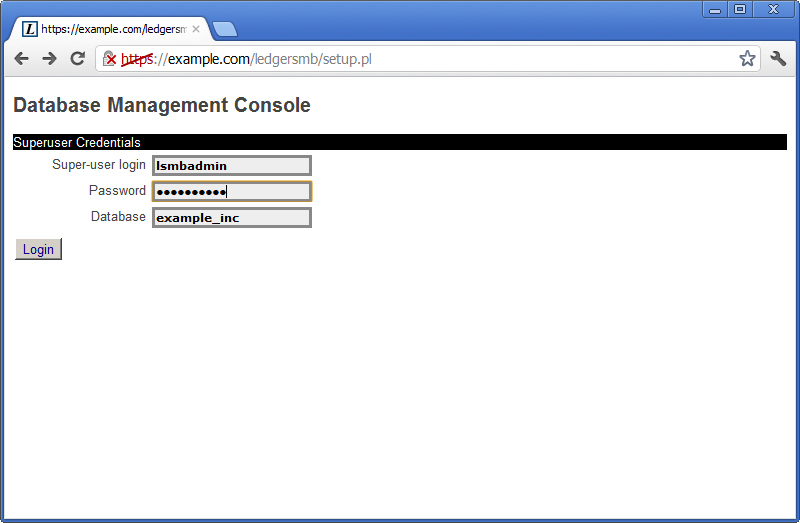
\includegraphics[width=0.8\textwidth]{dmc-create-step1.png}
		% HTML processing does not handle cropping of this image, need to figure out why?
		% 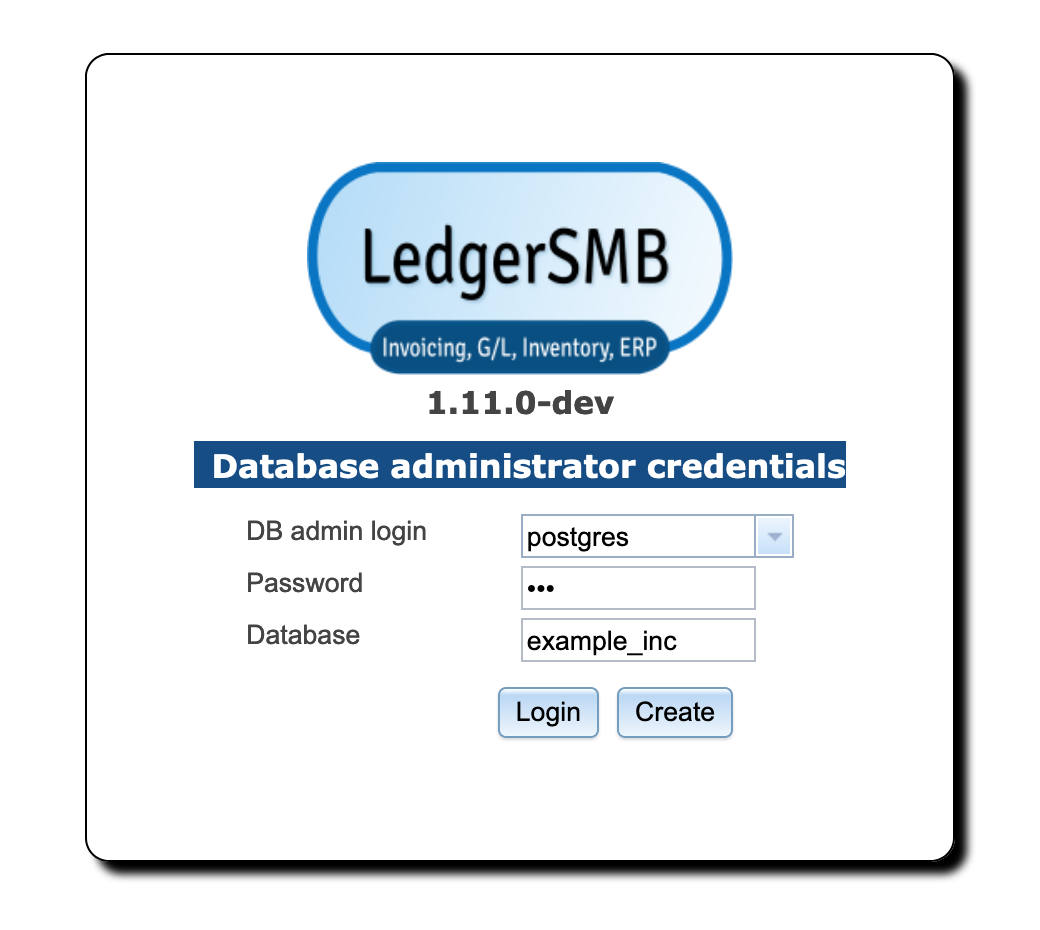
\includegraphics[width=\graphicswidth,  trim={0pt 50 0 0}, clip]{\autoscreenshotdir/setup-pl-login.png}
		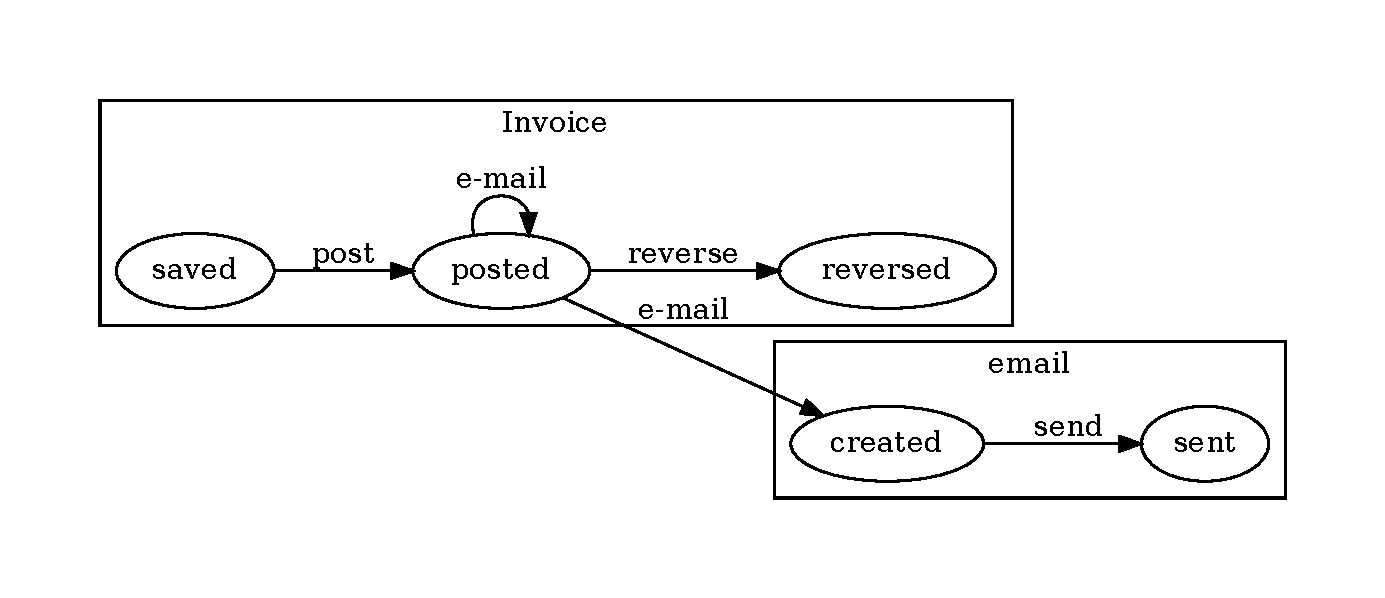
\includegraphics[width=\graphicswidth]{wf1.pdf}
		\caption{Workflow triggered from another workflow}
		\label{fig:triggered-workflow}
	\end{figure}
}{
	\begin{figure}
	\digraph[scale=0.4]{wf1}{
		rankdir=LR;
		subgraph invoice {
			graph [label="Invoice"];
			cluster = true;
			saved -> posted [label="post"];
			posted -> reversed [label="reverse"];
		};
	
	    subgraph email {
	    	graph [label="email"];
	    	cluster = true;
	    	created -> sent [label="send"];
	    };
	
	    posted -> created [label="e-mail"];
	    posted -> posted [label="e-mail"];
	
	}
	\caption{Workflow triggered from another workflow}
	\label{fig:triggered-workflow}
	\end{figure}
}

Actions belonging to a state may (or may not) be available. This is determined by one or
more conditions.  Examples are ``is the posting date of the transaction in a closed period''
and ``is the current user allowed to post transactions''.  When the condition evaluates to
\texttt{false}, the action is not available.

Workflows are configurable. Configurations list the following aspects:

\begin{enumerate}
	\item A list of states
	\item A list of allowable actions per state
	\item A list of conditions per action
	\item A mapping of actions to Perl code
	\item A mapping of conditions to Perl code
\end{enumerate}

With these ingredients, the software's behavior can be changed.  E.g. by adding a new state
and action in the invoice, an extra reviewing pairs of eyes can be added to the posting process.
By adding a condition on this action, it can be made required for invoices over 100.000 USD
(but not for other invoices).

\IfFileExists{./wf2.pdf}{
	\begin{figure}[H]
		\centering
		% 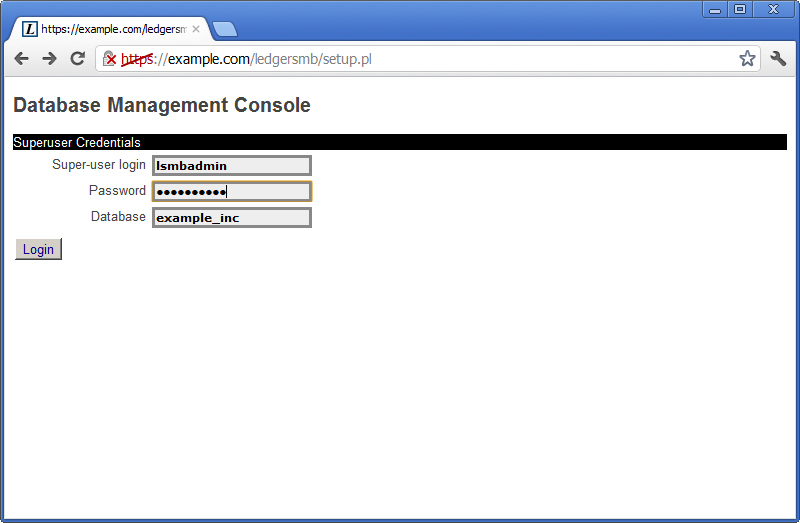
\includegraphics[width=0.8\textwidth]{dmc-create-step1.png}
		% HTML processing does not handle cropping of this image, need to figure out why?
		% 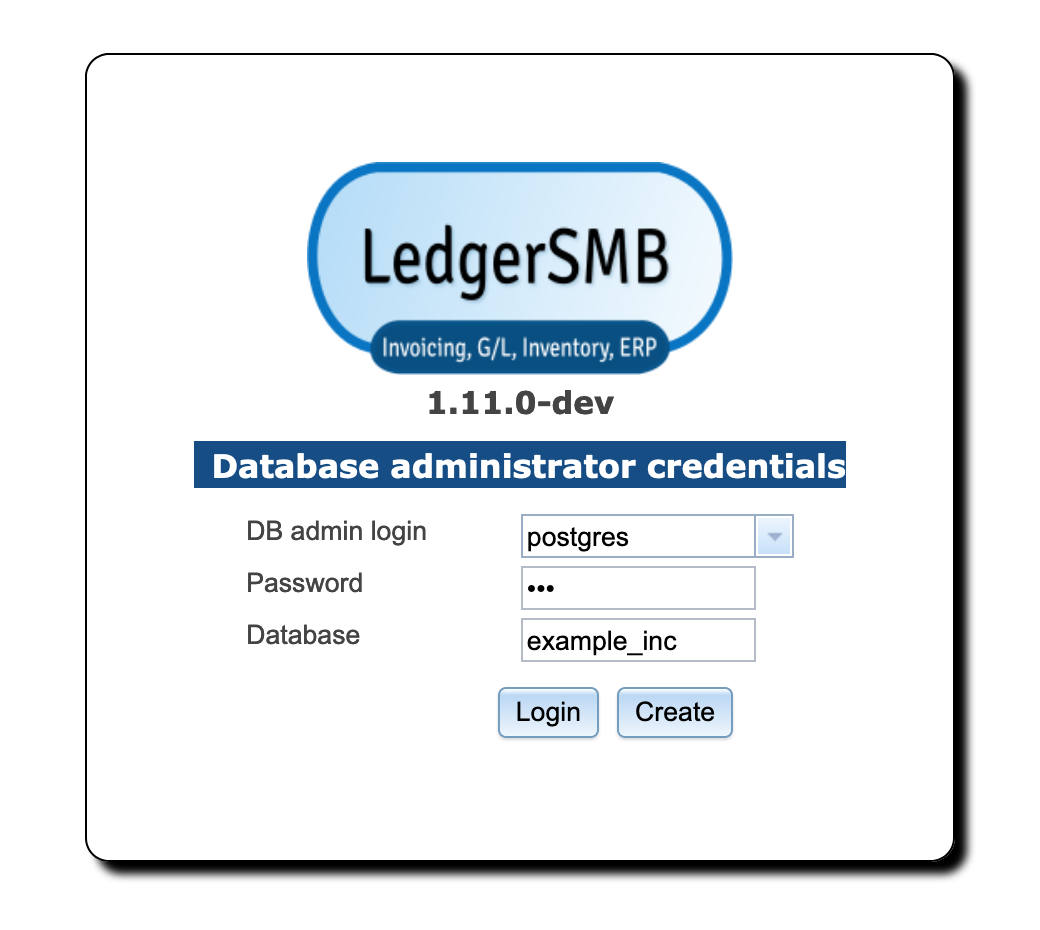
\includegraphics[width=\graphicswidth,  trim={0pt 50 0 0}, clip]{\autoscreenshotdir/setup-pl-login.png}
		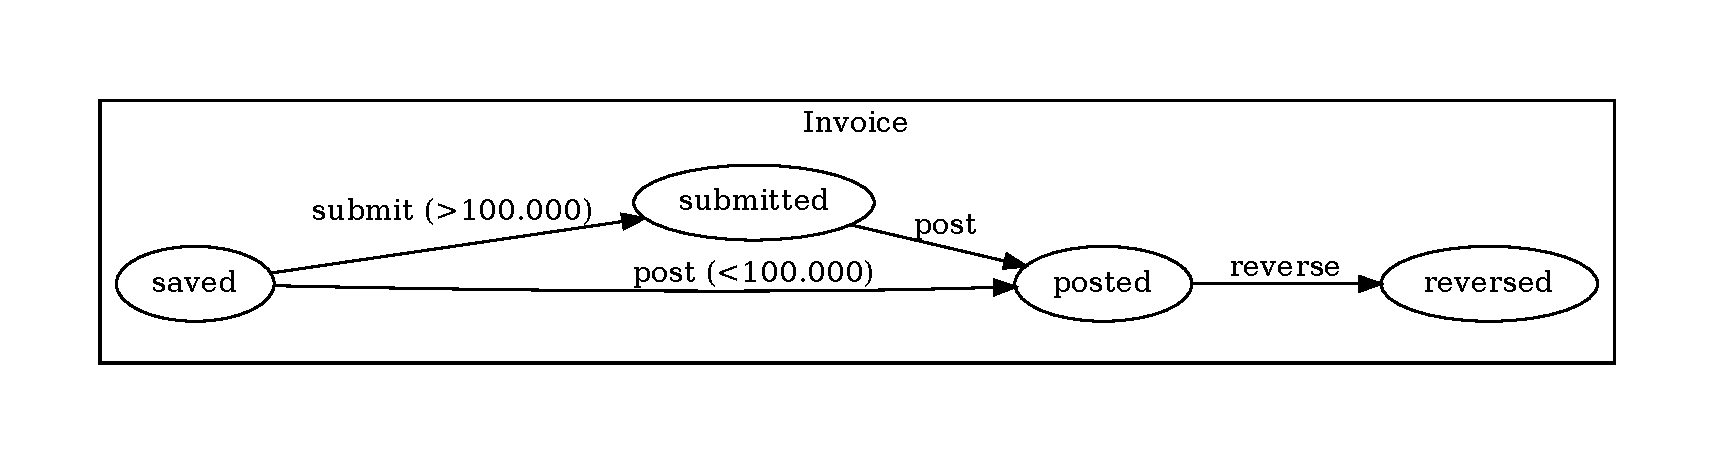
\includegraphics[width=\graphicswidth]{wf2.pdf}
		\caption{Conditional workflow actions}
		\label{fig:conditional-workflows}
	\end{figure}
}{
	\begin{figure}
		\digraph[scale=0.4]{wf2}{
			rankdir=LR;
			subgraph invoice {
				graph [label="Invoice"];
				cluster=true;
				saved -> posted [label="post (<100.000)"];
				saved -> submitted [label="submit (>100.000)"];
				submitted -> posted [label="post"];
				posted -> reversed [label="reverse"]
			}
		}
		\caption{Conditional workflow actions}
		\label{fig:conditional-workflows}
	\end{figure}
}

By changing association of the \texttt{save} action with its code, the application will act
differently when saving the invoice.  Customizations may associate new behaviors with existing
actions or create new ones entirely.  The behavior does not need to be known by the application
developers, as the association may point to code added to the local installation.  This way, a
\texttt{remind} action can be added to posted invoices, triggering a text (SMS) message to the
customer.


Workflows are stored in the \texttt{./workflows/} directory.  Each workflow consists of
several files, prefixed with the name of the workflow (e.g. \texttt{ar-ap.} for 'AR/AP' workflows):

\begin{description}
	\item [\texttt{ar-ap.actions.xml}] (optional) names the list of available transitions
	in the workflow naming Perl code to be executed
	\item [\texttt{ar-ap.conditions.xml}] (optional) names the list of conditions to be used
	in the workflow naming Perl code to evaluate
	\item [\texttt{ar-ap.persisters.xml}] (optional) defines the Perl mechanism to load and store
	workflow instances
	\item [\texttt{ar-ap.workflow.xml}] (required) defines the life cycle by combining states with
	the actions and conditions listed in the respective configuration files. Each state lists
	the allowable actions with the conditions to enable the action and a resulting state.
\end{description}

Customized versions of workflow definition files must be stored in \linebreak
 \texttt{./customized\_workflows/}\footnote{See
 	\secref{subsec-global-config-ledgersmb-yaml} on how to configure
 these paths}.  Files stored in this directory will be used to override those in
the standard location: the file\linebreak \texttt{./custom\_workflows/ar-ap.workflow.xml} will replace the built-in workflow
from \texttt{./workflows/ar-ap.workflow.xml} used for invoices and \linebreak AR/AP transactions.
No changes should be made directly to the standard files because of the risk that those
files will be overwritten on upgrade -- loosing the changes.

Next to the per-workflow files, there is a generic definition file for actions,
conditions and persisters.  Elements defined in these files can be used in all
workflows; those elements defined in the per-workflow files can only be used
in the specific workflow.

The engine driving workflow state management is the
Workflow\footnote{\url{https://metacpan.org/pod/Workflow}} library.  See its
documentation on MetaCPAN as well as the built-in workflows as examples of how
to define one's own.

\subsection{Workflow observers}
\label{subsec-customization-workflow-observers}

Particularly interesting is the concept of observers\index{workflow observers}:
this functionality allows the application to be extended based a specific action
occurring without changing the life cycle.  An example could be to create a PayPal
payment request when an invoice is posted: an observer could be ``listening'' to
``AR/AP'' workflow events which at some point will flag the state of the invoice
becoming \texttt{posted}.

\subsubsection{Notes on Quote, Order, AR, AP and GL workflow customization}
\label{subsubsec-customization-workflow-observers-notes}

The actions in the workflows \texttt{order-quote}, \texttt{ar-ap} and \texttt{gl} are
hard coded\footnote{This is not a permanent situation, but rather a consequence of
these workflows being used in \gls{oldcode}\index{old code}}.  This means that the list of actions is restricted to those defined in the
files \texttt{order-quote.actions.xml}, \texttt{ar-ap.actions.xml} and
\texttt{gl.actions.xml}.  It's not necessary to use all actions in the workflow, but
additional ones cannot be created -- contrary to what is in the \texttt{Workflow}
documentation.

The \texttt{class} attribute for most actions in these workflows is set to the value
\texttt{LedgerSMB::Workflow::Action::Null}.  This means it does nothing.  Rather, it
doesn't do anything \textit{in addition to} what the action already does in its hard
coded implementation.  Setting the action's class attribute to some other value allows
the developer to add behavior on top of what's hard coded.

\section{Document formatters}
\label{sec-customization-document-formatters}

Document formatters transform templates into output documents; e.g. an HTML invoice
template can be transformed into an HTML file with the details of the invoice filled
out.  LedgerSMB comes with a number of built-in formatters.  Additional ones could be
implemented to transform HTML documents to PDF (replacing the traditional \LaTeX to PDF)
or the creation of eInvoices\index{eInvoice} in the format of the local jurisdiction.

The generation of output entails these steps (preceded by the process to find a
suitable document formatter):

\begin{itemize}
	\item Loading the input template from the database
	\item Preprocessing the input variables using the formatter's \texttt{encode}
		function
	\item Initializing the template expansion using the formatter's \texttt{setup} function
	\item Expanding the template using \texttt{Template::Toolkit}
	\item Post-processing the expanded output using the formatter's \texttt{postprocess}
\end{itemize}

A custom formatter needs to implement the protocol as documented at \url{https://docs.ledgersmb.org/perl-api/1.11.0/LedgerSMB/Template.pm.html#FORMATS}.

\section{Bank statement importers}
\label{sec-customization-bank-importers}

LedgerSMB comes with three bank statement importers built-in:

\begin{itemize}
	\item [CAMT.053] The \gls{ISO20022}\index{ISO20022} ``Cash Management'' message 053
		(Bank-to-Customer account statement)
	\item [\gls{OFX}\index{OFX}] A standard to exchange data describing financial transactions
	\item [CSV]  File based using \gls{csv}\index{csv}
\end{itemize}

The bank statement importer is a Perl class implementing the
\texttt{LedgerSMB::Reconciliation::Format} role; it parses a file with bank
transactions, extracting the fields expected by the bank reconciliation procedure:

\begin{itemize}
	\item [amount] The amount involved in the transaction; negative if the bank
		reports a credit amount, positive when it's a debit
	\item [date] The date on which the amount contributed to the bank account balance
	\item [source] An identifier by which the bank identifies the transaction; to be
		used for matching with the ``Source'' field in the bank ledger
	\item [type] Information clarifying the transaction; e.g. Cash, ACH, etc.
\end{itemize}

The CSV parser has many options to accommodate the tremendous variance that can be
observed in CSV files.  When using a custom bank reconciliation procedure \textit{or}
when the bank makes a more exotic format available, customization of the bank statement
importer may be necessary.

\section{HTTP request interceptors}
\label{sec-customization-http-requests}

@@@TODO: describe how to add \texttt{Plack::Middleware} instances in the request processing

\section{Outgoing mail transport}
\label{sec-customization-outgoing-mail}

The library used for sending e-mail (\texttt{Email::Sender})
includes a wide variety of transports that can be used to configure the library to (pretend to) send
e-mail messages.  For a list of available transports, see \url{https://metacpan.org/dist/Email-Sender}.

Should a different delivery method be required even considering the list of available transports,
this can be achieved by implementing a custom \texttt{Email::Sender::Transport}.

\section{Sales/VAT tax calculation}
\label{sec-customization-sales-tax}

Tax calculations performed for VAT and/or sales taxes have been abstracted into so-called
``tax modules''.  An example of a custom tax module can be found in the directory
\texttt{utils/wa-tax-service} in the source repository.

Before tax modules can be used, they need to be registered in the \texttt{taxmodule} table.

\textbf{Important:} Please note that there is a tight integration between the database "pointing"
to the tax module and the web server which expects to be able to \textit{load} this Perl code to
perform the prescribed calculations.
If for some reason the application looses the ability to load the Perl module, this will break
the ability to create or view invoices.

\chapter{Batch data import methods}
\label{cha-customization-batch-import}

\section{Custom bank statement import}
\label{sec-customization-batch-import-bank-statement}

\section{Chart of Accounts import}
\label{subsec-customization-import-coa}

This function allows bulk import of an entire chart of accounts using a
single \gls{csv} file.

The first line of the file contains the headers of the columns. The
import routine expects the columns as presented in (table name).

\begin{description}
\item [accno] Number of the account or header
\item [desc] Description for the account or header
\item [charttype] ``H'' for heading record \\
``A'' for account record
\item [category] ``I'' for Income \\
``E'' for Expense \\
``A'' for Asset \\
``L'' for Liability
\item [contra] ``0'' not a \gls{contra}\index{contra} account \\
``1'' is a \gls{contra} account
\item [tax] ``0'' not a tax account \\
``1'' is a tax account.
\item [link] A colon (':') separated list of account check-mark values (links) as described
    in \secref{subsec-coa-account-links}, or ``AR'', ``AP'' or ``IC'' for the specified summary accounts
\item [heading] ``accno'' of the heading to group the account (or heading) under
\item [gifi] \gls{gifi} account number
\end{description}

All lines after the first one are considered to be data lines.

\chapter{Add-ons and plug-ins}
\label{cha-customization-add-ons}

\chapter{Company creation}
\label{cha-customization-company-creation}

\section{Template sets}\index{templates}
\label{sec-customization-company-creation-templates}




\part{Appendices}
\appendix

\chapter{Differences between version 1.2 and 1.3}

\section{Users}
\label{sec:DifferencesUsers}

The way users are defined and used differs greatly between LedgerSMB 1.3 and
older versions. In version 1.3 user access to the database is enforced by the
database itself. This means that users logging in to the LedgerSMB web application
are in reality logging into the PostgreSQL database. In older versions, the web
app would verify the user's credentials (using a common database connection used
for all users).

The difference between these approaches is that security is no longer (solely)
maintained by the web application - with all inherent risks. Instead, the database
now plays an important role as well. The effect is that the LedgerSMB team now
leverages the experience of the PostgreSQL community - a highly respected community
well known for its security focus - to make sure your data stays secure.

This structure also enables LedgerSMB 1.3 to offer separation of duties and
authorizations throughout the application without being required to do a full
rewrite of the application.

It's this shift in paradigm that makes it impossible to meaningfully migrate
users from older LedgerSMB and SQL-Ledger versions to LedgerSMB 1.3.


\chapter{Migration}

\section{Introduction}

There are plenty of reasons to want to migrate to LedgerSMB 1.3:

\begin{enumerate}
\item Separation of duties
\item Security better integrated into the application
\item Better, more strict data model
\label{item:StricterDataModel}
\item Some important sources of user error eliminated
\item Better workflows for cash reconciliation
\item @@@ others?
\end{enumerate}

Yet, while item \ref{item:StricterDataModel} is a good reason to want to switch, it's
also a reason why migration from older versions to 1.3 can be harder than earlier
migrations: when the data
in your older version is not consistent, it won't fit into the new data model and
will need to be fixed first.

Especially if your database has a very long line of history, being migrated trough
lots of SQL-Ledger and LedgerSMB versions, you may want to consider asking for help
from a professional party. It could save you a lot of time.

However, don't be discouraged and have a go yourself first. Just be sure to run
your upgrade on a backup database: the migration process is non-destructive, but
in case accounting data is involved: better safe than sorry!

Also it is worth noting that a number of automatic checks are performed on your
data prior to migration, and to the extent possible, you are given an
opportunity to fix those issues identified.  Because these checks are
pre-migration checks, they are written to your old data and will persist after
backing out of a migration to 1.3.

\section{From older LedgerSMB versions}

\section{From SQL-Ledger 2.8}

\section{From older SQL-Ledger versions}

\section{From other accounting packages}

While accounting and ERP solution have wildly differing structures to record their
data, this sections uses data with a relatively simple structure as a show case of
how this problem may be dealt with.

\begin{quote}
Note that the encoding you use to transfer to the database depends on the settings
used to create the PostgreSQL database with.  A migration is a good moment to think
about encodings an solve older encoding issues.  Now would be a good moment to
anticipate the requirement for accented characters and non-western alphabets: set up
a UTF-8 encoded database and recode your data accordingly.
\end{quote}

\subsection{Migrating customers}

The source system for this section uses a structure where every company has one
contact person, one address, one phone number and e-mail.

In order to understand how to migrate this data structure to LedgerSMB, it's
important to understand that:

\begin{enumerate}
\item The company from the source maps to the \emph{Company} and \emph{Entity} entities
\item The contact person maps to the \emph{Entity Credit Account} entity
\item The address maps to the \emph{Location} entity - and requires a location class: Sales, Billing or Shipping
\item The phone number, fax number and e-mail map to \emph{Contact items}
\end{enumerate}

The reason behind the separation between the \emph{Company} and \emph{Entity} entities
is that every customer is an \emph{Entity}, but not all entities are companies, since
some entities are \emph{Person}s - natural persons.

@@@ How to

\subsection{Migrating parts, services, ...}
\subsection{Migrating open items}
\subsection{Migrating your ledger}

\chapter{Listing of application roles}
\label{cha:RolesListing}

Application roles specify the right to execute one or more tasks in the application.
LedgerSMB enforces these roles by allowing a user to select (list, read) data from or to
insert (create), update (edit) or delete (delete) data in the tables holding the data
related to the execution of these tasks.

\begin{description}
\item [account\_all] Allows the user to both create new and edit existing GL accounts.
\item [account\_create] Allows the user to create (but not edit) new GL accounts.
\item [account\_edit] Allows the user to edit (but not create) GL accounts.
\item [ap\_all]
\item [ap\_all\_transactions]
\item [ap\_all\_vouchers]
\item [ap\_invoice\_create]
\item [ap\_invoice\_create\_voucher]
\item [ap\_transaction\_create]
\item [ap\_transaction\_create\_voucher]
\item [ap\_transaction\_list]
\item [ar\_all]
\item [ar\_invoice\_create] Allows the user to create and update sales invoices. If the
   user needs to be able to enter invoices in foreign currencies, the
   \emph{exchangerate\_edit} role must be assigned as well.
\item [ar\_transaction\_all] @@@ I miss the symmetry with AP here??
% just added it -- Chris T
\item [ar\_transaction\_create]
\item [ar\_transaction\_create\_voucher]
\item [ar\_transaction\_list]
\item [assembly\_stock]
\item [assets\_administer]
\item [assets\_approve]
\item [assets\_depreciate]
\item [assets\_enter]
\item [auditor]
\item [audit\_trail\_maintenance]
\item [backup] \emph{Superseeded}. This role has been replaced by backup functionality
   in setup.pl
\item [batch\_create] Allows the user to create new batches.
\item [batch\_list]
\item [batch\_post] Allows the user to post batches; this authorization includes the
   right to search for batches (and therefore includes \emph{batch\_list})
\item [business\_type\_all]
\item [business\_type\_create]
\item [business\_type\_edit]
\item [cash\_all]
\item [close\_till]
\item [contact\_all\_rights]
\item [contact\_create]
\item [contact\_edit]
\item [contact\_read]
\item [department\_all]
\item [department\_create]
\item [department\_edit]
\item [draft\_edit]
\item [employees\_manage]
\item [file\_attach\_order]
\item [file\_attach\_part]
\item [file\_attach\_tx]
\item [file\_read]
\item [financial\_reports]
\item [gifi\_create]
\item [gifi\_edit]
\item [gl\_all]
\item [gl\_reports]
\item [gl\_transaction\_create]
\item [gl\_voucher\_create]
\item [inventory\_all]
\item [inventory\_receive]
\item [inventory\_reports]
\item [inventory\_ship]
\item [inventory\_transfer]
\item [language\_create]
\item [language\_edit]
\item [list\_all\_open]
\item [manual\_translation\_all]
\item [orders\_generate]
\item [orders\_manage]
\item [orders\_purchase\_consolidate]
\item [orders\_sales\_consolidate]
\item [orders\_sales\_to\_purchase]
\item [part\_create]
\item [part\_edit]
\item [partsgroup\_translation\_create]
\item [part\_translation\_create]
\item [payment\_process]
\item [pos\_all]
\item [pos\_cashier]
\item [pos\_enter]
\item [pricegroup\_create]
\item [pricegroup\_edit]
\item [print\_jobs]
\item [print\_jobs\_list]
\item [project\_create]
\item [project\_edit]
\item [project\_order\_generate]
\item [project\_timecard\_add]
\item [project\_timecard\_list]
\item [project\_translation\_create]
\item [purchase\_order\_create]
\item [purchase\_order\_edit]
\item [purchase\_order\_list]
\item [receipt\_process]
\item [reconciliation\_all]
\item [reconciliation\_approve]
\item [reconciliation\_enter]
\item [recurring]
\item [rfq\_create]
\item [rfq\_list]
\item [sales\_order\_create]
\item [sales\_order\_edit]
\item [sales\_order\_list]
\item [sales\_quotation\_create]
\item [sales\_quotation\_list]
\item [sic\_all]
\item [sic\_create]
\item [sic\_edit]
\item [system\_admin]
\item [system\_settings\_change]
\item [system\_settings\_list]
\item [taxes\_set]
\item [tax\_form\_save]
\item [template\_edit]
\item [users\_manage]
\item [voucher\_delete]
\item [warehouse\_create]
\item [warehouse\_edit]
\item [yearend\_run]
\end{description}

\chapter{Open source explained}

\section{An open source application}

\section{An open source book}


\chapter{Copyright and license}

Copyright (c) 2011, 2012 Erik H\"ulsmann.


This work is licensed under the Creative Commons Attribution License.
To view a copy of this license, visit \url{http://creativecommons.org/licenses/by/3.0/}
or send a letter to Creative Commons, 559 Nathan Abbott Way,
Stanford, California 94305, USA.

A summary of the license is given below, followed by the full legal text.

\section{License summary}

\begin{verbatim}

You are free:
  * to share -- to copy, distribute and transmit the work
  * to remix -- to adapt the work


Under the following condition:
  You must attribute he work in the manner specified by the author or licensor
  (but in a way that suggests that they endorse you or your use of the work).


With the understanding that:
  Waiver -- Any of the above conditions can be waived if you get permission
            from the copyright holder.
  
  Other rights -- In no way are any of the following rights affected by the license:
     * Your fair dealing or fair use rights, or other applicable 
         copyright exceptions and limitations;
     * The author's moral rights;
     * Rights other persons may have either in the work itself or
         in how the work is used, such as publicity or privacy rights.



\end{verbatim}



\section{Legal full text}

\begin{verbatim}
License

THE WORK (AS DEFINED BELOW) IS PROVIDED UNDER THE TERMS OF THIS 
CREATIVE COMMONS PUBLIC LICENSE ("CCPL" OR "LICENSE"). THE WORK
IS PROTECTED BY COPYRIGHT AND/OR OTHER APPLICABLE LAW. ANY USE OF
THE WORK OTHER THAN AS AUTHORIZED UNDER THIS LICENSE OR COPYRIGHT
LAW IS PROHIBITED.

BY EXERCISING ANY RIGHTS TO THE WORK PROVIDED HERE, YOU ACCEPT AND
AGREE TO BE BOUND BY THE TERMS OF THIS LICENSE. TO THE EXTENT THIS
LICENSE MAY BE CONSIDERED TO BE A CONTRACT, THE LICENSOR GRANTS
YOU THE RIGHTS CONTAINED HERE IN CONSIDERATION OF YOUR ACCEPTANCE
OF SUCH TERMS AND CONDITIONS.

1. Definitions

"Adaptation" means a work based upon the Work, or upon the Work
and other pre-existing works, such as a translation, adaptation,
derivative work, arrangement of music or other alterations of a
literary or artistic work, or phonogram or performance and
includes cinematographic adaptations or any other form in which
the Work may be recast, transformed, or adapted including in any
form recognizably derived from the original, except that a work
that constitutes a Collection will not be considered an Adaptation
for the purpose of this License.
For the avoidance of doubt, where the Work is a musical work,
performance or phonogram, the synchronization of the Work in
timed-relation with a moving image ("synching") will be considered
an Adaptation for the purpose of this License.

"Collection" means a collection of literary or artistic works, such
as encyclopedias and anthologies, or performances, phonograms or
broadcasts, or other works or subject matter other than works
listed in Section 1(f) below, which, by reason of the selection
and arrangement of their contents, constitute intellectual
creations, in which the Work is included in its entirety in
unmodified form along with one or more other contributions, each
constituting separate and independent works in themselves, which
together are assembled into a collective whole. A work that
constitutes a Collection will not be considered an Adaptation
(as defined above) for the purposes of this License.

"Distribute" means to make available to the public the original
and copies of the Work or Adaptation, as appropriate, through sale
or other transfer of ownership.

"Licensor" means the individual, individuals, entity or entities
that offer(s) the Work under the terms of this License.

"Original Author" means, in the case of a literary or artistic
work, the individual, individuals, entity or entities who created
the Work or if no individual or entity can be identified, the
publisher; and in addition (i) in the case of a performance the
actors, singers, musicians, dancers, and other persons who act,
sing, deliver, declaim, play in, interpret or otherwise perform
literary or artistic works or expressions of folklore; (ii) in the
case of a phonogram the producer being the person or legal entity
who first fixes the sounds of a performance or other sounds; and,
(iii) in the case of broadcasts, the organization that transmits
the broadcast.

"Work" means the literary and/or artistic work offered under the
terms of this License including without limitation any production
in the literary, scientific and artistic domain, whatever may be
the mode or form of its expression including digital form, such as
a book, pamphlet and other writing; a lecture, address, sermon or
other work of the same nature; a dramatic or dramatico-musical work;
a choreographic work or entertainment in dumb show; a musical
composition with or without words; a cinematographic work to
which are assimilated works expressed by a process analogous to
cinematography; a work of drawing, painting, architecture,
sculpture, engraving or lithography; a photographic work to which
are assimilated works expressed by a process analogous to
photography; a work of applied art; an illustration, map, plan,
sketch or three-dimensional work relative to geography, topography,
architecture or science; a performance; a broadcast; a phonogram;
a compilation of data to the extent it is protected as a
copyrightable work; or a work performed by a variety or circus
performer to the extent it is not otherwise considered a literary
or artistic work.

"You" means an individual or entity exercising rights under this
License who has not previously violated the terms of this License
with respect to the Work, or who has received express permission
from the Licensor to exercise rights under this License despite
a previous violation.

"Publicly Perform" means to perform public recitations of the
Work and to communicate to the public those public recitations,
by any means or process, including by wire or wireless means or
public digital performances; to make available to the public
Works in such a way that members of the public may access these
Works from a place and at a place individually chosen by them;
to perform the Work to the public by any means or process and
the communication to the public of the performances of the Work,
including by public digital performance; to broadcast and
rebroadcast the Work by any means including signs, sounds or
images.

"Reproduce" means to make copies of the Work by any means
including without limitation by sound or visual recordings and
the right of fixation and reproducing fixations of the Work,
including storage of a protected performance or phonogram in
digital form or other electronic medium.

2. Fair Dealing Rights. Nothing in this License is intended to
reduce, limit, or restrict any uses free from copyright or rights
arising from limitations or exceptions that are provided for in
connection with the copyright protection under copyright law or
other applicable laws.

3. License Grant. Subject to the terms and conditions of this License,
Licensor hereby grants You a worldwide, royalty-free, non-exclusive,
perpetual (for the duration of the applicable copyright) license to
exercise the rights in the Work as stated below:

to Reproduce the Work, to incorporate the Work into one or more
Collections, and to Reproduce the Work as incorporated in the
Collections;
to create and Reproduce Adaptations provided that any such
Adaptation, including any translation in any medium, takes
reasonable steps to clearly label, demarcate or otherwise identify
that changes were made to the original Work. For example, a
translation could be marked "The original work was translated from
English to Spanish," or a modification could indicate "The
original work has been modified.";
to Distribute and Publicly Perform the Work including as
incorporated in Collections; and,
to Distribute and Publicly Perform Adaptations.
For the avoidance of doubt:

Non-waivable Compulsory License Schemes. In those jurisdictions
in which the right to collect royalties through any statutory
or compulsory licensing scheme cannot be waived, the Licensor
reserves the exclusive right to collect such royalties for any
exercise by You of the rights granted under this License;
Waivable Compulsory License Schemes. In those jurisdictions in
which the right to collect royalties through any statutory or
compulsory licensing scheme can be waived, the Licensor waives
the exclusive right to collect such royalties for any exercise
by You of the rights granted under this License; and,
Voluntary License Schemes. The Licensor waives the right to
collect royalties, whether individually or, in the event that
the Licensor is a member of a collecting society that
administers voluntary licensing schemes, via that society, from
any exercise by You of the rights granted under this License.
The above rights may be exercised in all media and formats
whether now known or hereafter devised. The above rights include
the right to make such modifications as are technically
necessary to exercise the rights in other media and formats.
Subject to Section 8(f), all rights not expressly granted by
Licensor are hereby reserved.

4. Restrictions. The license granted in Section 3 above is
expressly made subject to and limited by the following
restrictions:

You may Distribute or Publicly Perform the Work only under
the terms of this License. You must include a copy of, or the
Uniform Resource Identifier (URI) for, this License with every
copy of the Work You Distribute or Publicly Perform. You may
not offer or impose any terms on the Work that restrict the
terms of this License or the ability of the recipient of the
Work to exercise the rights granted to that recipient under
the terms of the License. You may not sublicense the Work. You
must keep intact all notices that refer to this License and to
the disclaimer of warranties with every copy of the Work You
Distribute or Publicly Perform. When You Distribute or Publicly
Perform the Work, You may not impose any effective technological
measures on the Work that restrict the ability of a recipient
of the Work from You to exercise the rights granted to that
recipient under the terms of the License. This Section 4(a)
applies to the Work as incorporated in a Collection, but this
does not require the Collection apart from the Work itself to
be made subject to the terms of this License. If You create
a Collection, upon notice from any Licensor You must, to the
extent practicable, remove from the Collection any credit as
required by Section 4(b), as requested. If You create an
Adaptation, upon notice from any Licensor You must, to the
extent practicable, remove from the Adaptation any credit as
required by Section 4(b), as requested.
If You Distribute, or Publicly Perform the Work or any
Adaptations or Collections, You must, unless a request has
been made pursuant to Section 4(a), keep intact all copyright
notices for the Work and provide, reasonable to the medium or
means You are utilizing: (i) the name of the Original Author
(or pseudonym, if applicable) if supplied, and/or if the
Original Author and/or Licensor designate another party or
parties (e.g., a sponsor institute, publishing entity,
journal) for attribution ("Attribution Parties") in Licensor's
copyright notice, terms of service or by other reasonable
means, the name of such party or parties; (ii) the title of
the Work if supplied; (iii) to the extent reasonably
practicable, the URI, if any, that Licensor specifies to be
associated with the Work, unless such URI does not refer to the
copyright notice or licensing information for the Work;
and (iv) , consistent with Section 3(b), in the case of an
Adaptation, a credit identifying the use of the Work in the
Adaptation (e.g., "French translation of the Work by Original
Author," or "Screenplay based on original Work by Original
Author"). The credit required by this Section 4 (b) may be
implemented in any reasonable manner; provided, however, that
in the case of a Adaptation or Collection, at a minimum such
credit will appear, if a credit for all contributing authors
of the Adaptation or Collection appears, then as part of these
credits and in a manner at least as prominent as the credits
for the other contributing authors. For the avoidance of doubt,
You may only use the credit required by this Section for the
purpose of attribution in the manner set out above and, by
exercising Your rights under this License, You may not
implicitly or explicitly assert or imply any connection
with, sponsorship or endorsement by the Original Author,
Licensor and/or Attribution Parties, as appropriate, of
You or Your use of the Work, without the separate, express
prior written permission of the Original Author, Licensor
and/or Attribution Parties.
Except as otherwise agreed in writing by the Licensor or as
may be otherwise permitted by applicable law, if You Reproduce,
Distribute or Publicly Perform the Work either by itself or
as part of any Adaptations or Collections, You must not distort,
mutilate, modify or take other derogatory action in relation to
the Work which would be prejudicial to the Original Author's
honor or reputation. Licensor agrees that in those
jurisdictions (e.g. Japan), in which any exercise of the right
granted in Section 3(b) of this License (the right to make
Adaptations) would be deemed to be a distortion, mutilation,
modification or other derogatory action prejudicial to the
Original Author's honor and reputation, the Licensor will
waive or not assert, as appropriate, this Section, to the
fullest extent permitted by the applicable national law, to
enable You to reasonably exercise Your right under
Section 3(b) of this License (right to make Adaptations)
but not otherwise.

5. Representations, Warranties and Disclaimer

UNLESS OTHERWISE MUTUALLY AGREED TO BY THE PARTIES IN WRITING,
LICENSOR OFFERS THE WORK AS-IS AND MAKES NO REPRESENTATIONS
OR WARRANTIES OF ANY KIND CONCERNING THE WORK, EXPRESS,
IMPLIED, STATUTORY OR OTHERWISE, INCLUDING, WITHOUT
LIMITATION, WARRANTIES OF TITLE, MERCHANTIBILITY, FITNESS FOR
A PARTICULAR PURPOSE, NONINFRINGEMENT, OR THE ABSENCE OF
LATENT OR OTHER DEFECTS, ACCURACY, OR THE PRESENCE OF ABSENCE
OF ERRORS, WHETHER OR NOT DISCOVERABLE. SOME JURISDICTIONS DO
NOT ALLOW THE EXCLUSION OF IMPLIED WARRANTIES, SO SUCH
EXCLUSION MAY NOT APPLY TO YOU.

6. Limitation on Liability.

EXCEPT TO THE EXTENT REQUIRED BY APPLICABLE LAW, IN NO EVENT
WILL LICENSOR BE LIABLE TO YOU ON ANY LEGAL THEORY FOR ANY
SPECIAL, INCIDENTAL, CONSEQUENTIAL, PUNITIVE OR EXEMPLARY
DAMAGES ARISING OUT OF THIS LICENSE OR THE USE OF THE WORK,
EVEN IF LICENSOR HAS BEEN ADVISED OF THE POSSIBILITY OF SUCH
DAMAGES.

7. Termination

This License and the rights granted hereunder will terminate
automatically upon any breach by You of the terms of this
License. Individuals or entities who have received Adaptations
or Collections from You under this License, however, will not
have their licenses terminated provided such individuals
or entities remain in full compliance with those licenses.
Sections 1, 2, 5, 6, 7, and 8 will survive any termination
of this License. Subject to the above terms and conditions,
the license granted here is perpetual (for the duration of
the applicable copyright in the Work). Notwithstanding the
above, Licensor reserves the right to release the Work under
different license terms or to stop distributing the Work at
any time; provided, however that any such election will not
serve to withdraw this License (or any other license that has
been, or is required to be, granted under the terms of this
License), and this License will continue in full force and
effect unless terminated as stated above.

8. Miscellaneous

Each time You Distribute or Publicly Perform the Work or a
Collection, the Licensor offers to the recipient a license
to the Work on the same terms and conditions as the license
granted to You under this License. Each time You Distribute
or Publicly Perform an Adaptation, Licensor offers to the
recipient a license to the original Work on the same terms and
conditions as the license granted to You under this License.
If any provision of this License is invalid or unenforceable
under applicable law, it shall not affect the validity or
enforceability of the remainder of the terms of this License,
and without further action by the parties to this agreement,
such provision shall be reformed to the minimum extent
necessary to make such provision valid and enforceable.
No term or provision of this License shall be deemed waived
and no breach consented to unless such waiver or consent shall
be in writing and signed by the party to be charged with
such waiver or consent.
This License constitutes the entire agreement between the
parties with respect to the Work licensed here. There are
no understandings, agreements or representations with respect
to the Work not specified here. Licensor shall not be bound
by any additional provisions that may appear in any
communication from You. This License may not be modified
without the mutual written agreement of the Licensor and You.
The rights granted under, and the subject matter referenced,
in this License were drafted utilizing the terminology of the
Berne Convention for the Protection of Literary and Artistic
Works (as amended on September 28, 1979), the Rome Convention
of 1961, the WIPO Copyright Treaty of 1996, the WIPO
Performances and Phonograms Treaty of 1996 and the Universal
Copyright Convention (as revised on July 24, 1971). These
rights and subject matter take effect in the relevant
jurisdiction in which the License terms are sought to be
enforced according to the corresponding provisions of the
implementation of those treaty provisions in the applicable
national law. If the standard suite of rights granted under
applicable copyright law includes additional rights not
granted under this License, such additional rights are deemed
to be included in the License; this License is not intended
to restrict the license of any rights under applicable law.

\end{verbatim}






\end{document}

